\documentclass[cn,pad,chinese,chinesefont=nofont]{elegantbook}
\usepackage{latexgit}
%\usepackage{showframe}
\setCJKmainfont{Source Han Serif} 
\setCJKsansfont{Source Han Sans} 
\setCJKmonofont{Source Han Mono} 
\setCJKfamilyfont{zhsong}{Source Han Serif}
\setCJKfamilyfont{zhhei}{Source Han Sans} 
\setCJKfamilyfont{zhkai}{Source Han Mono} 
\setCJKfamilyfont{zhfs}{Source Han Mono} 
\newcommand*{\songti}{\CJKfamily{zhsong}} 
\newcommand*{\heiti}{\CJKfamily{zhhei}} 
\newcommand*{\kaishu}{\CJKfamily{zhkai}} 
\newcommand*{\fangsong}{\CJKfamily{zhfs}}

\title{洞箫演奏入门手册}
\author{雪散舞}
\date{\gitcommitdate}
\cover{dongxiao/cover.jpeg}
\logo{monk.png}
\extrainfo{凤箫声动,玉壶光转,一夜鱼龙舞。}
\version{\gitcommithash}

\begin{document}
\maketitle
\frontmatter
\tableofcontents
\mainmatter

\centering
\chapter{筒音做‘低音5’}
\section{指法表}
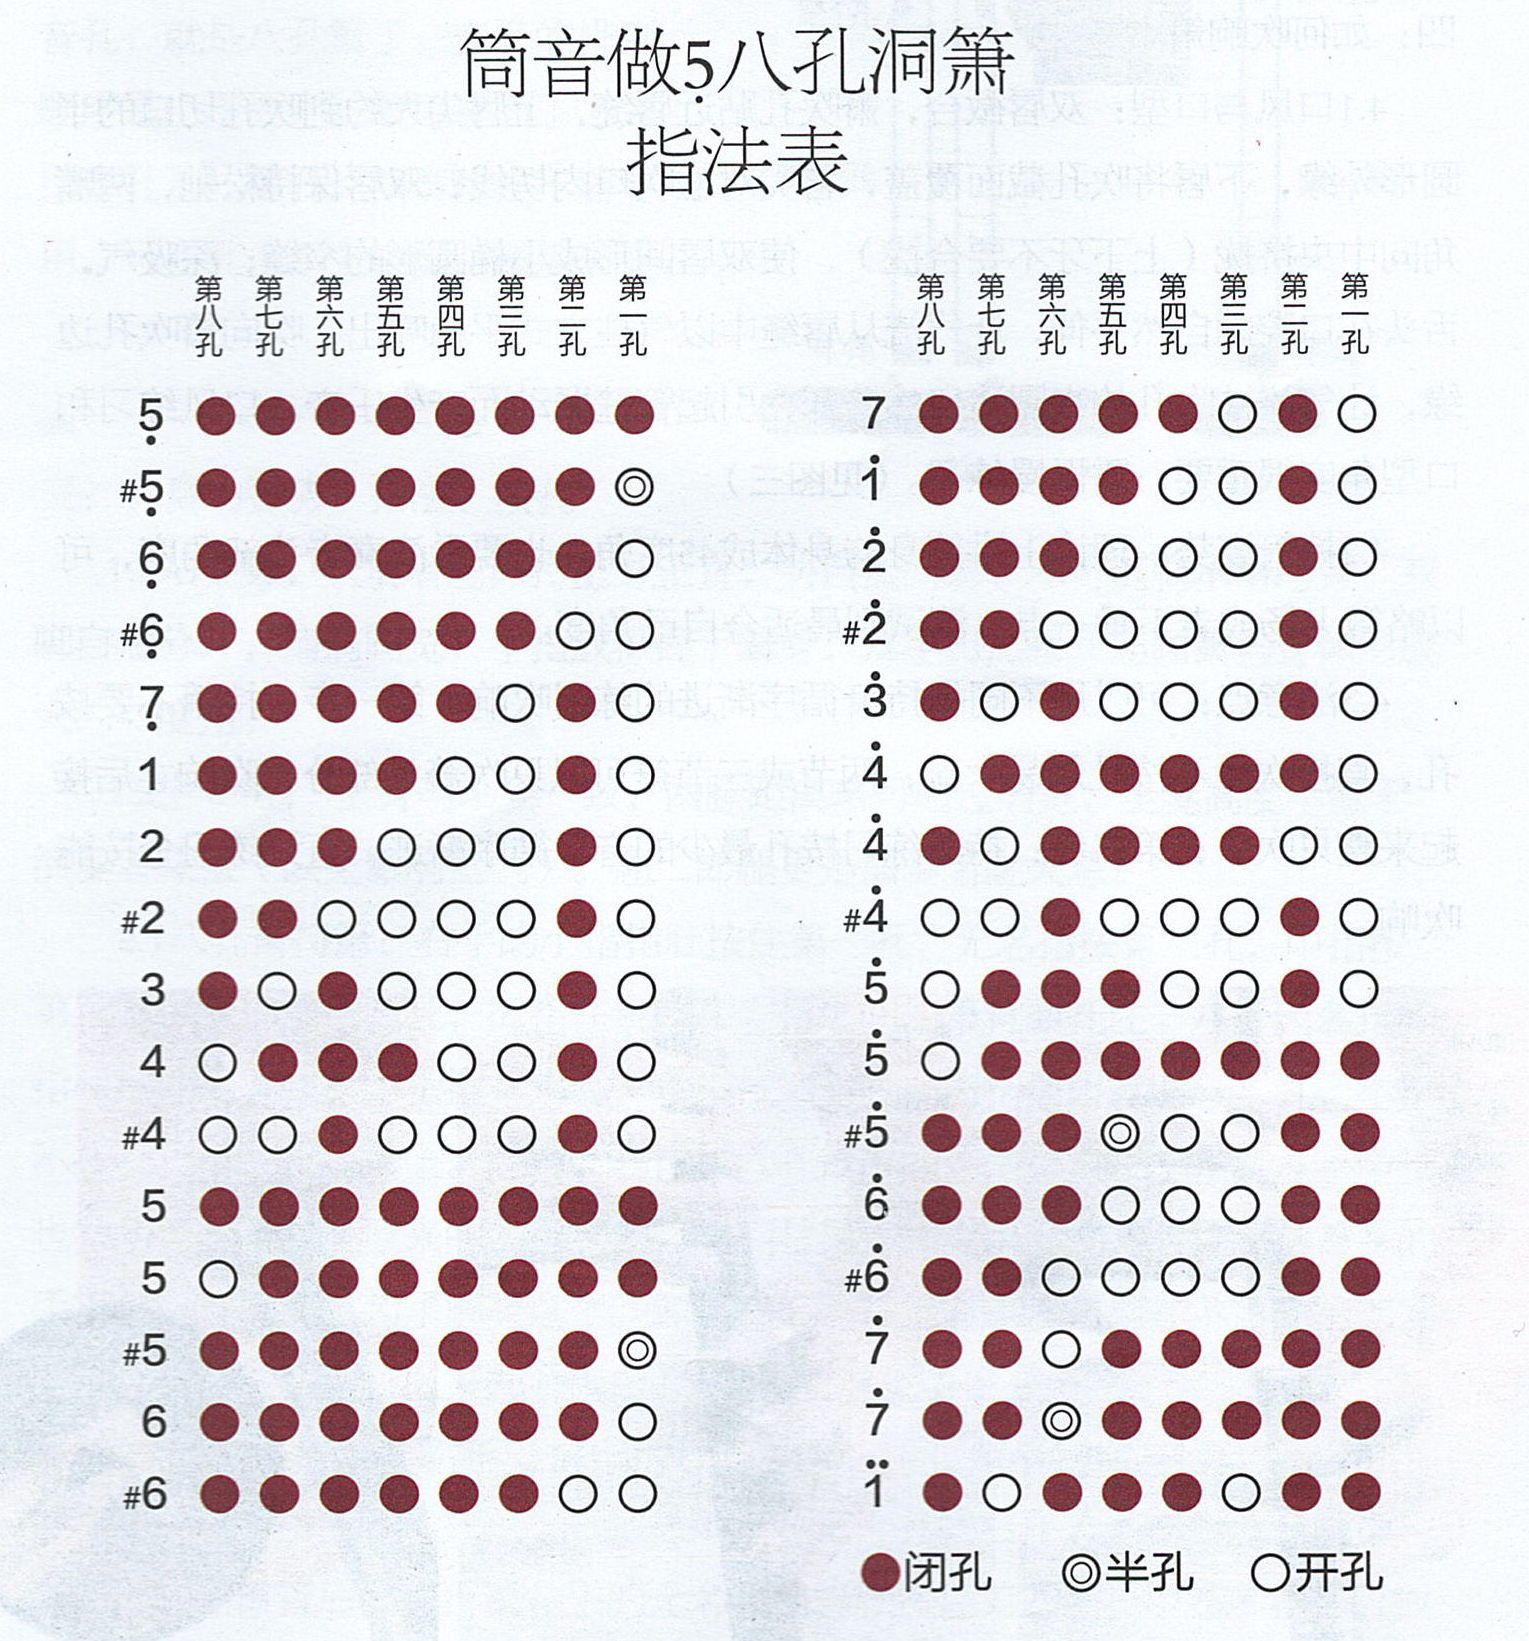
\includegraphics[width=\textwidth]{dongxiao/Scan.jpeg}

\section{练习(1)1=G}
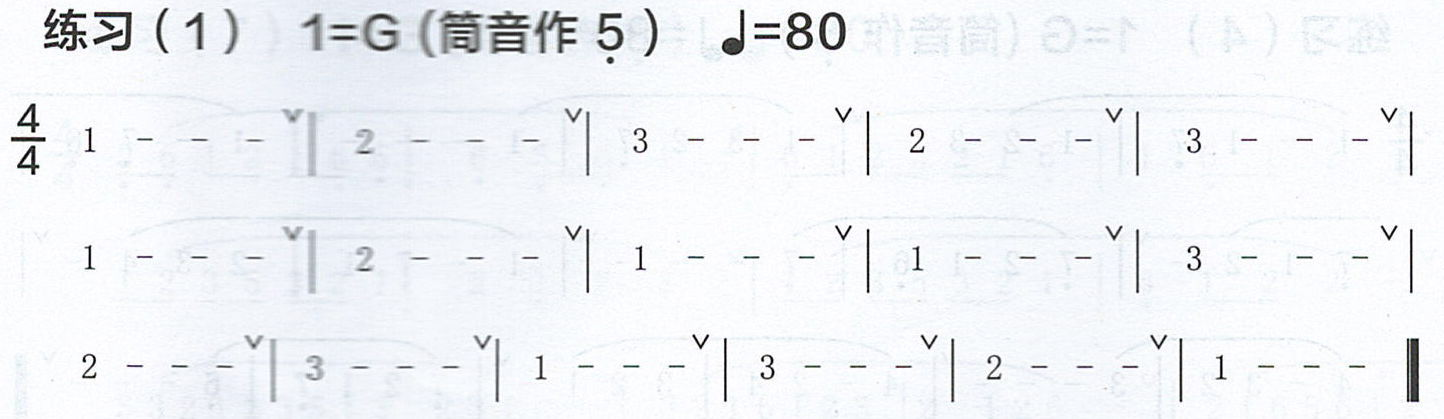
\includegraphics[width=\textwidth]{dongxiao/Scan 1-1.jpeg}
\section{练习(2)1=G}
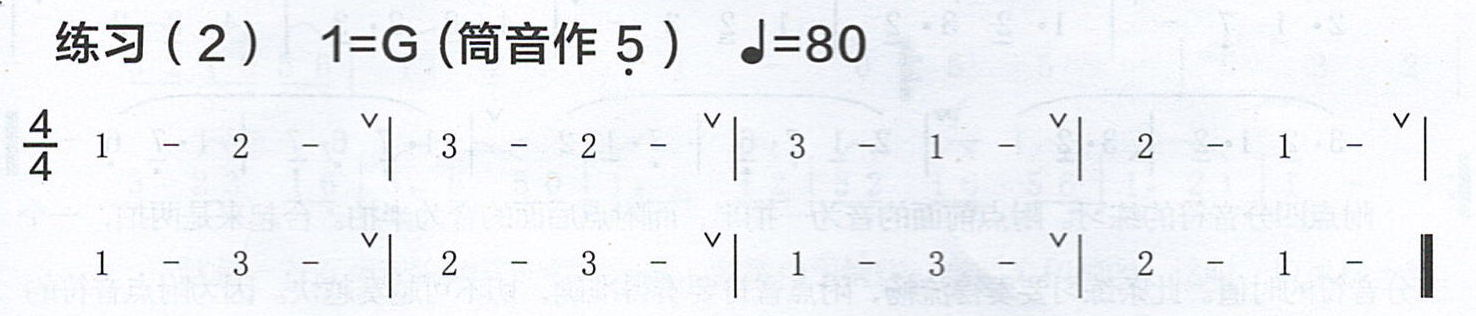
\includegraphics[width=\textwidth]{dongxiao/Scan 1-2.jpeg}
\section{练习(3)1=G}
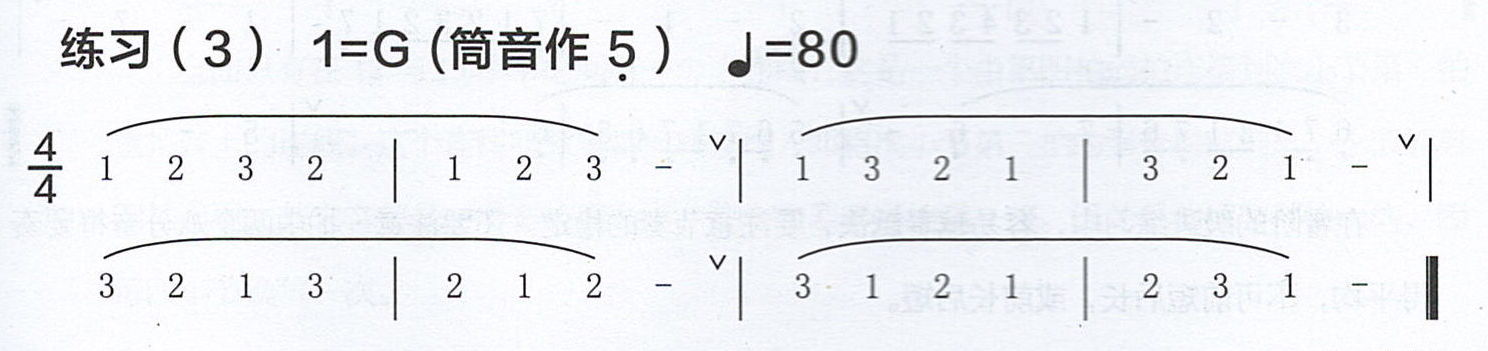
\includegraphics[width=\textwidth]{dongxiao/Scan 1-3.jpeg}

\section{练习(4-6)1=G}
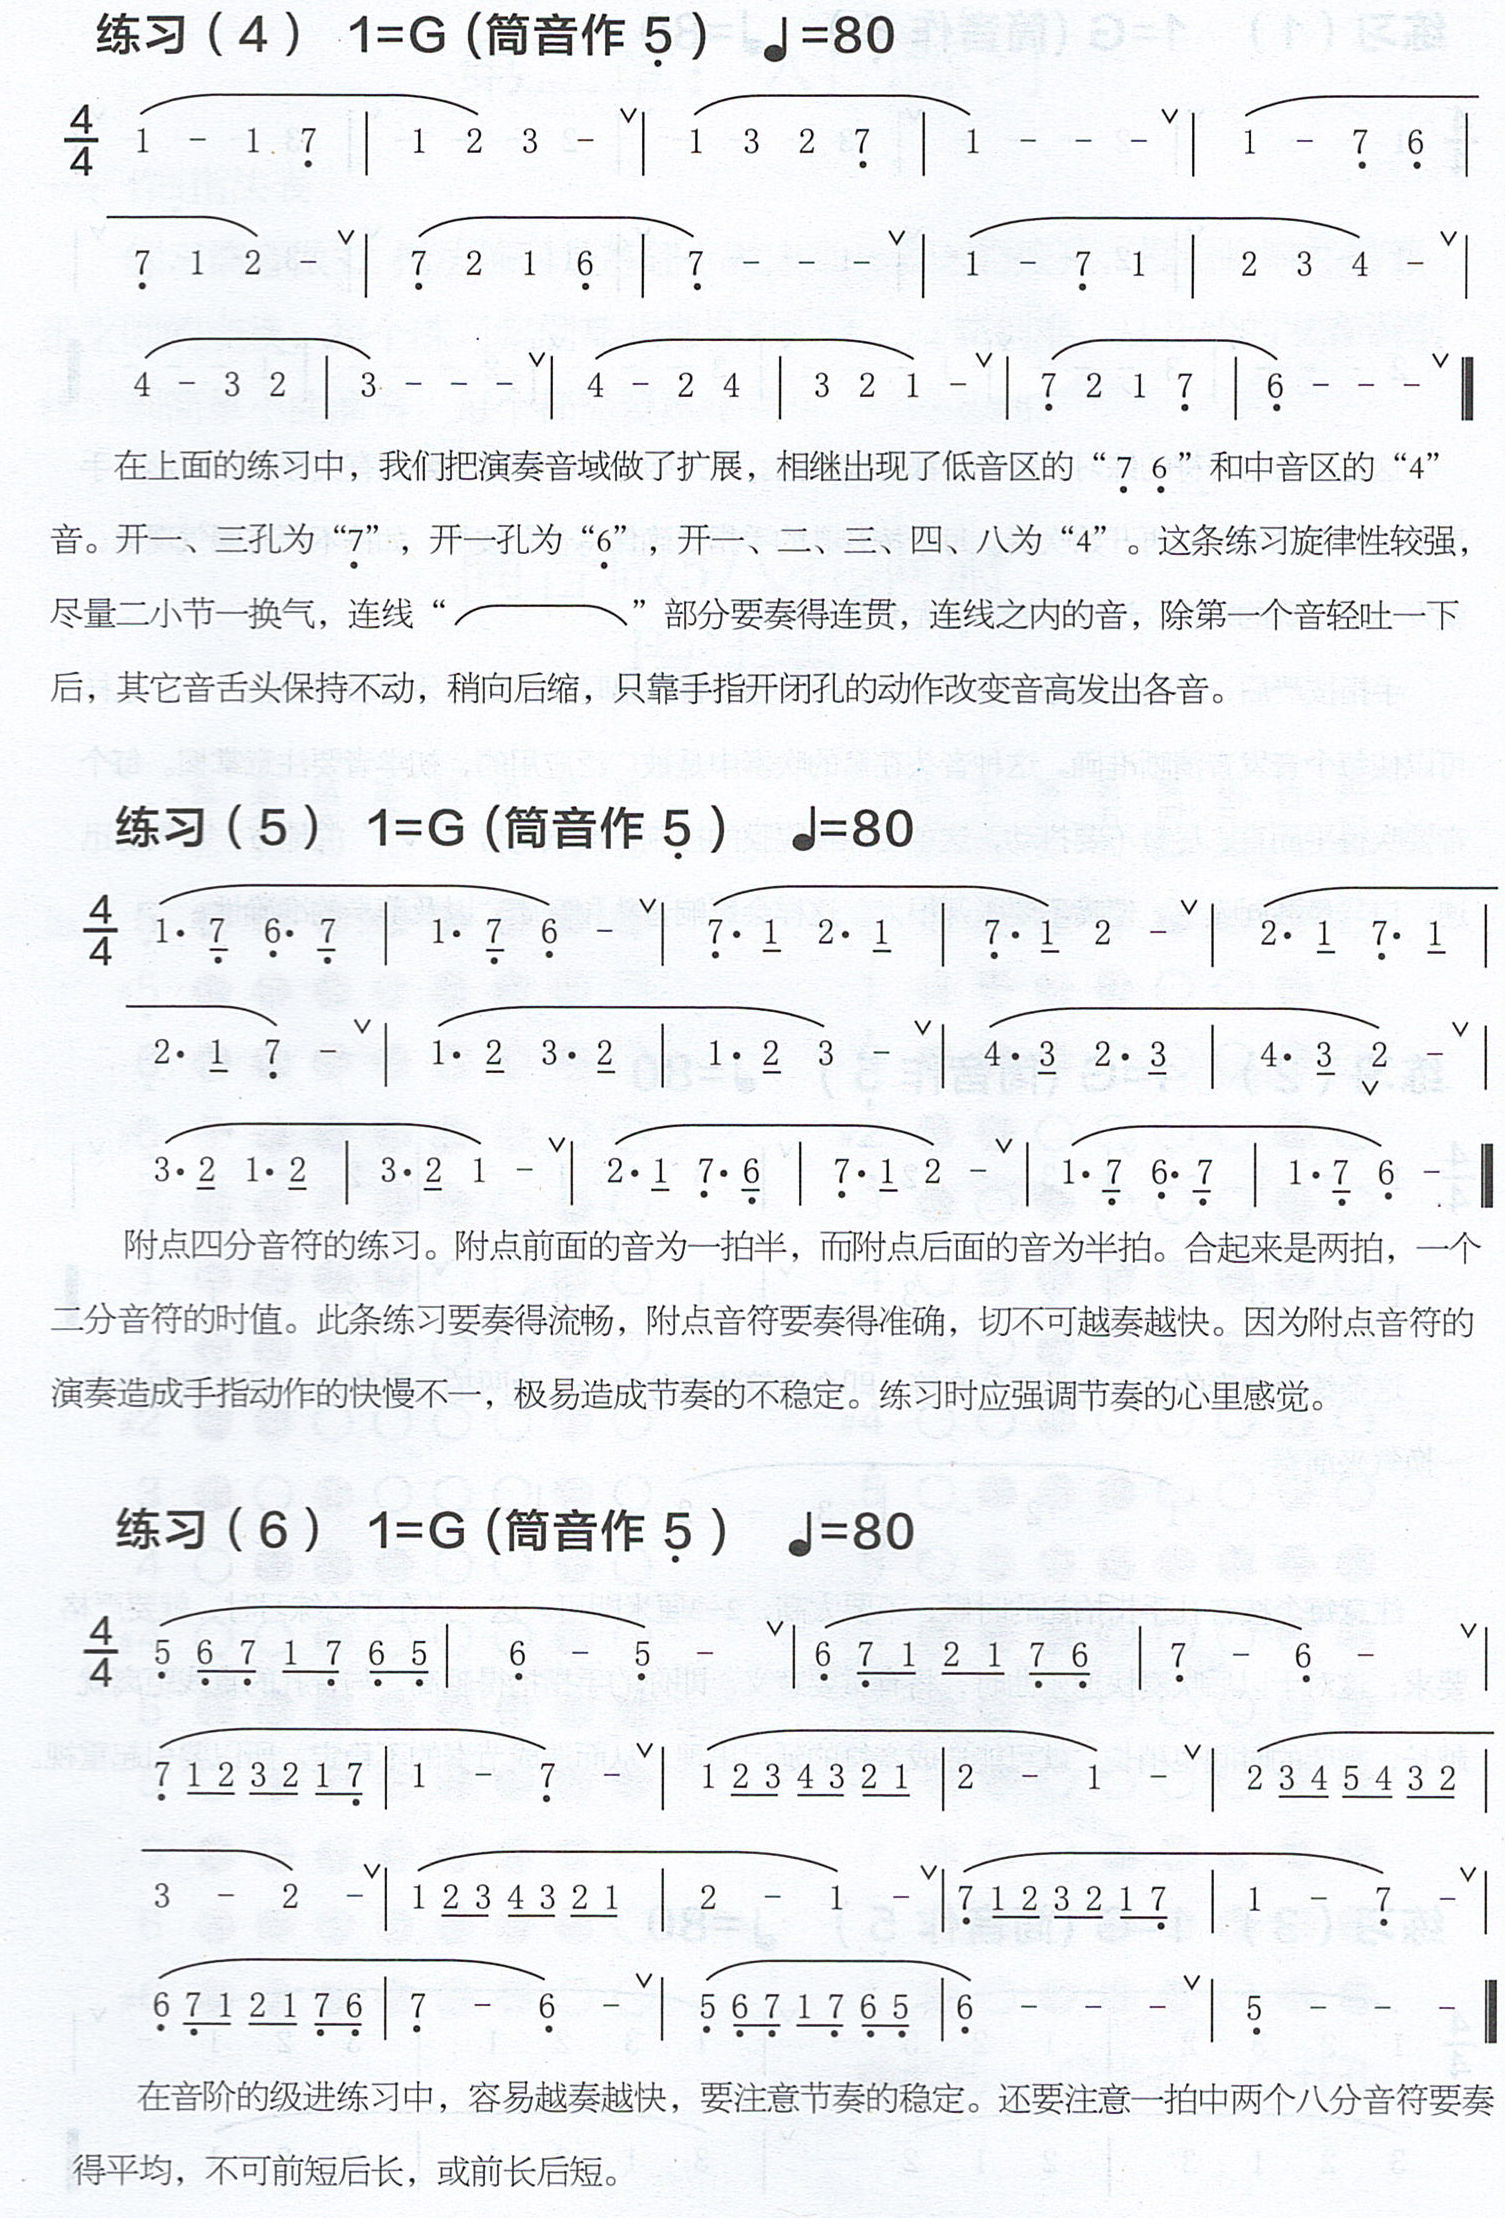
\includegraphics[height=\textheight]{dongxiao/Scan 2.jpeg}

\section{练习(7,8阿里郎,9欢乐女神)1=G}
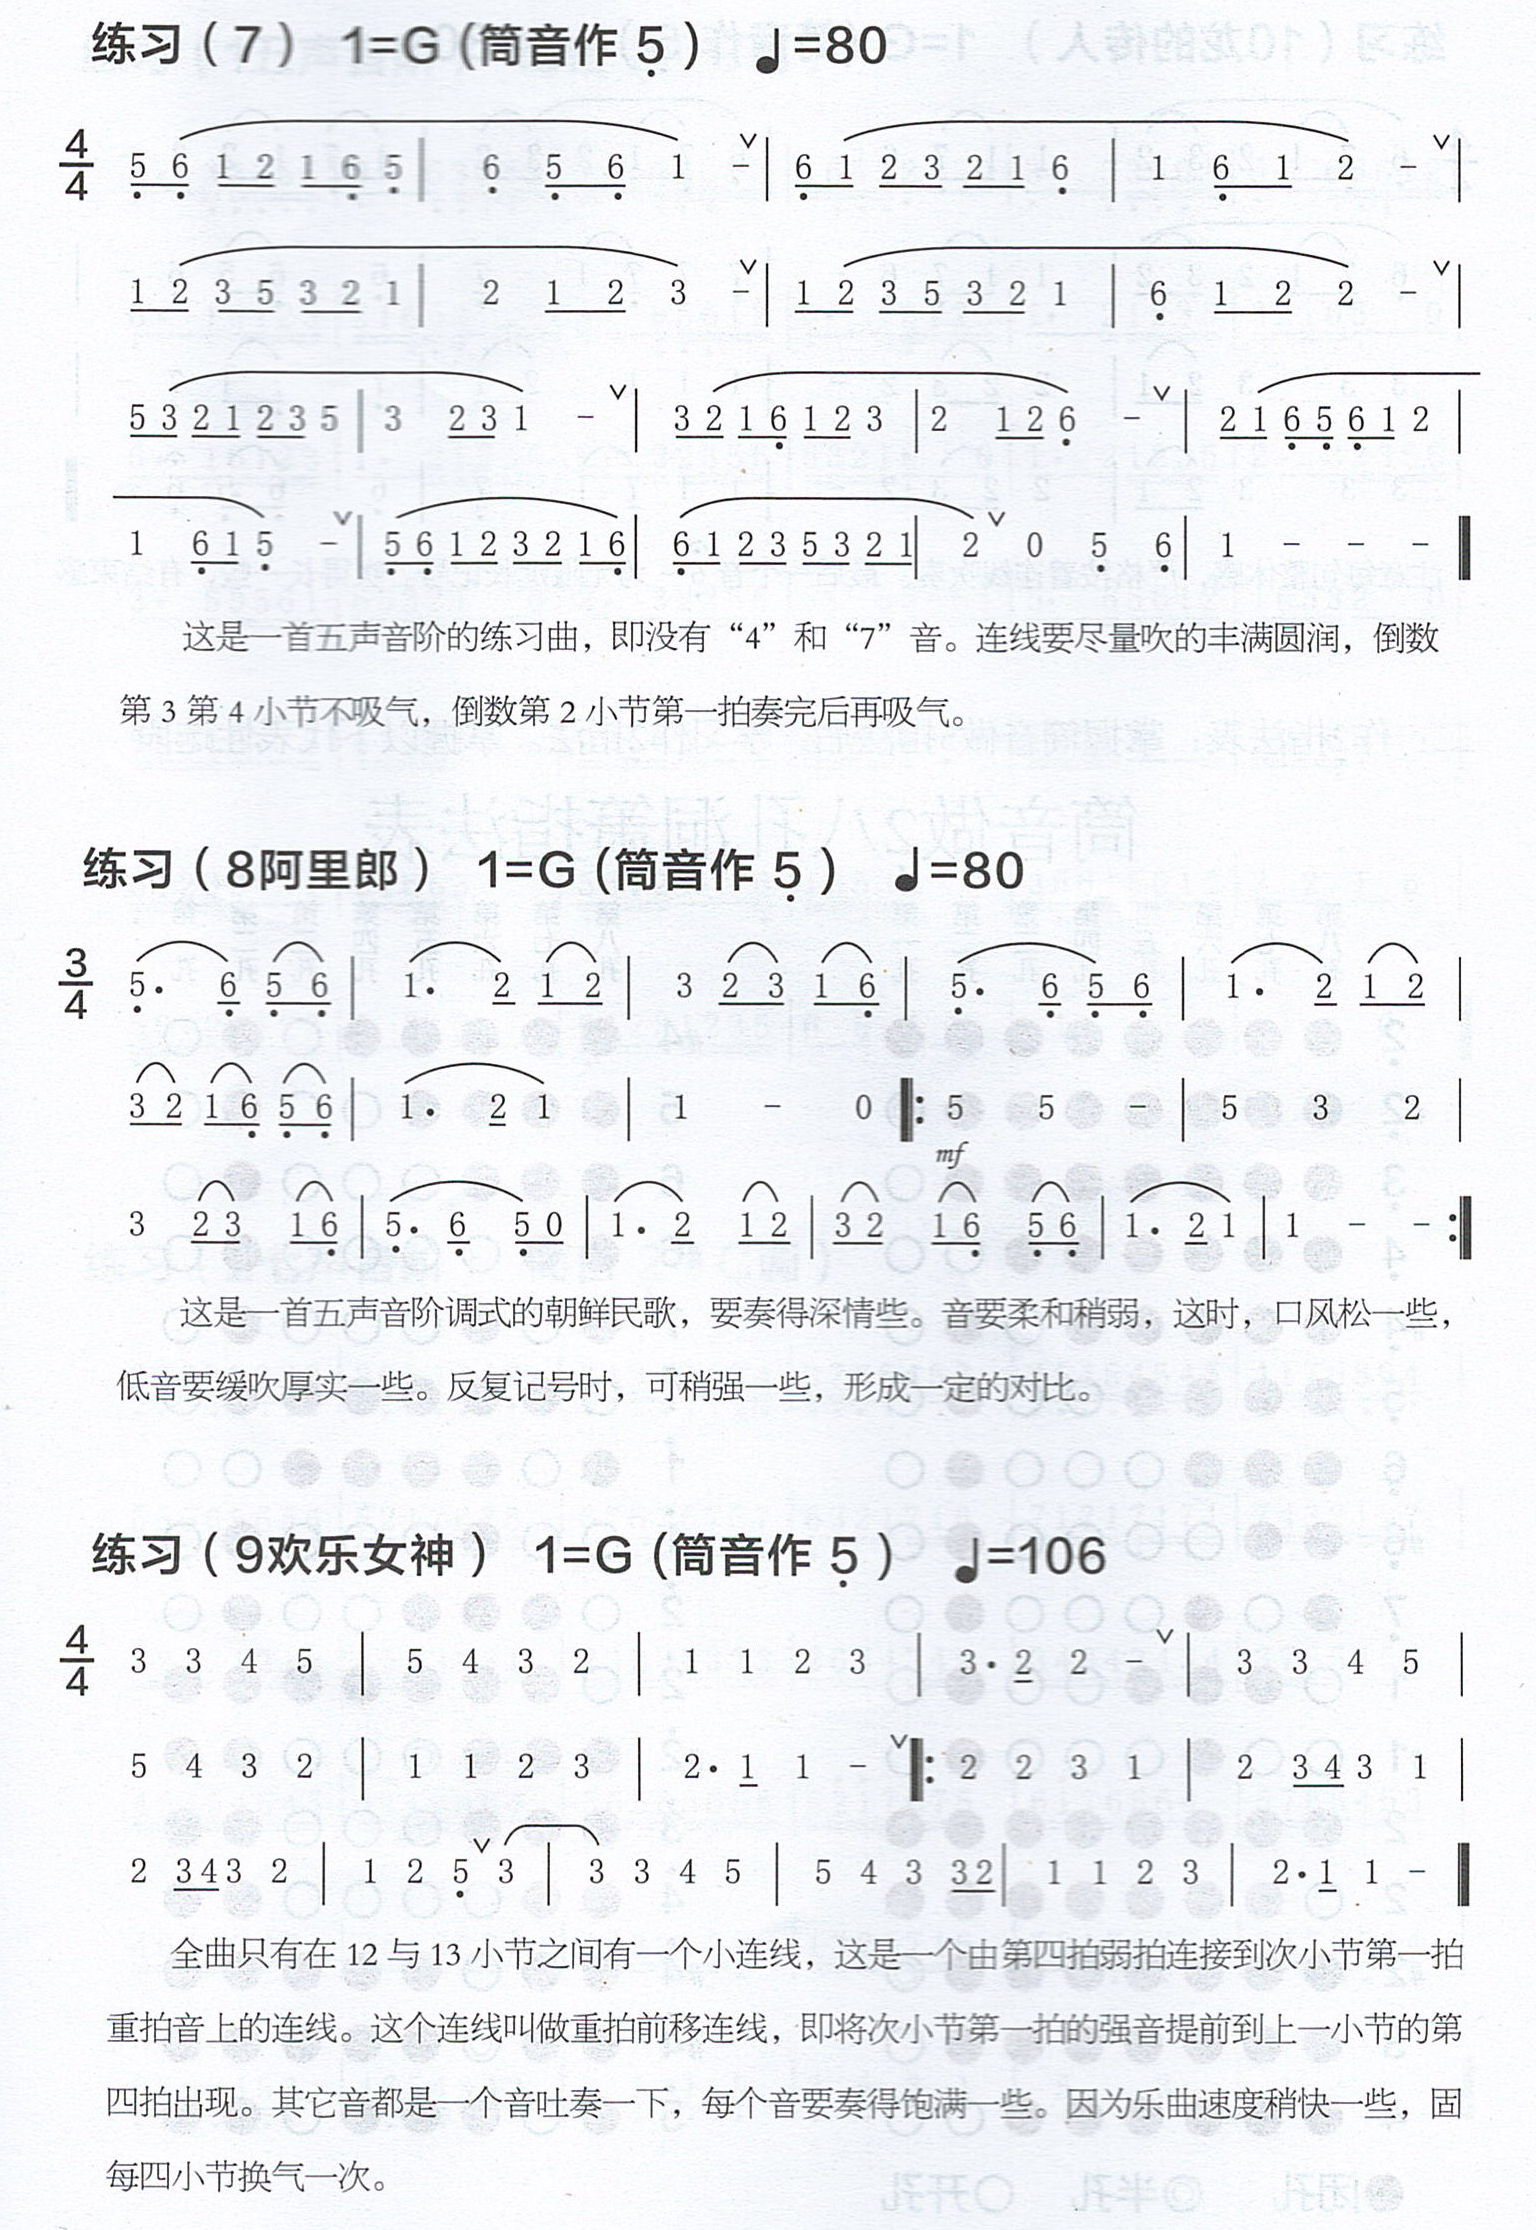
\includegraphics[height=\textheight]{dongxiao/Scan 3.jpeg}

\section{练习(10龙的传人)1=G}
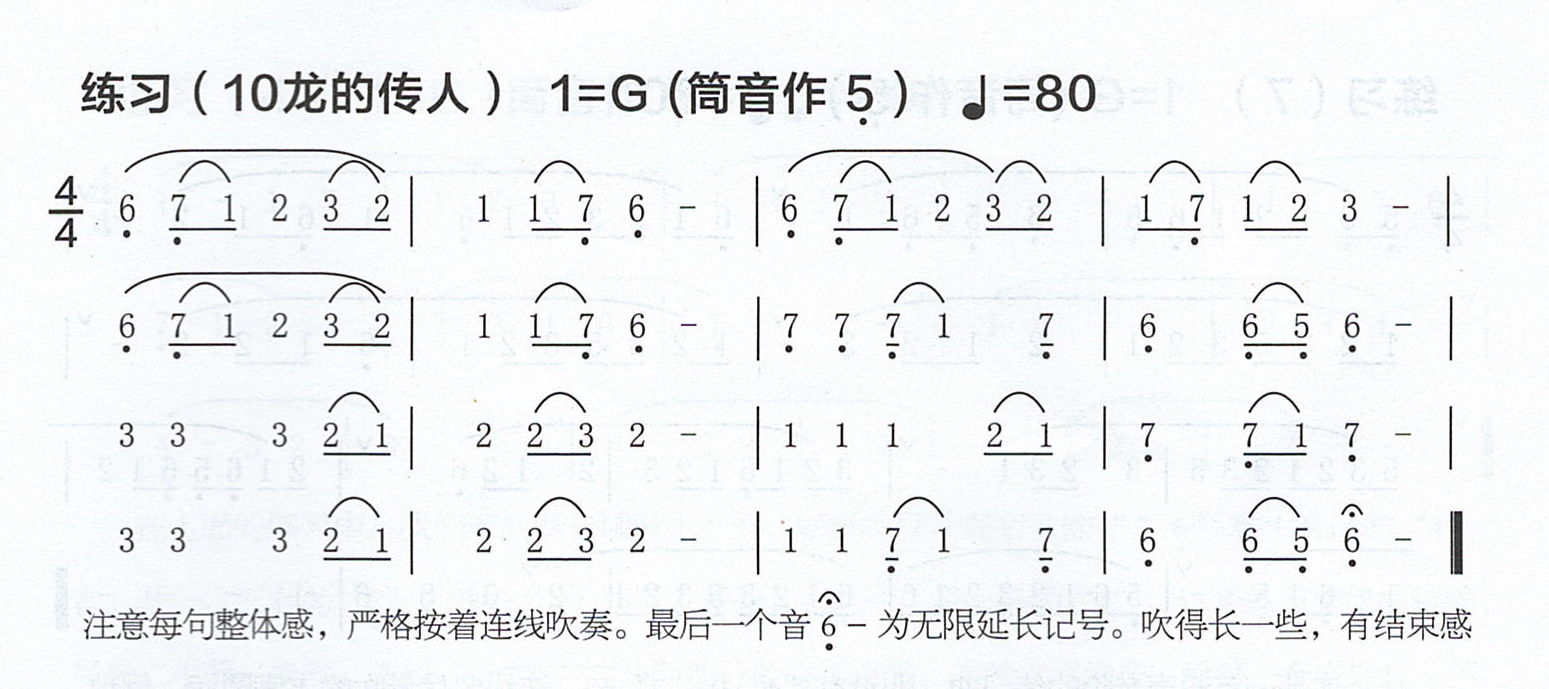
\includegraphics[width=\textwidth]{dongxiao/Scan 4.jpeg}

\chapter{筒音做‘低音2’}
\section{指法表}
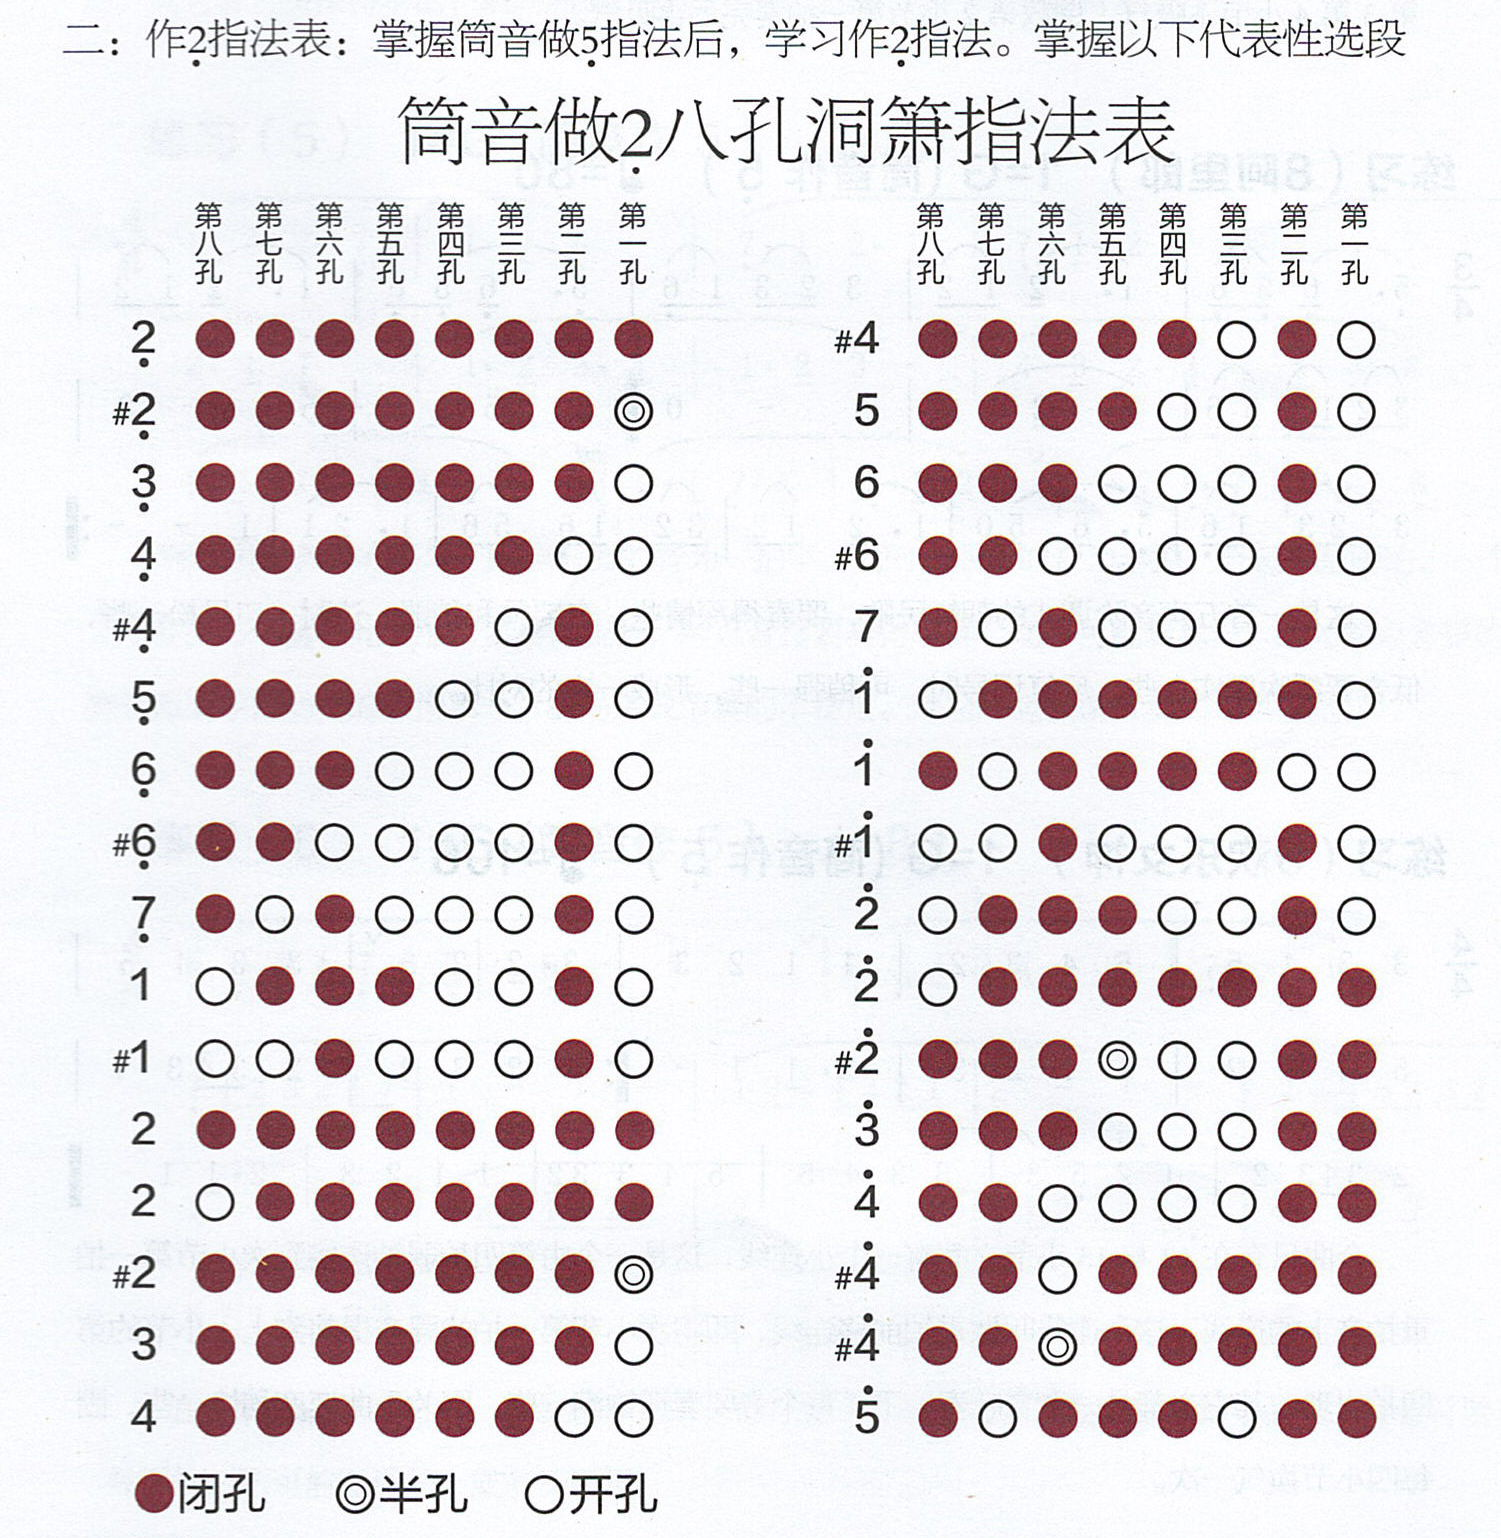
\includegraphics[width=\textwidth]{dongxiao/Scan 4.1.jpeg}

\section{练习(1-2)C调}
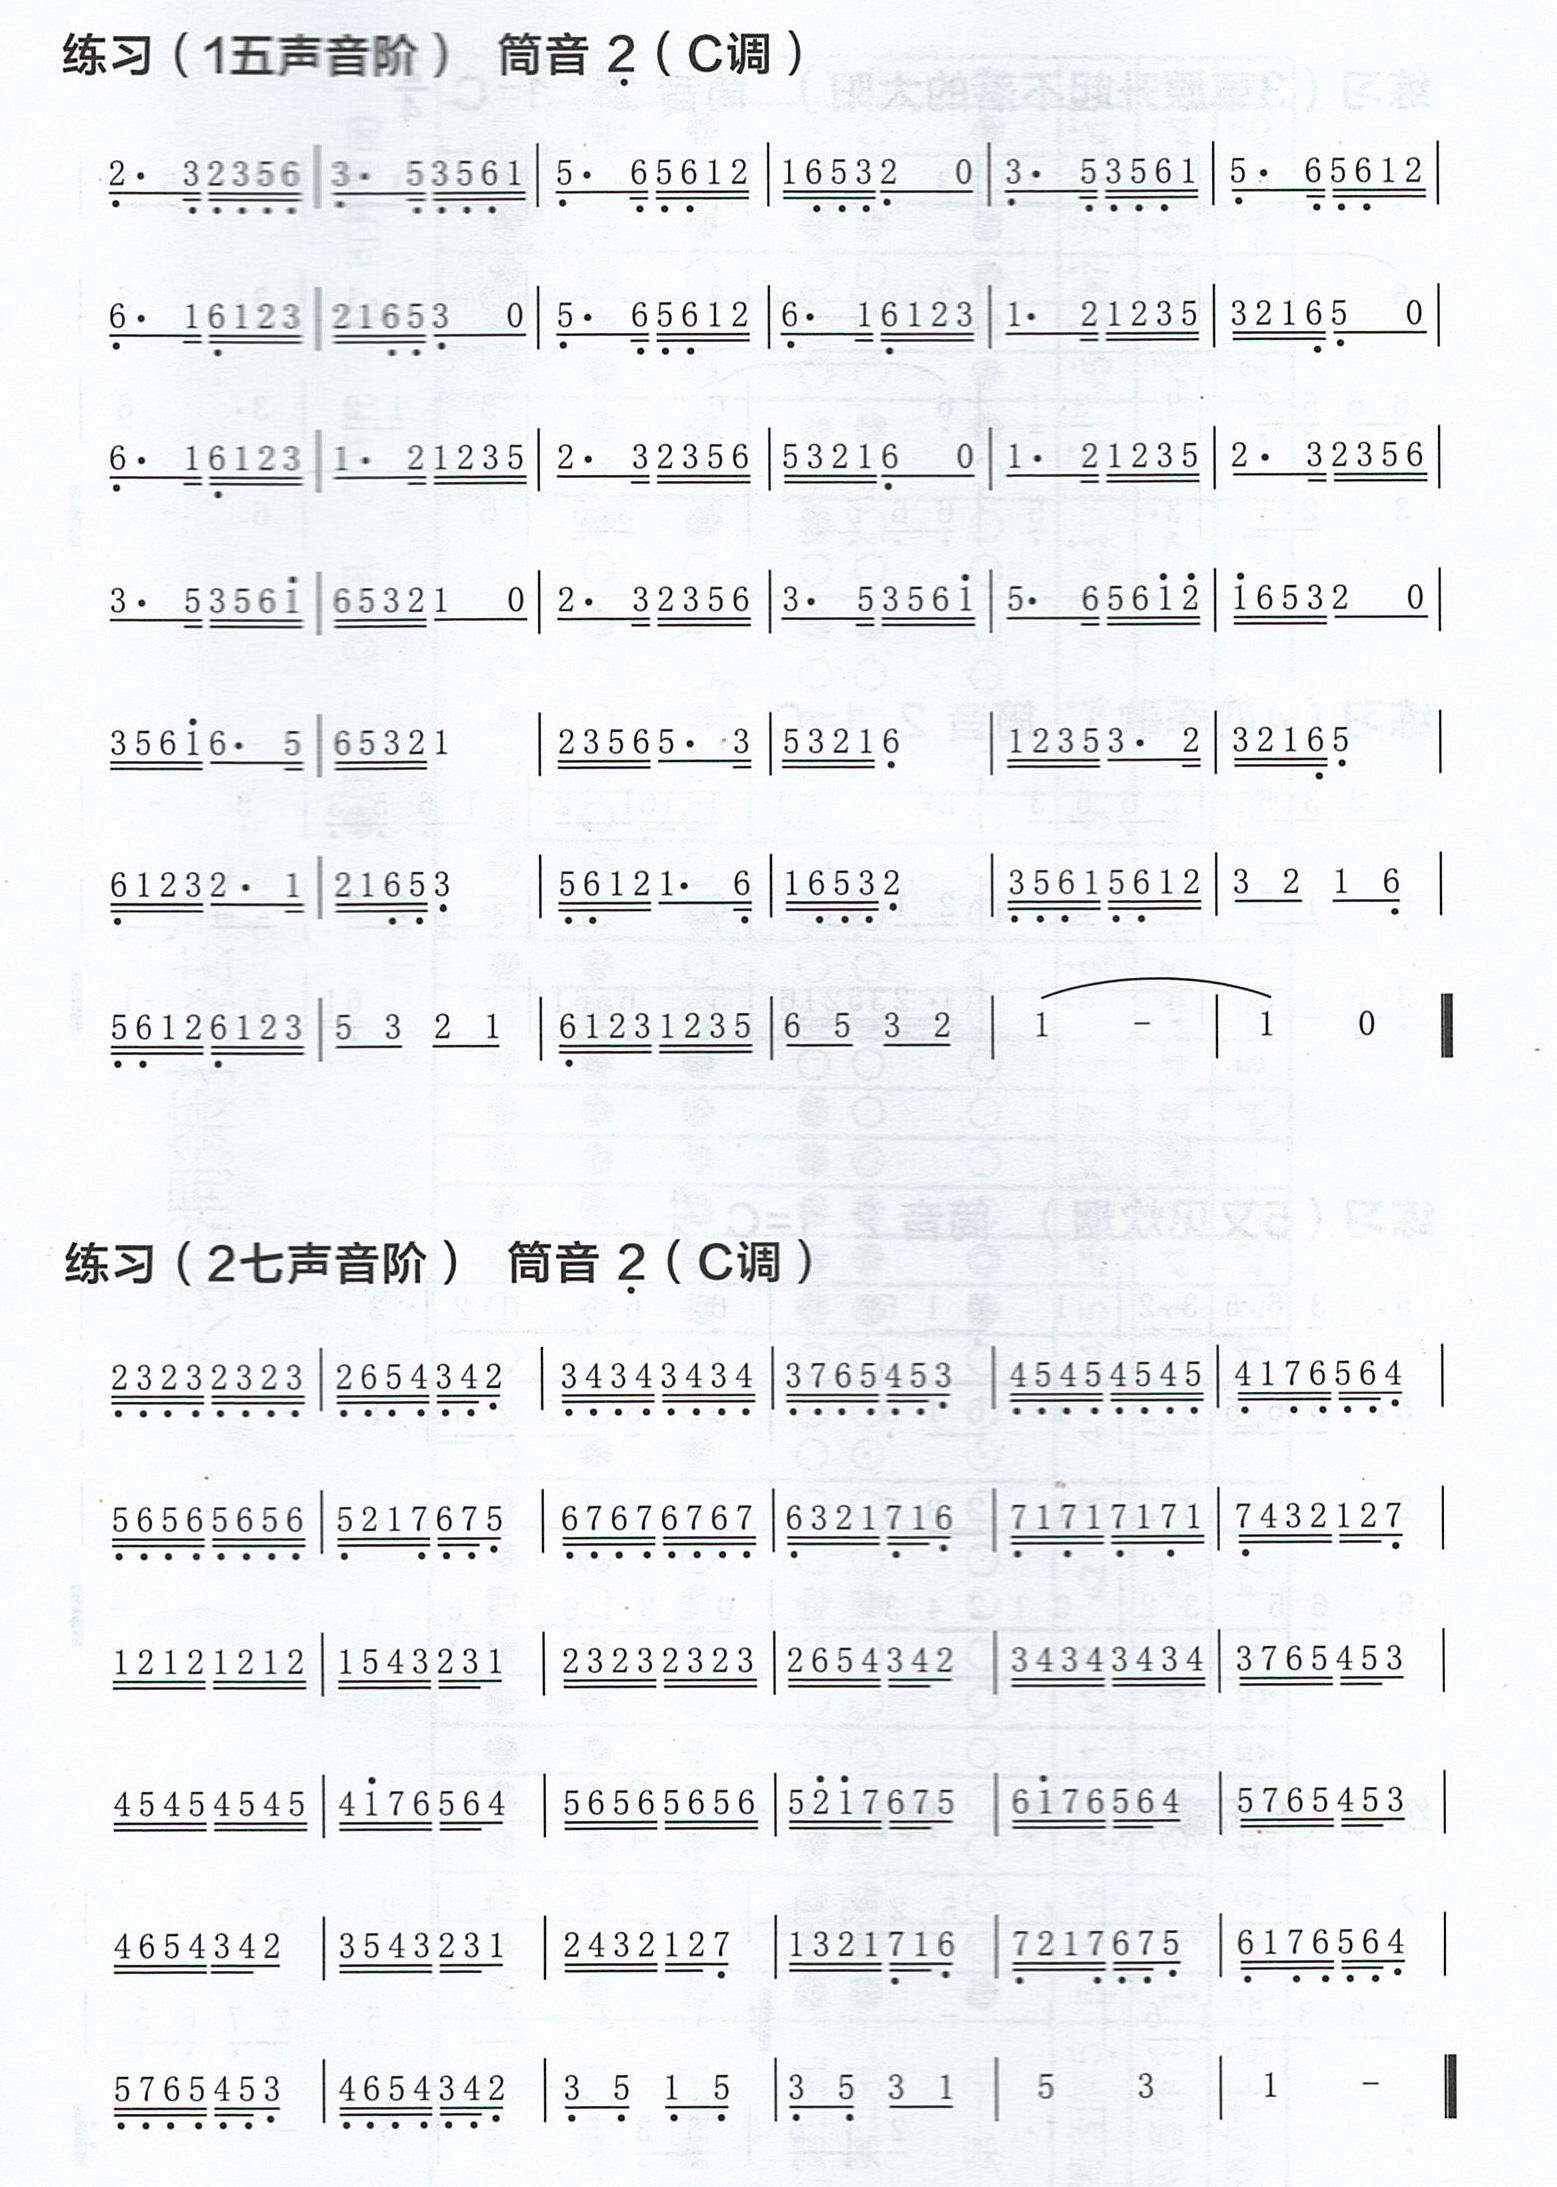
\includegraphics[height=\textheight]{dongxiao/Scan 5.jpeg}

\section{练习(3草原上升起不落的太阳2/4,4四季歌2/4 5又见炊烟4/4 6沂蒙山小调3/4)1=C}
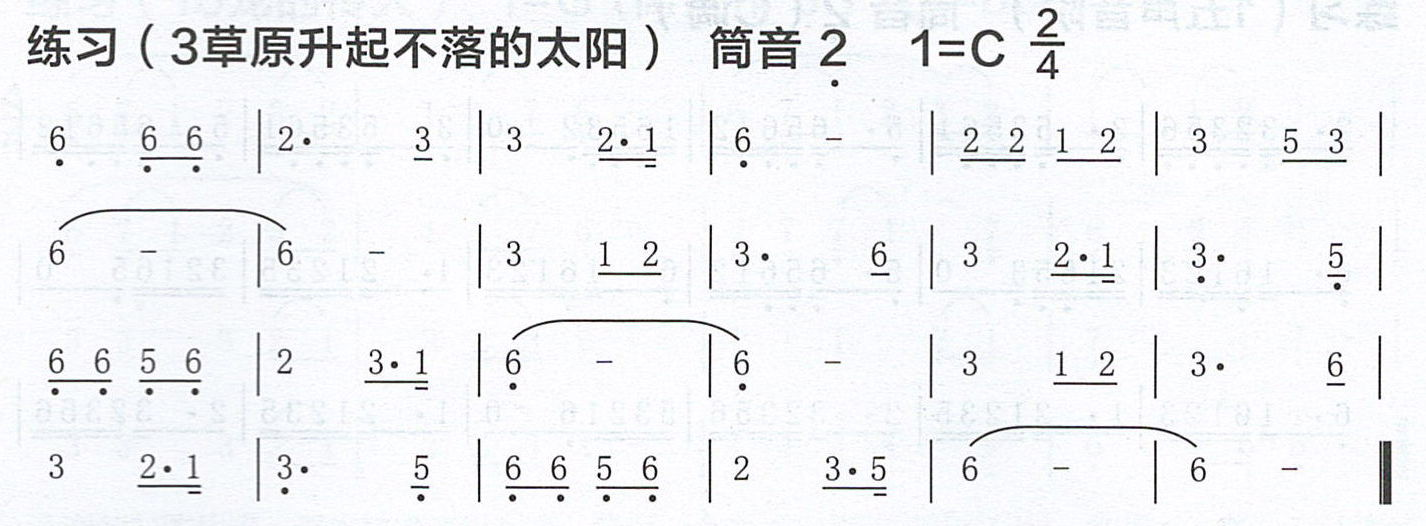
\includegraphics[height=\textheight]{dongxiao/Scan 6.jpeg}

\chapter{技巧练习}
\section{长音练习(1全按作低音5,2全按作低音5)}
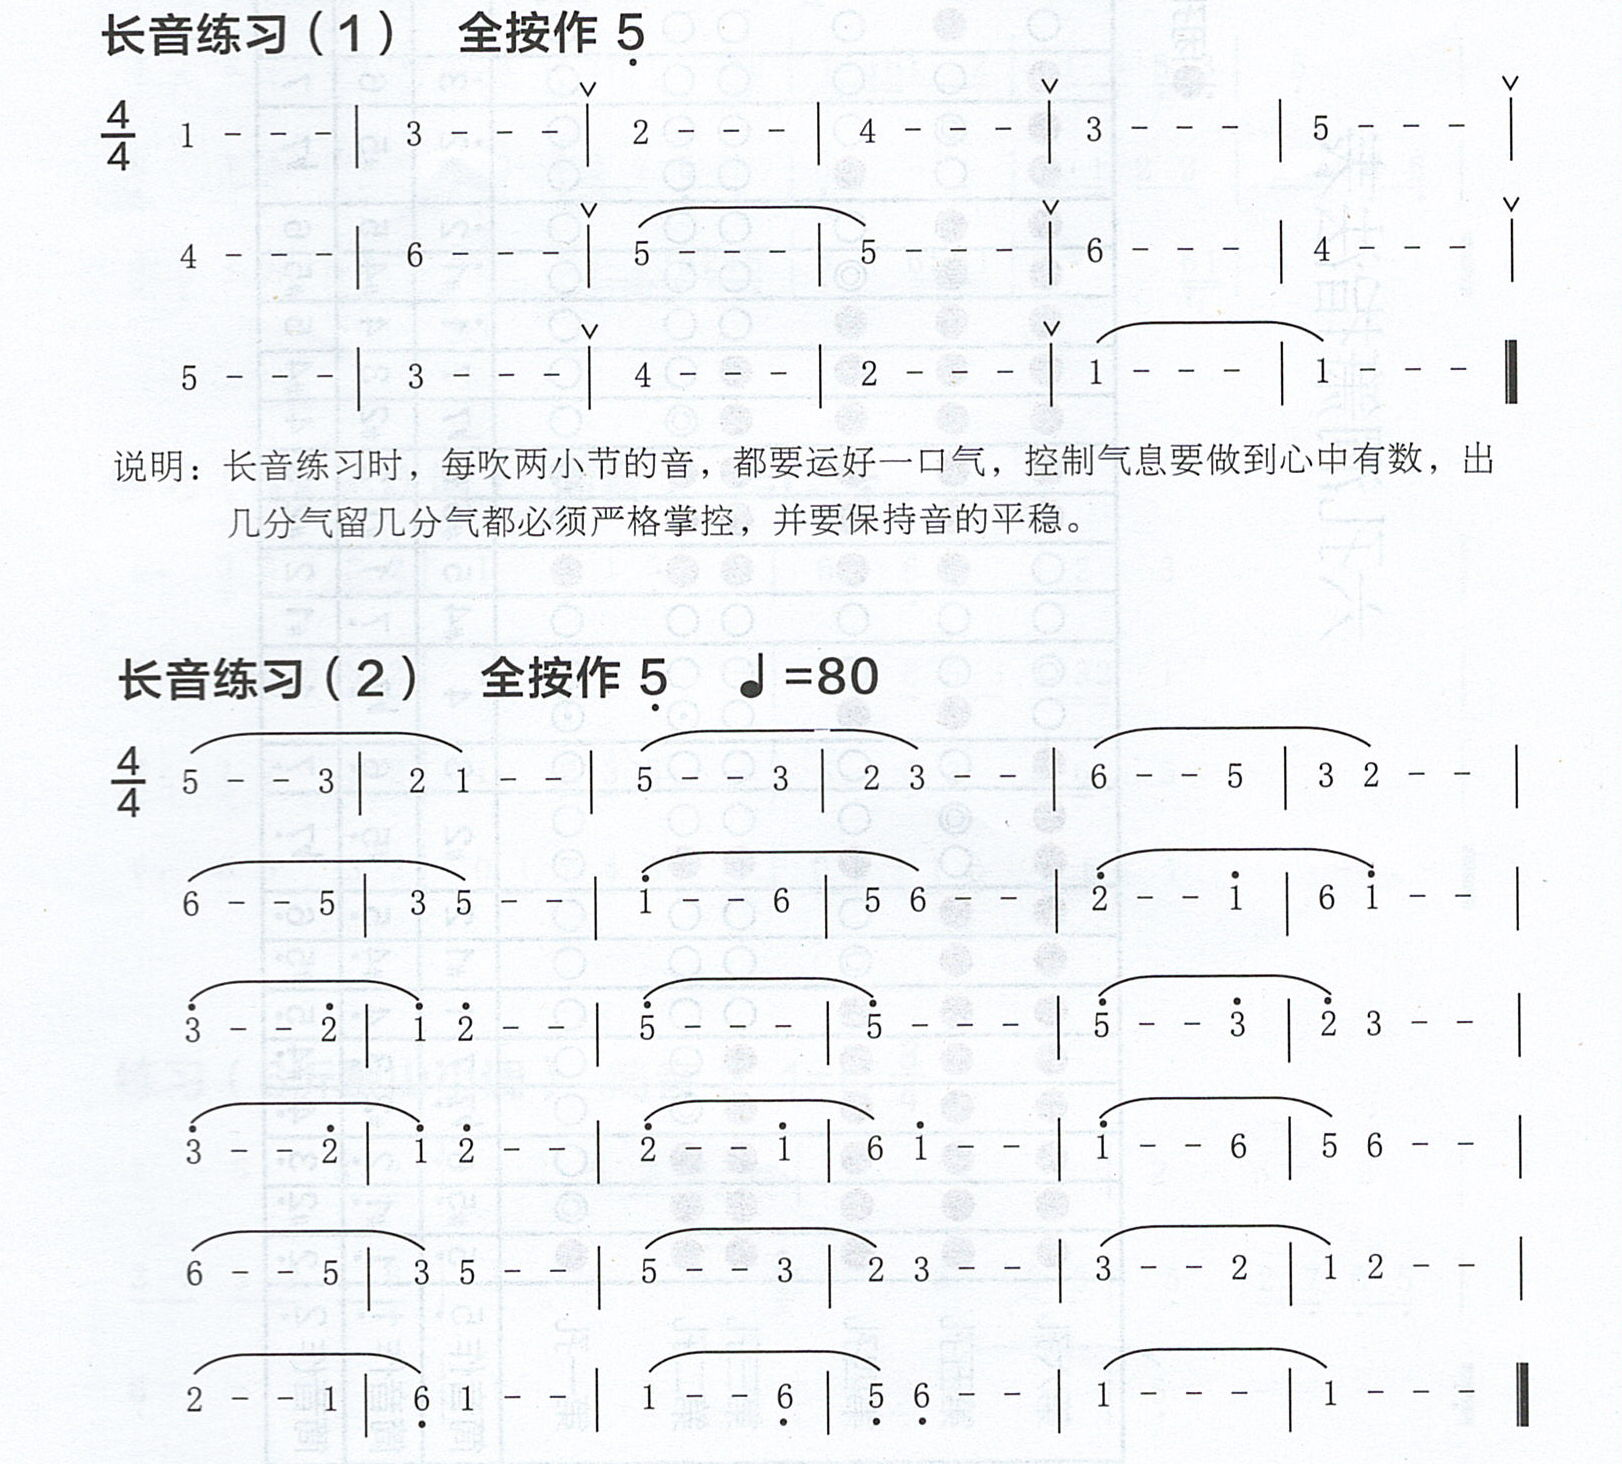
\includegraphics[width=\textwidth]{dongxiao/Scan 7.jpeg}

\section{气震音练习(1全按作低音2,2全按作低音2 牧歌)}
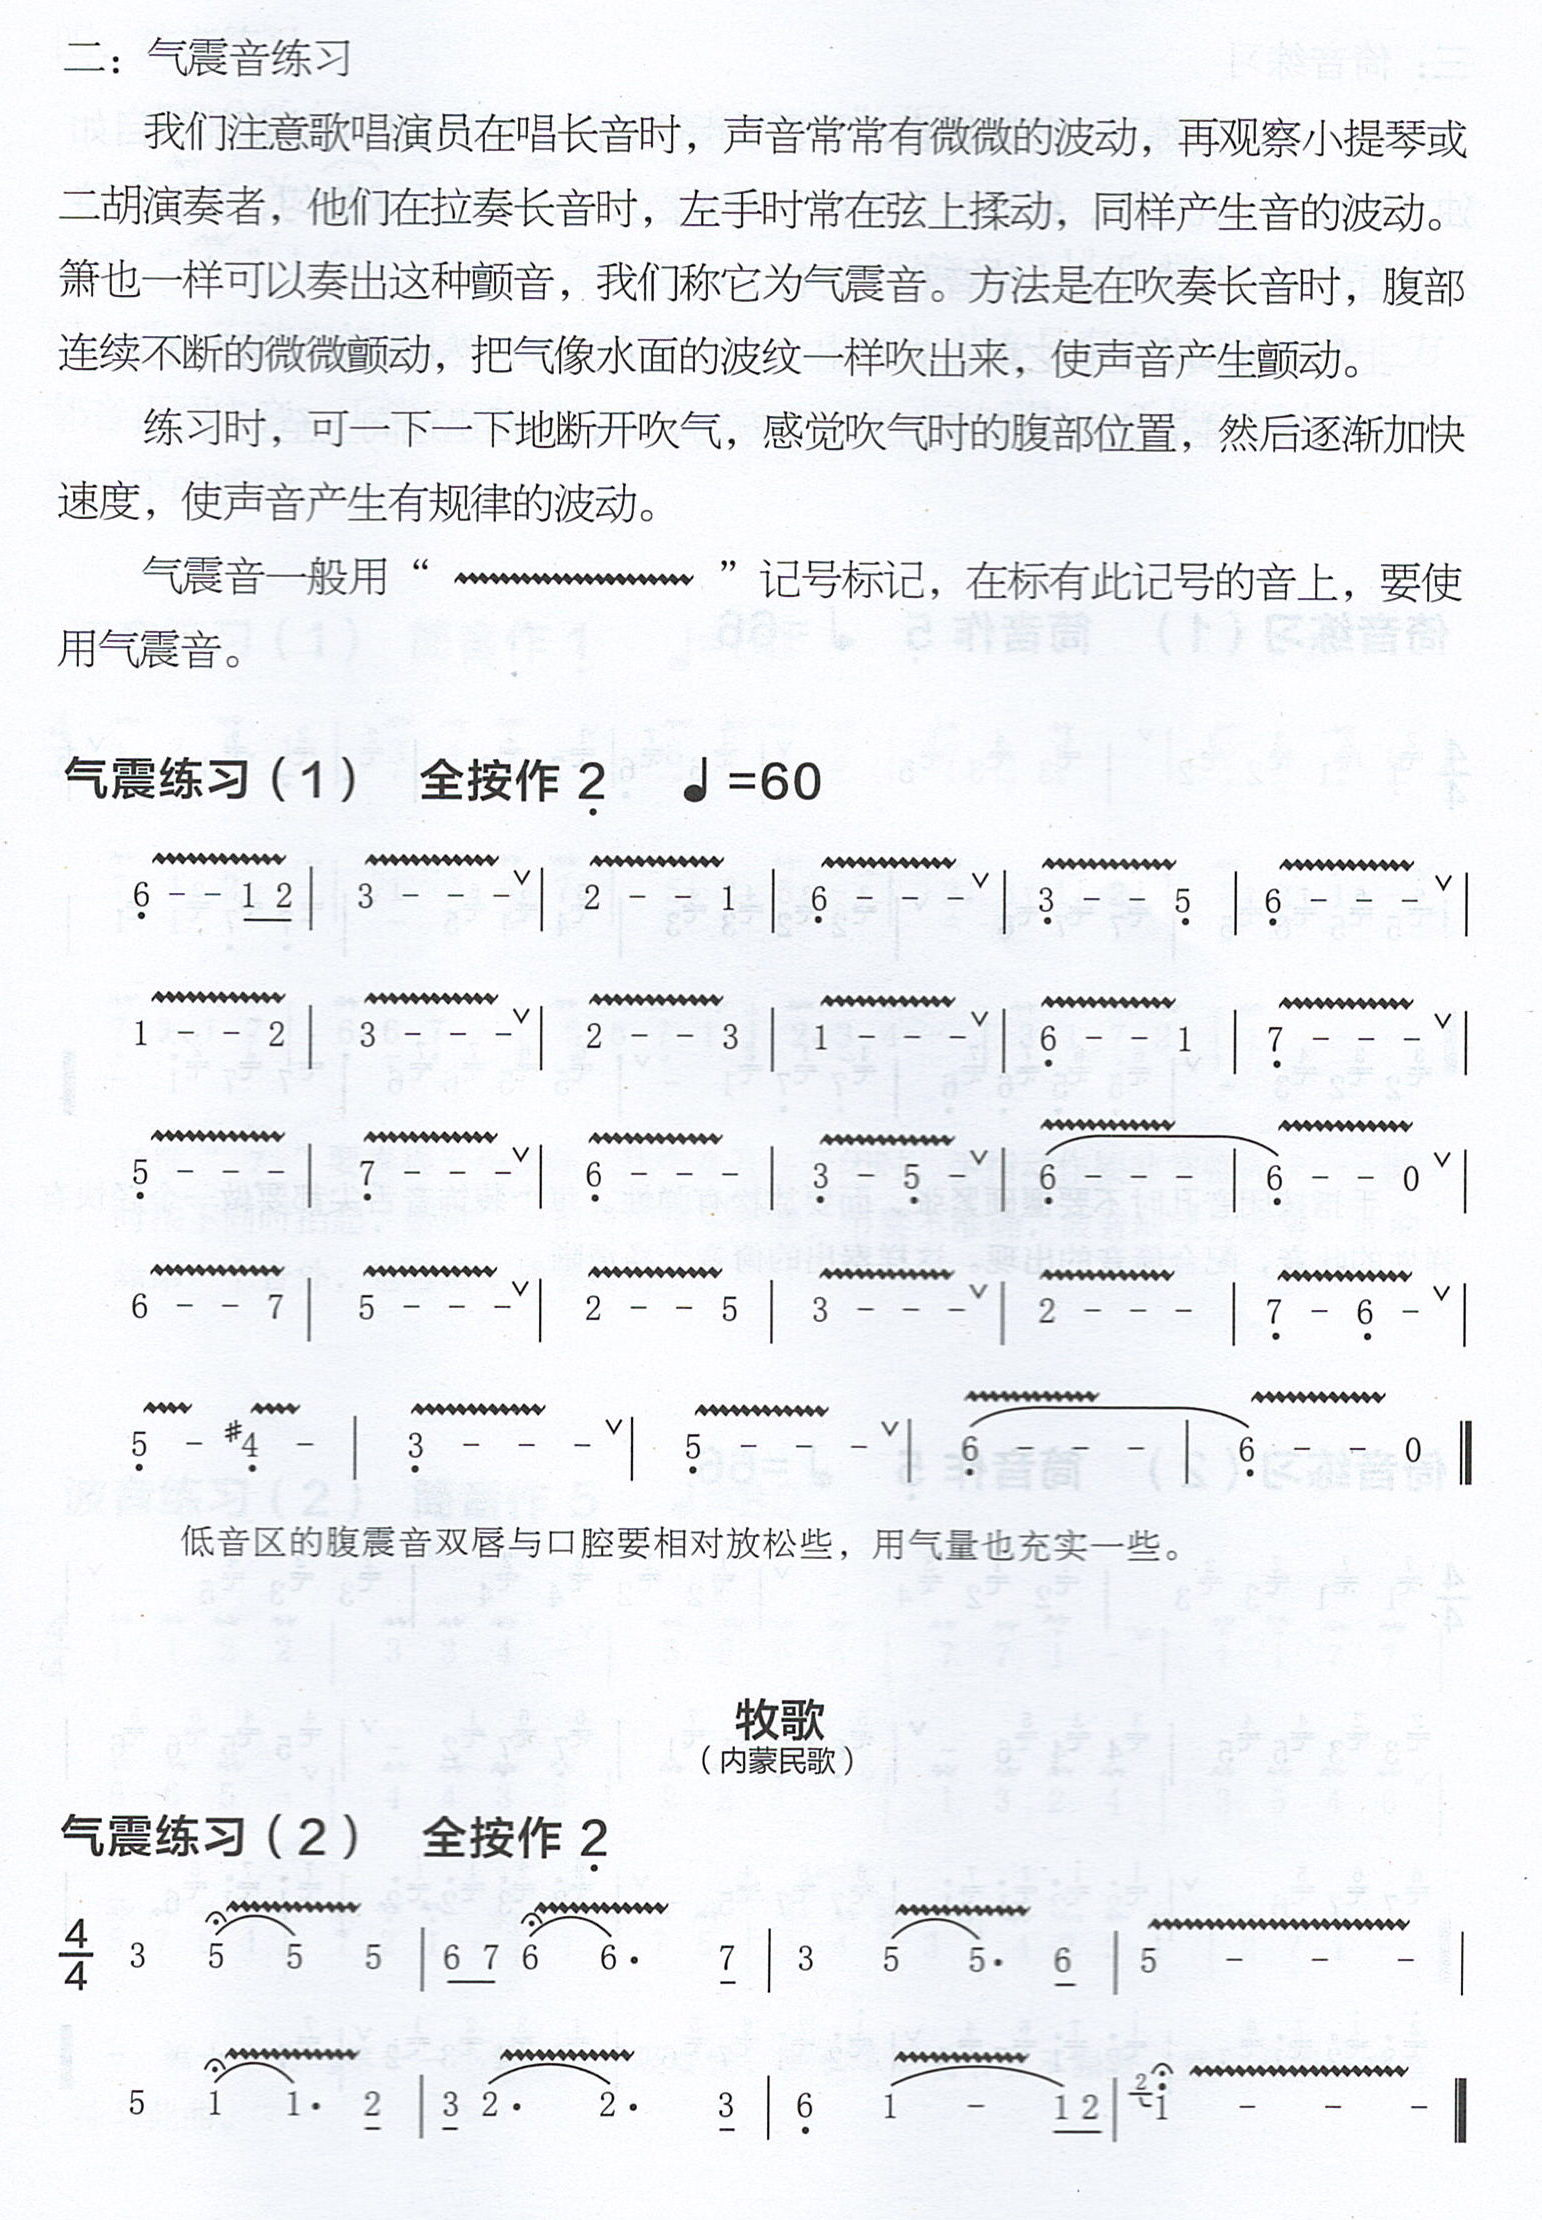
\includegraphics[height=\textheight]{dongxiao/Scan 8.jpeg}

\section{倚音练习(1全按作低音5,2全按作低音5)}
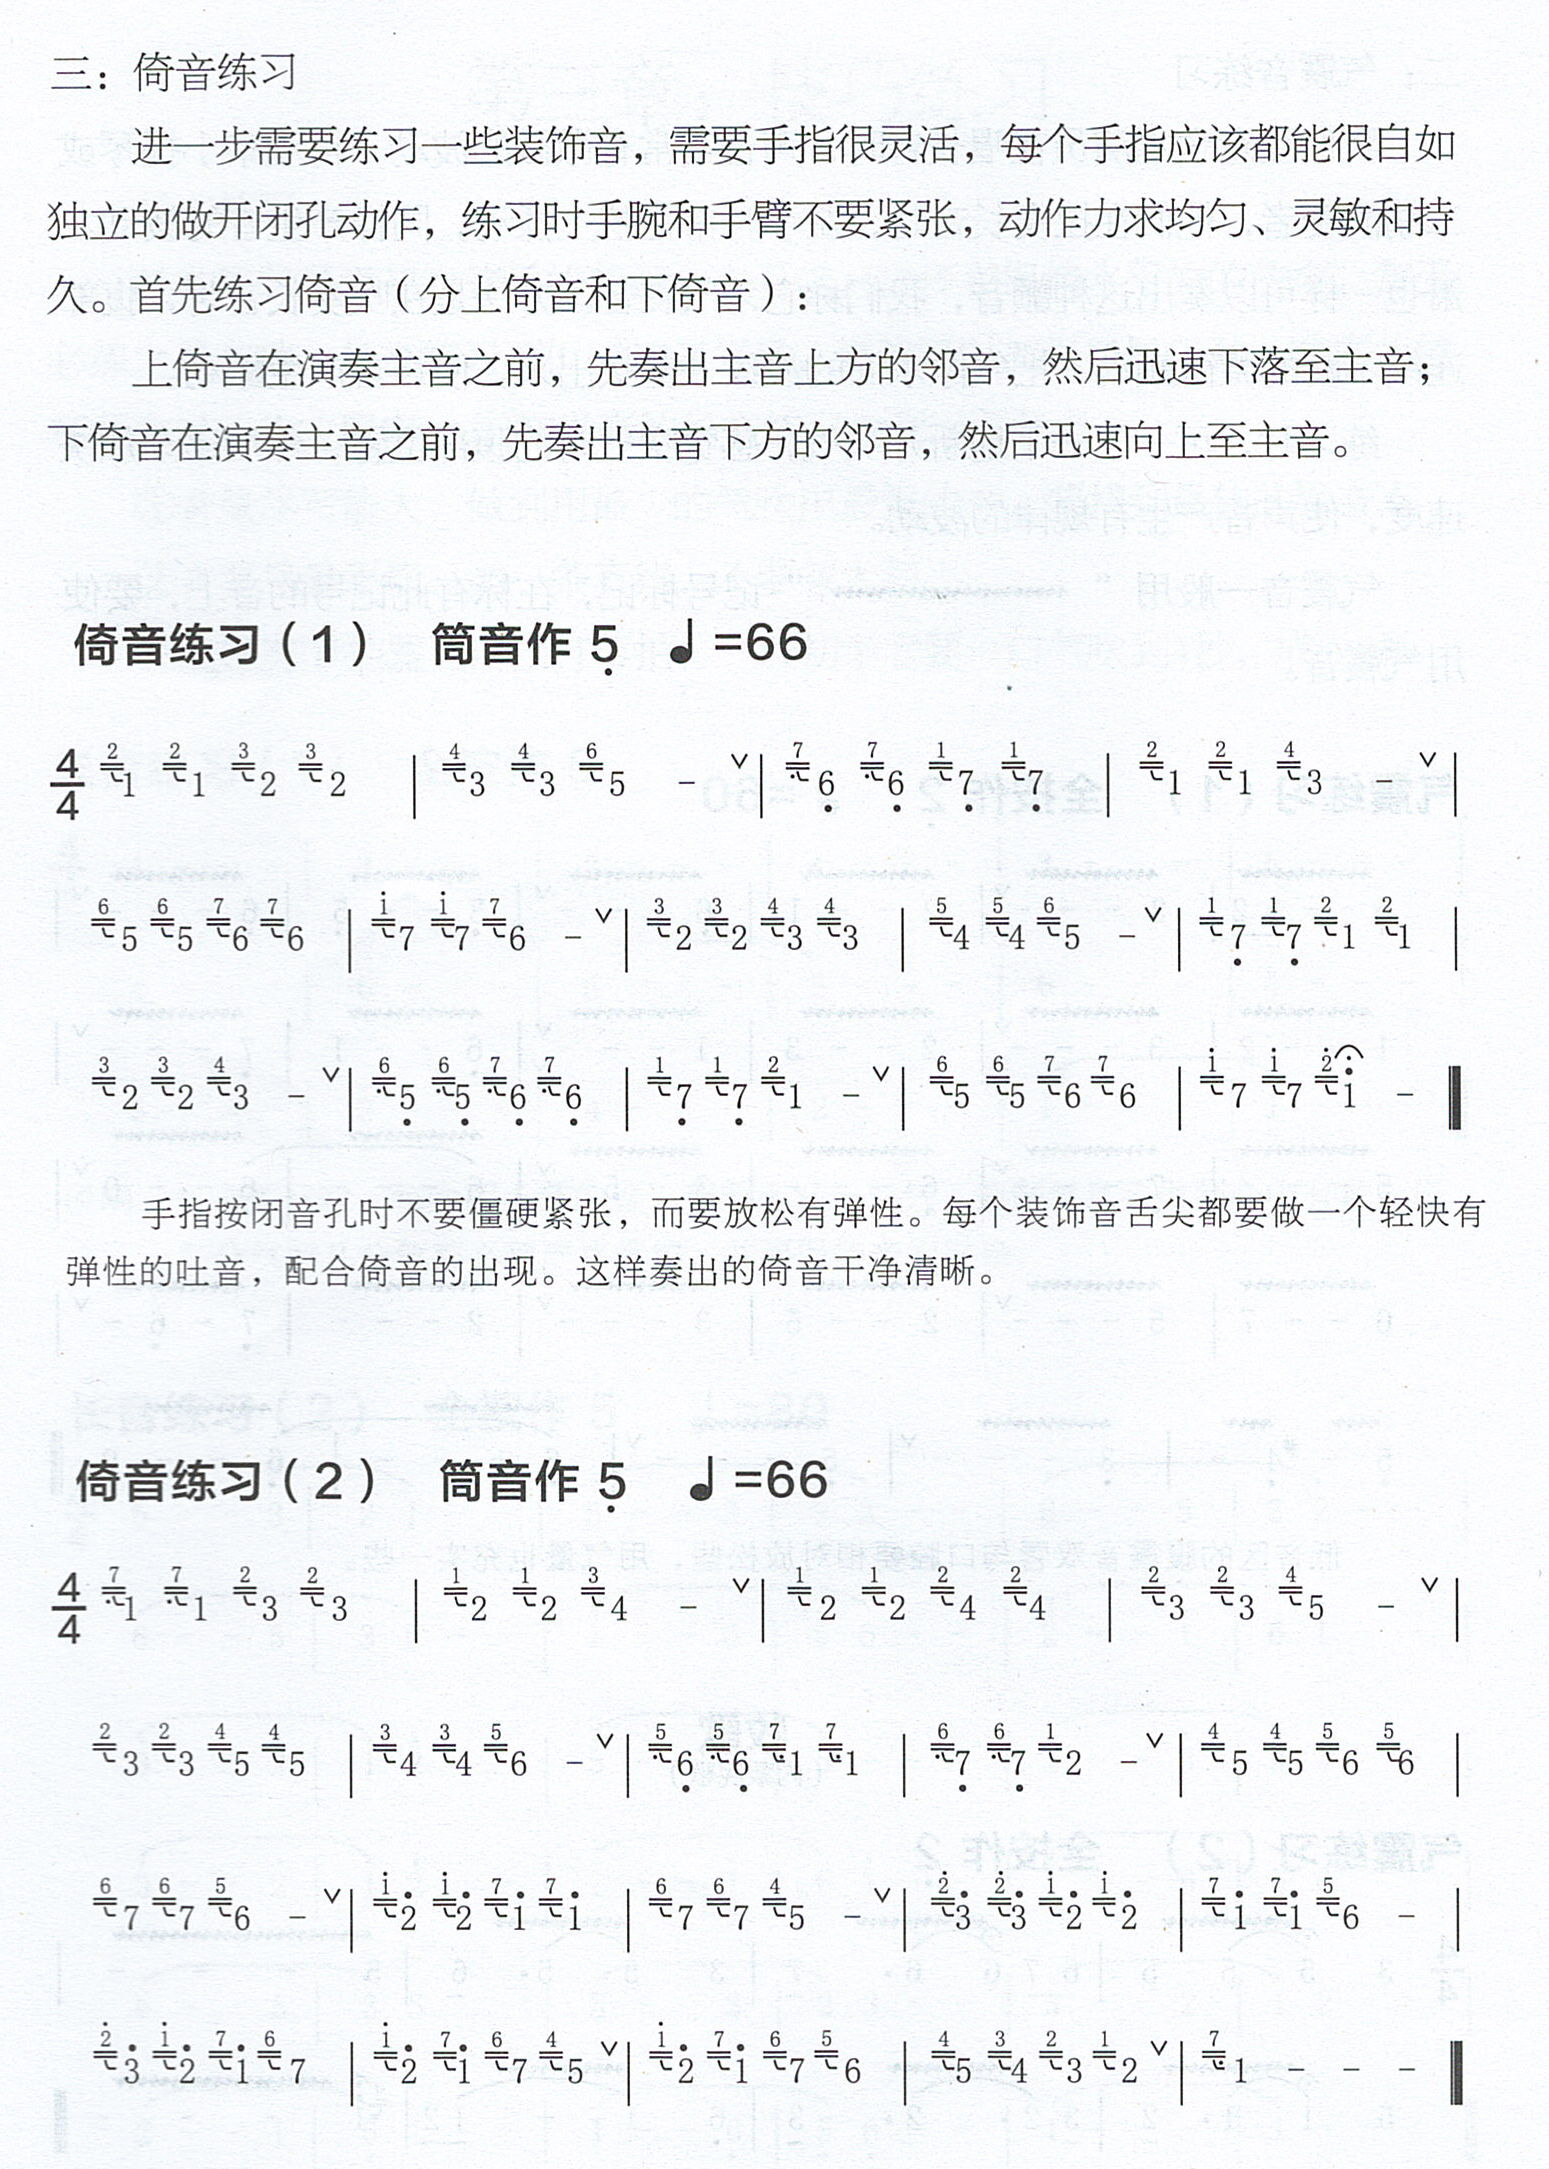
\includegraphics[height=\textheight]{dongxiao/Scan 9.jpeg}

\section{波音练习(1全按作低音1,2全按作低音5)}
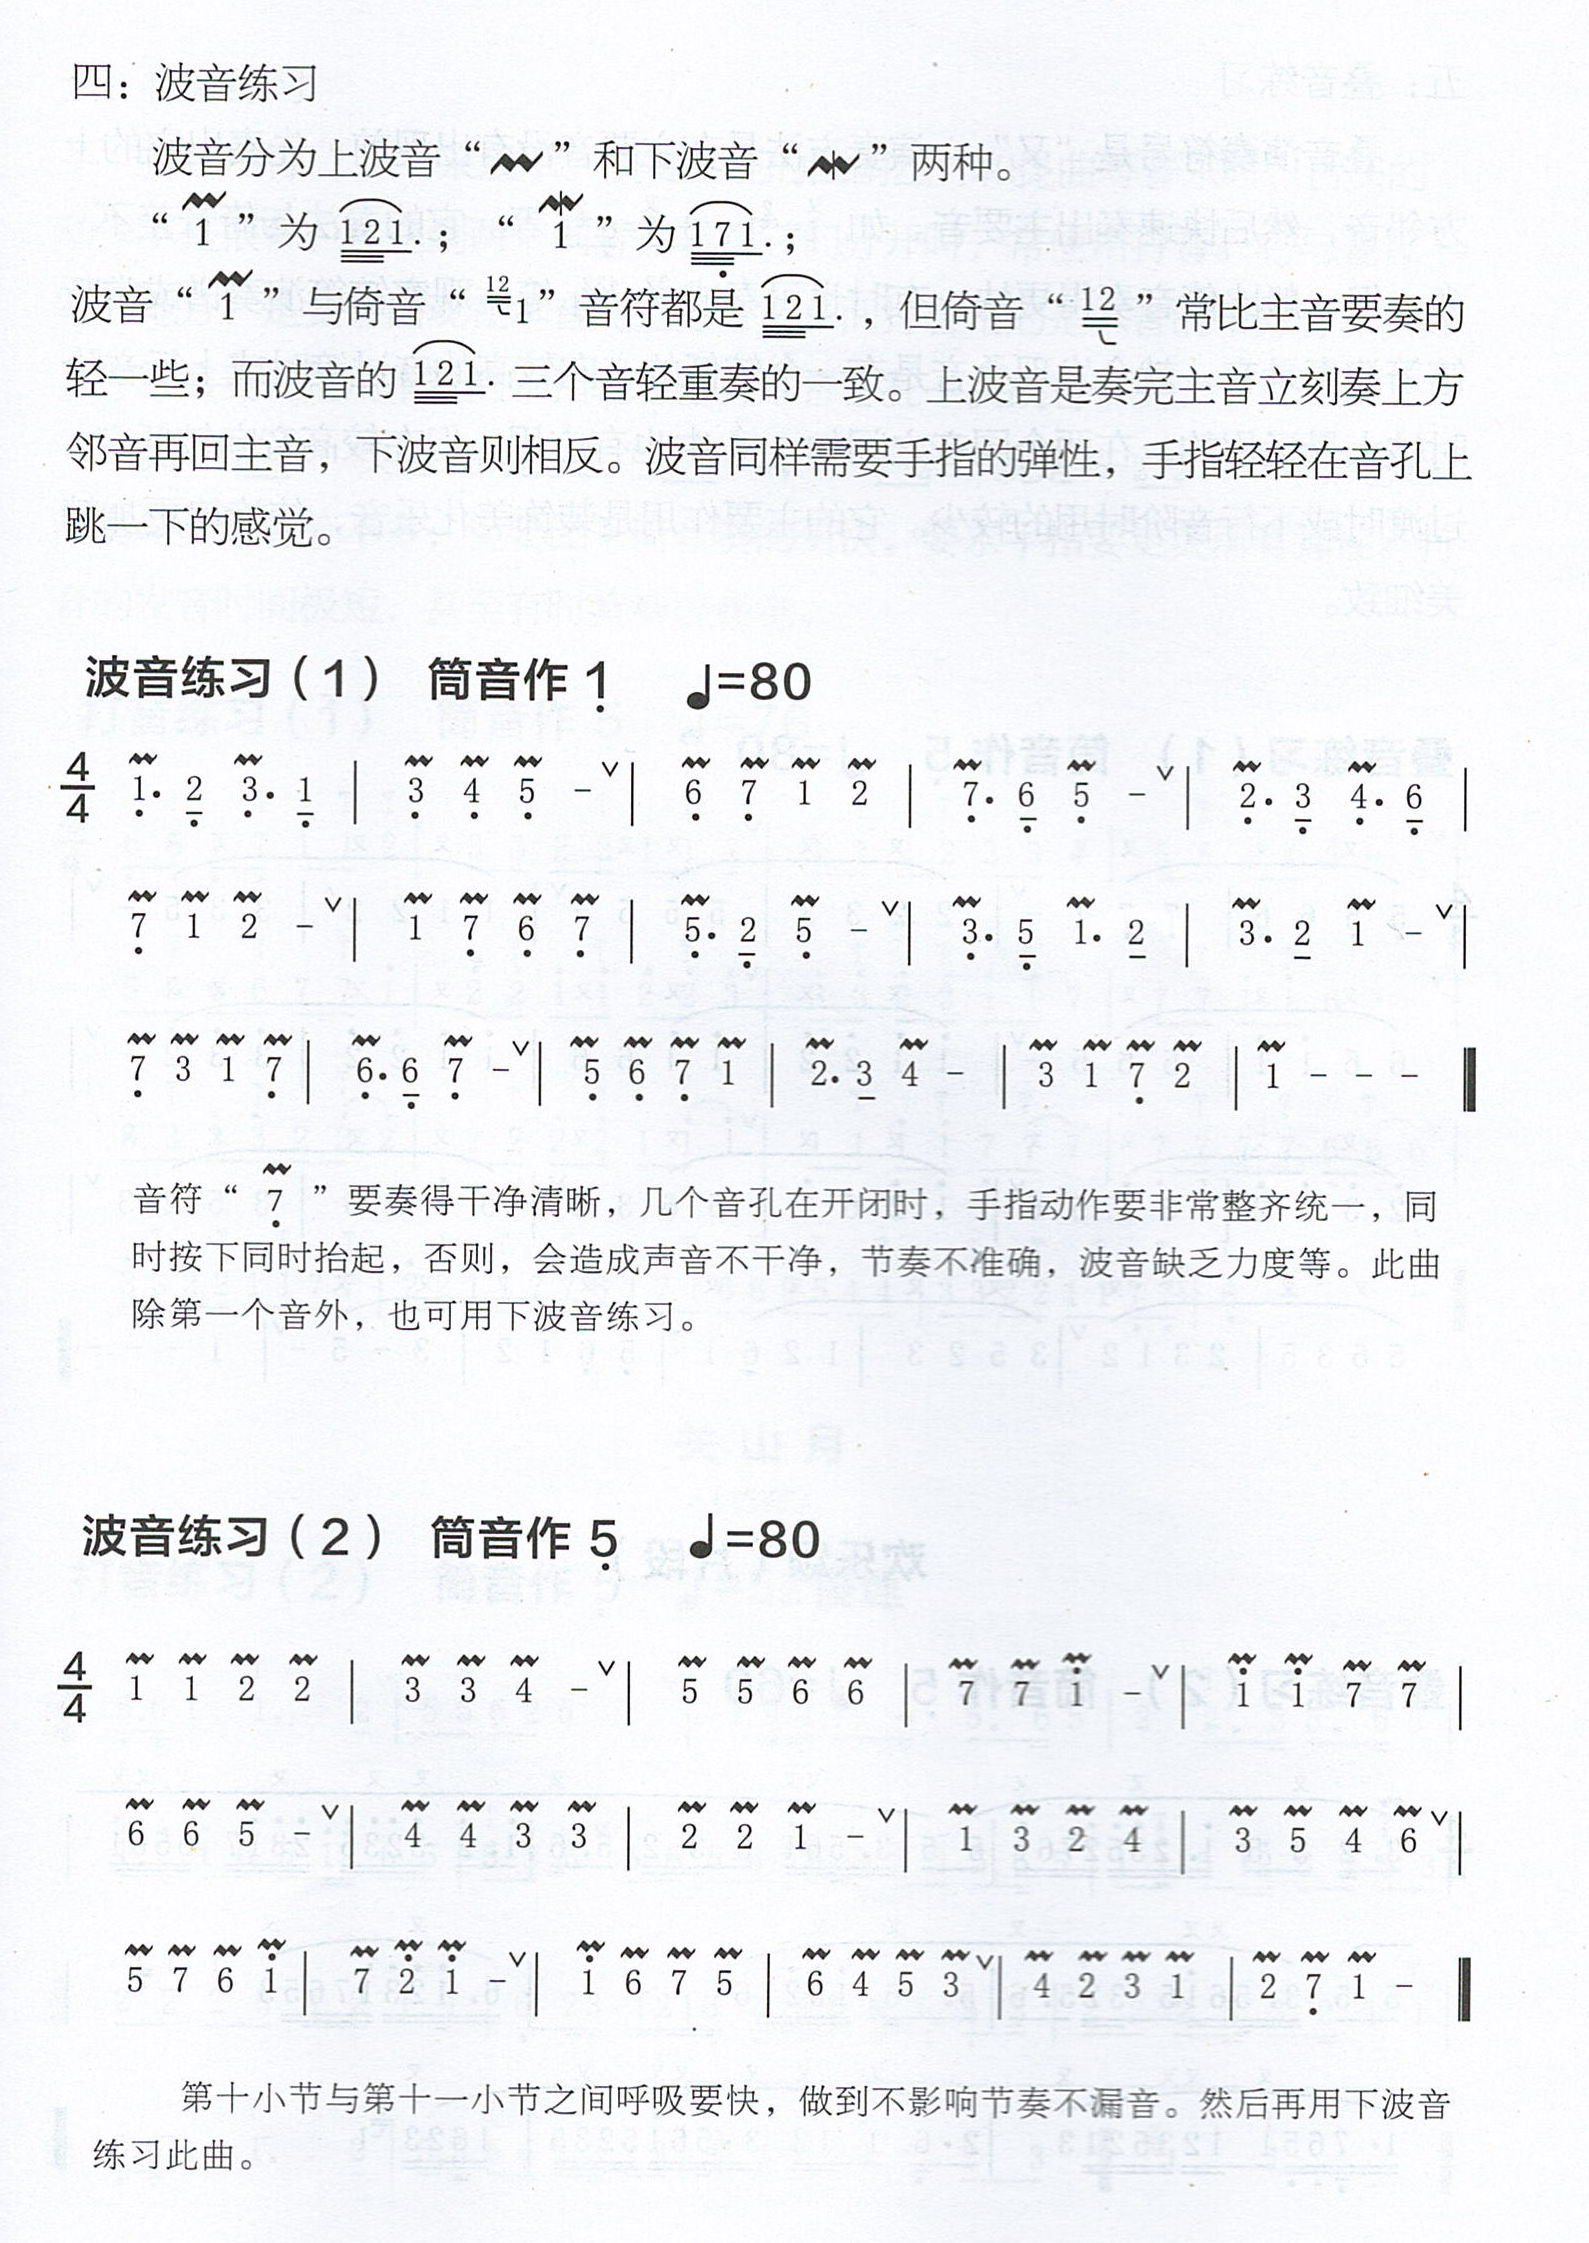
\includegraphics[height=\textheight]{dongxiao/Scan 10.jpeg}

\section{叠音练习(1全按作低音5,2全按作低音5 欢乐颂)}
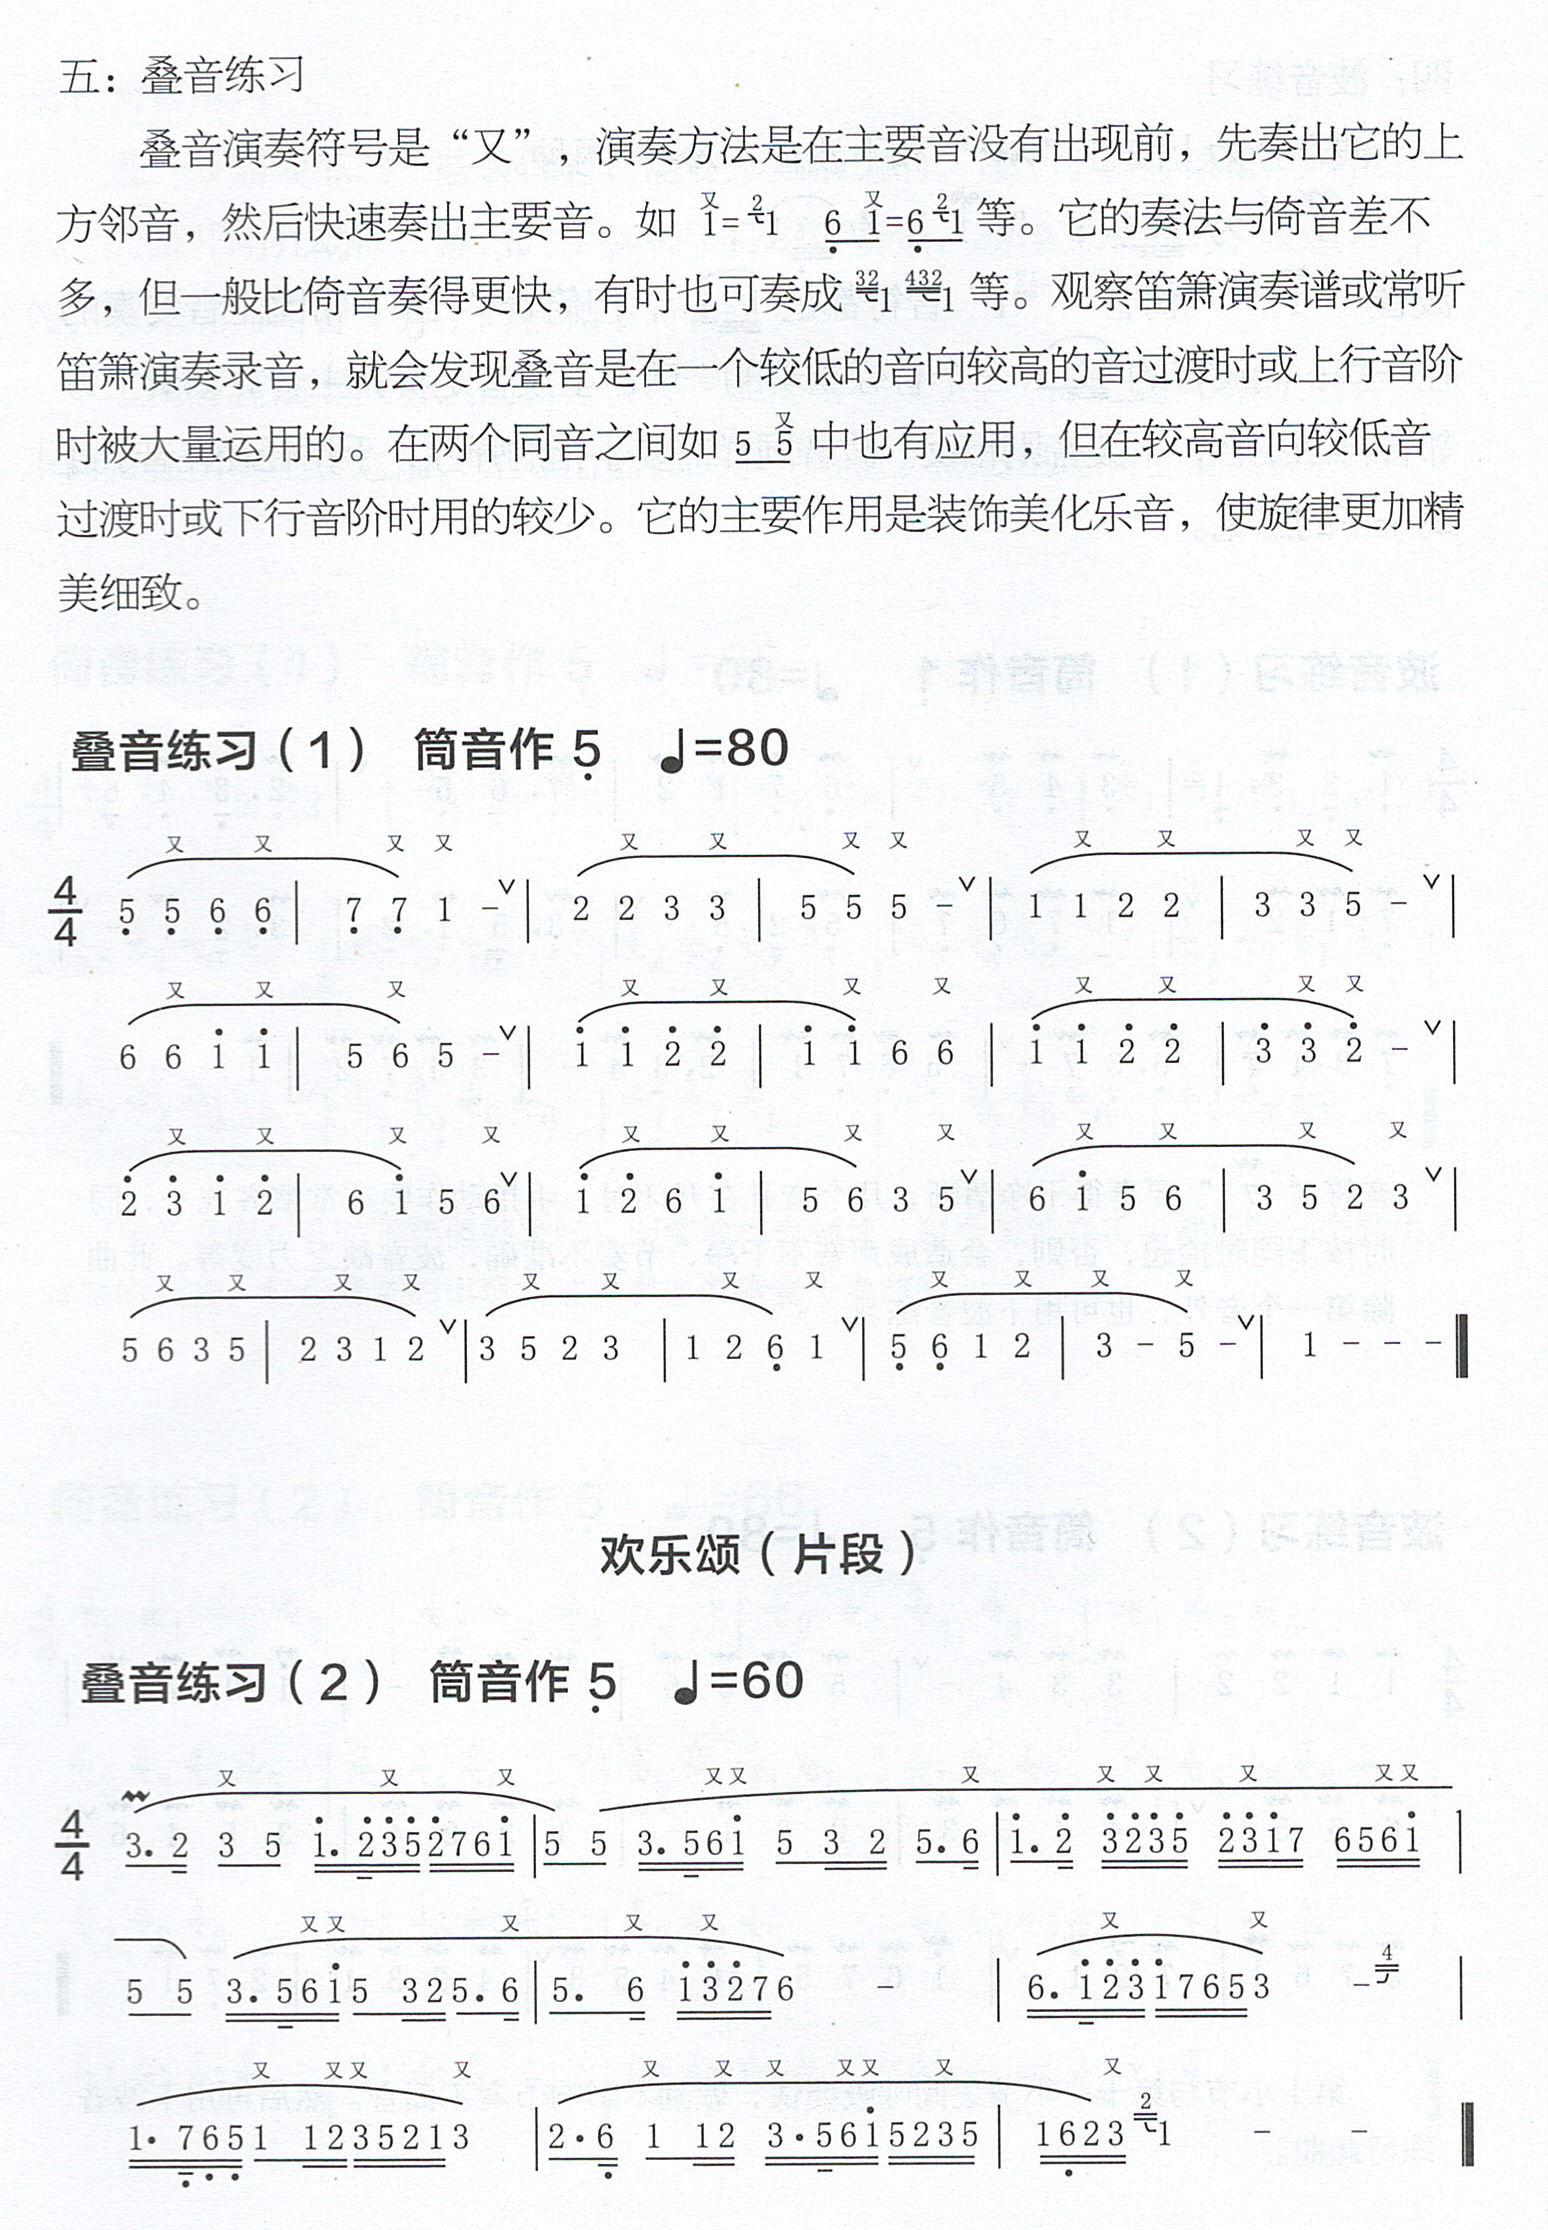
\includegraphics[height=\textheight]{dongxiao/Scan 11.jpeg}

\section{打音练习(1全按作低音5,2全按作低音5 关山月)}
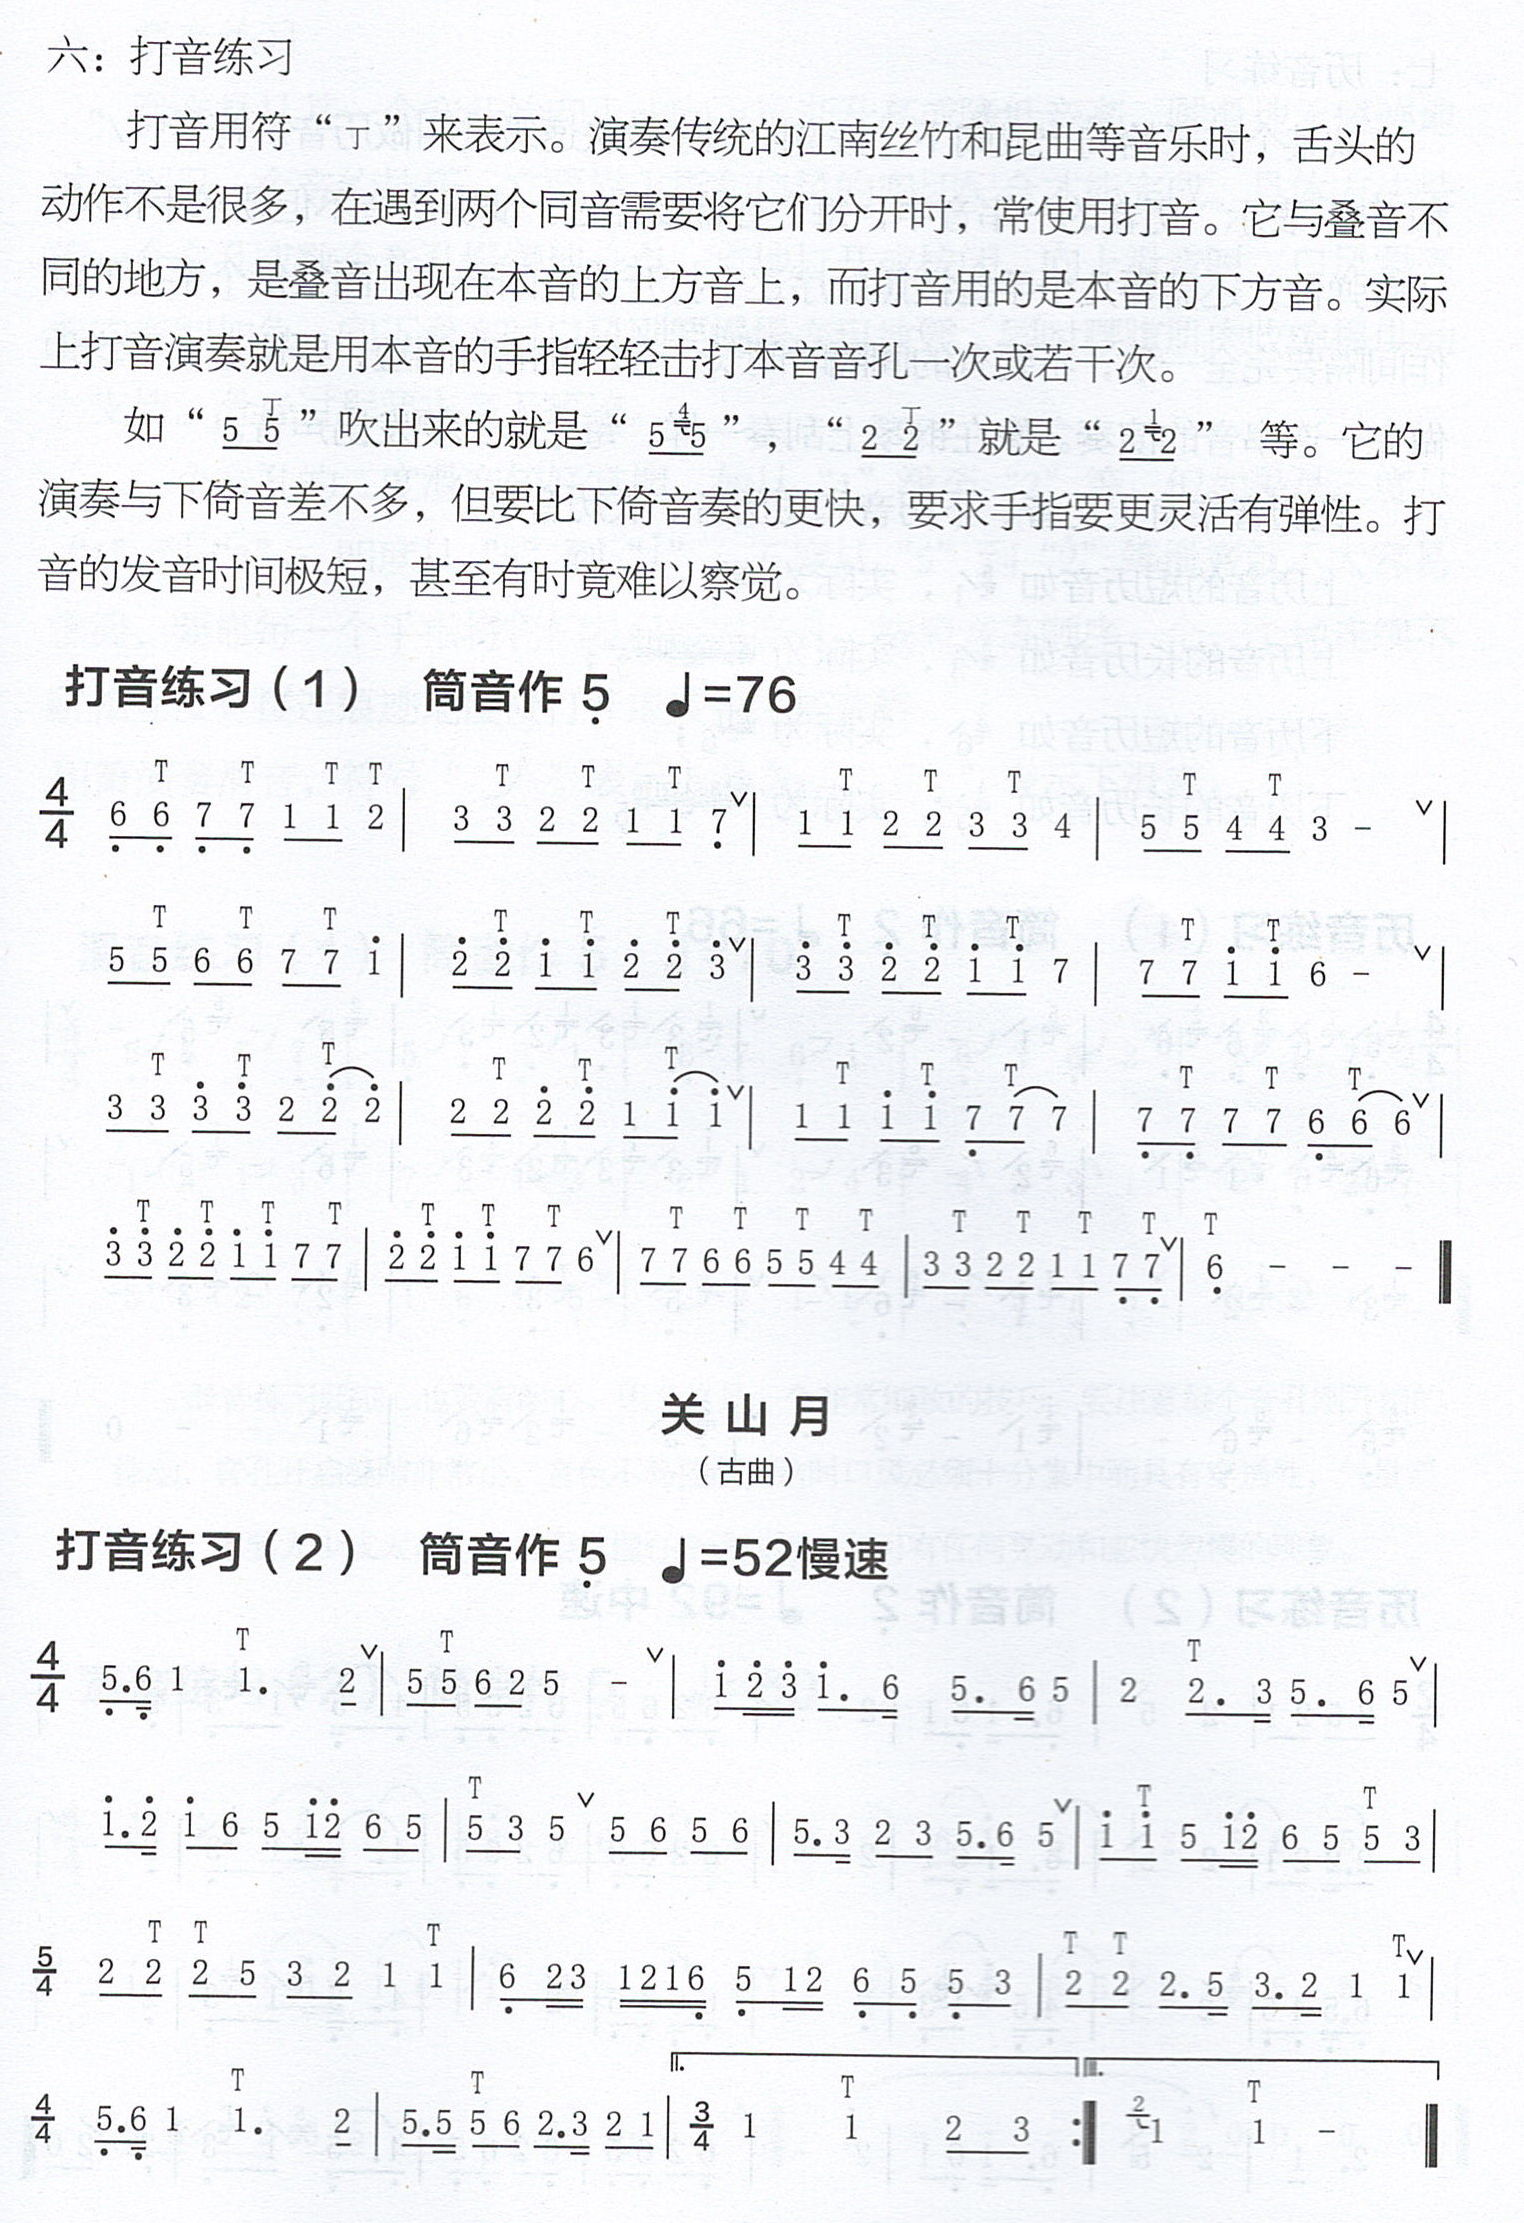
\includegraphics[height=\textheight]{dongxiao/Scan 12.jpeg}

\section{历音练习(1全按作低音2,2全按作低音2)}
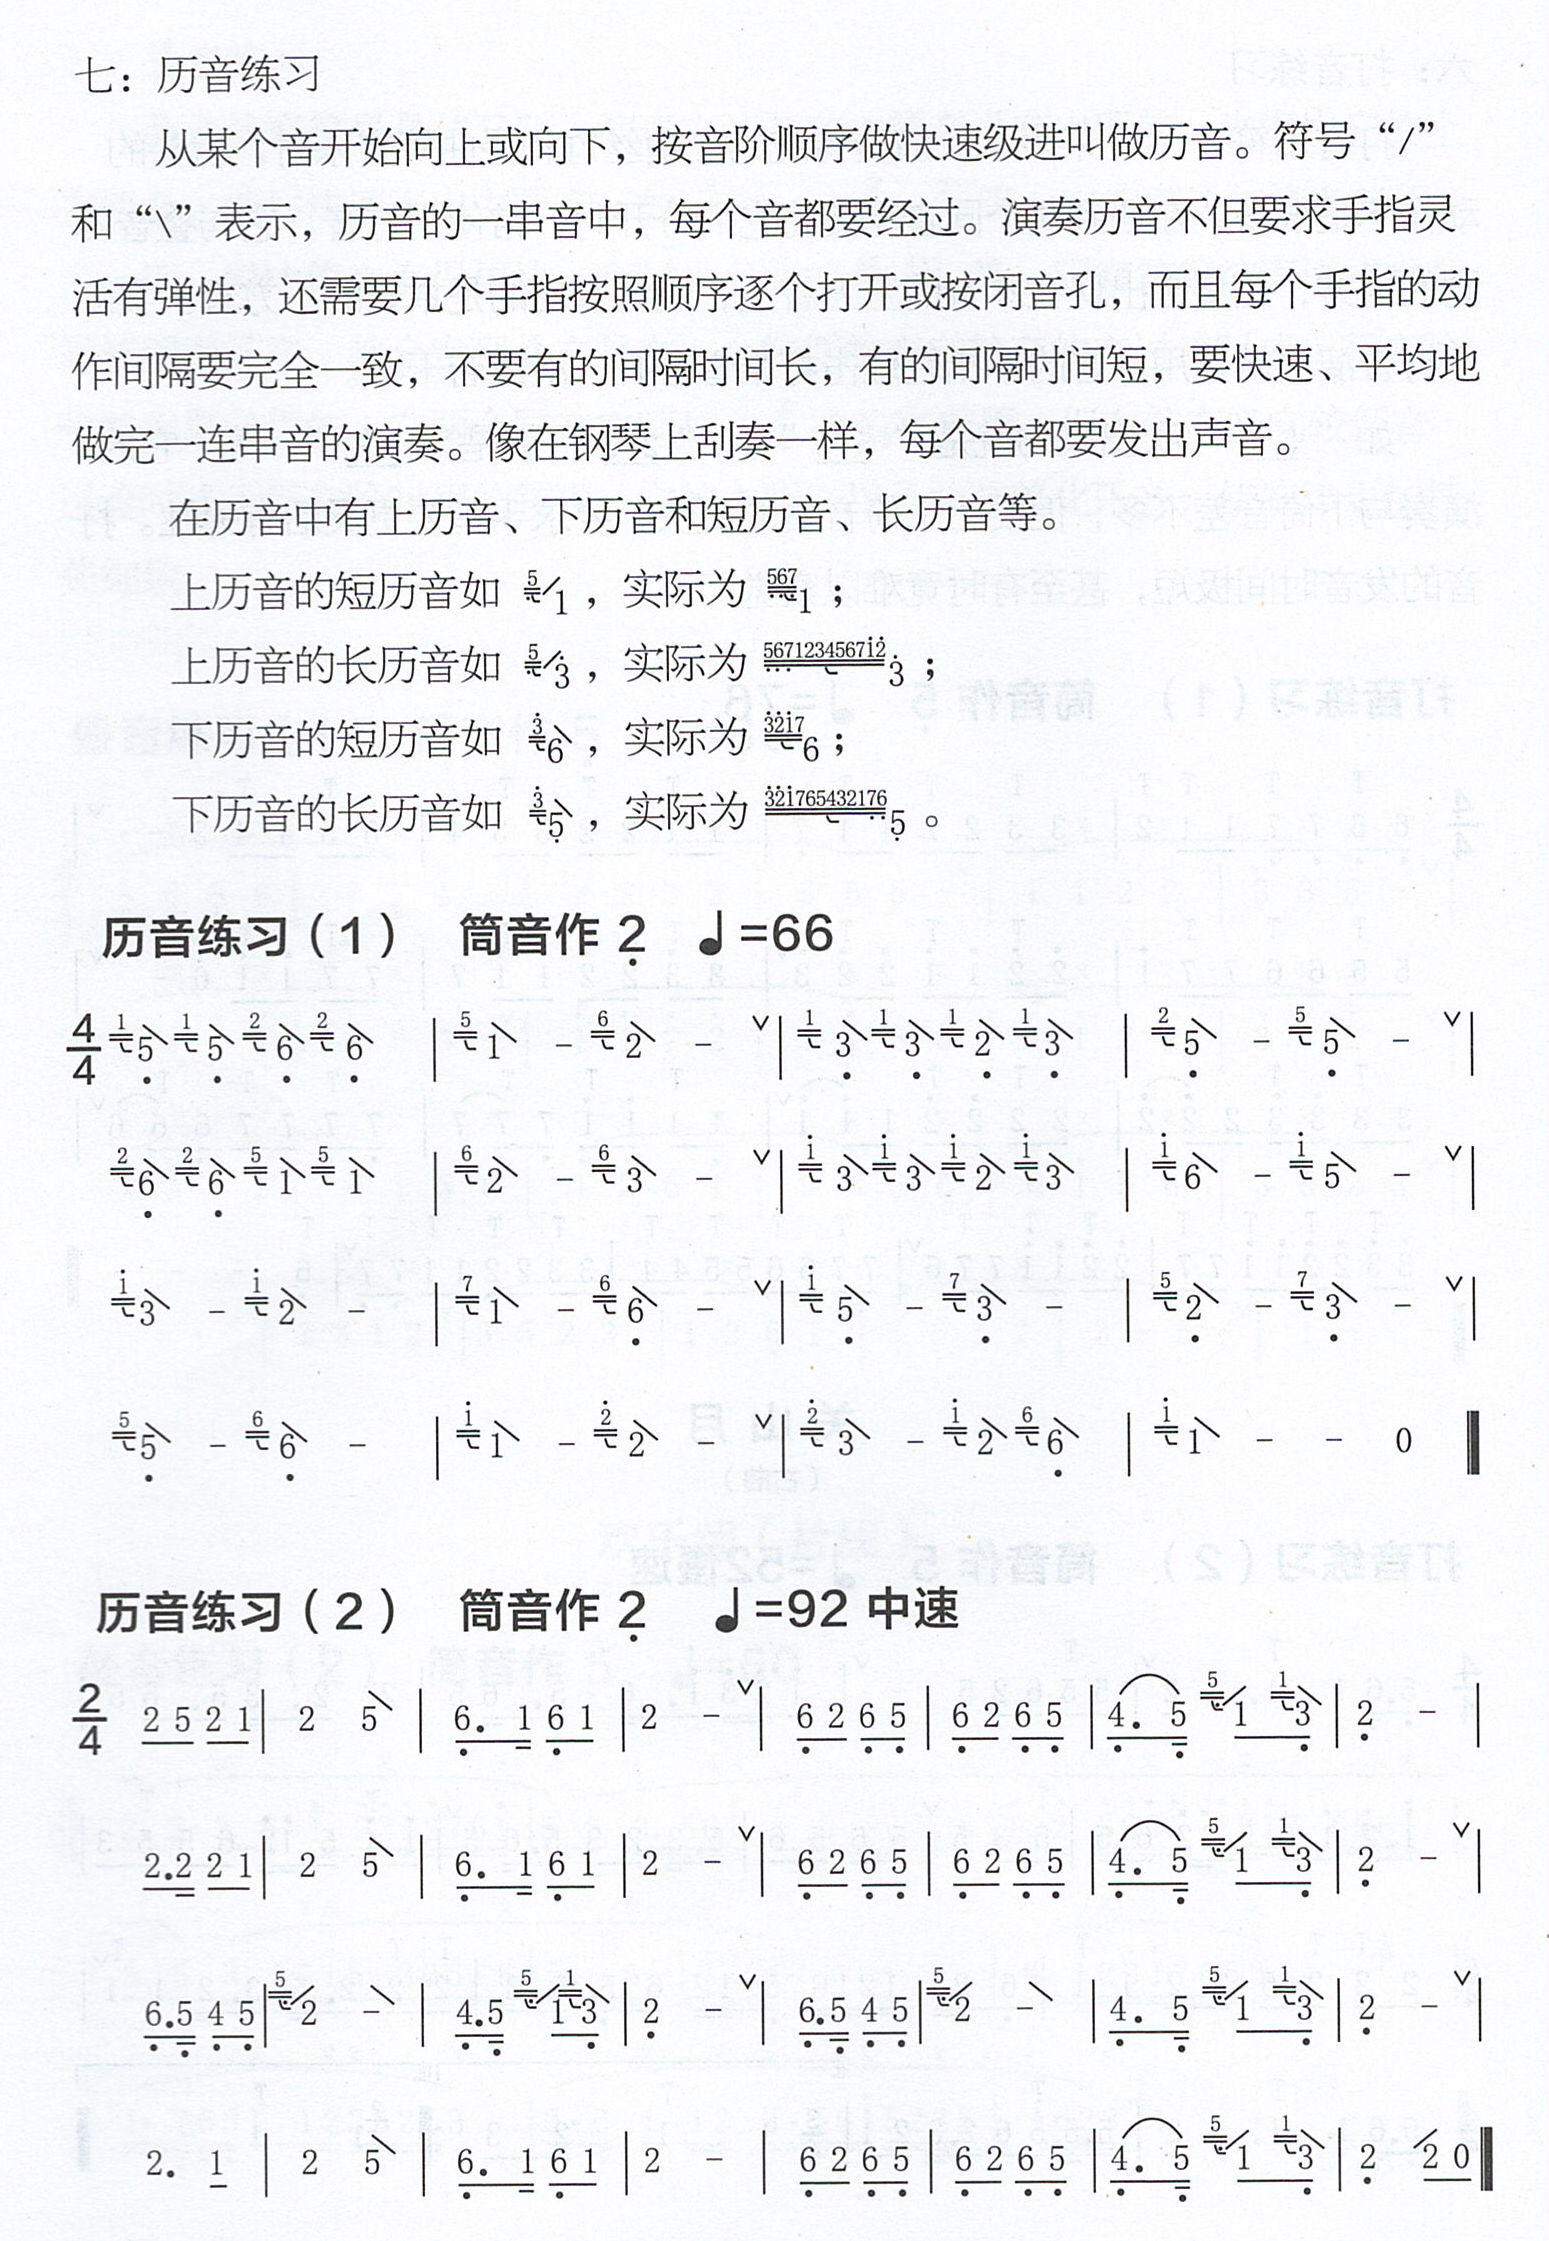
\includegraphics[height=\textheight]{dongxiao/Scan 13.jpeg}

\section{滑音练习(1全按作低音5,2全按作低音5)}
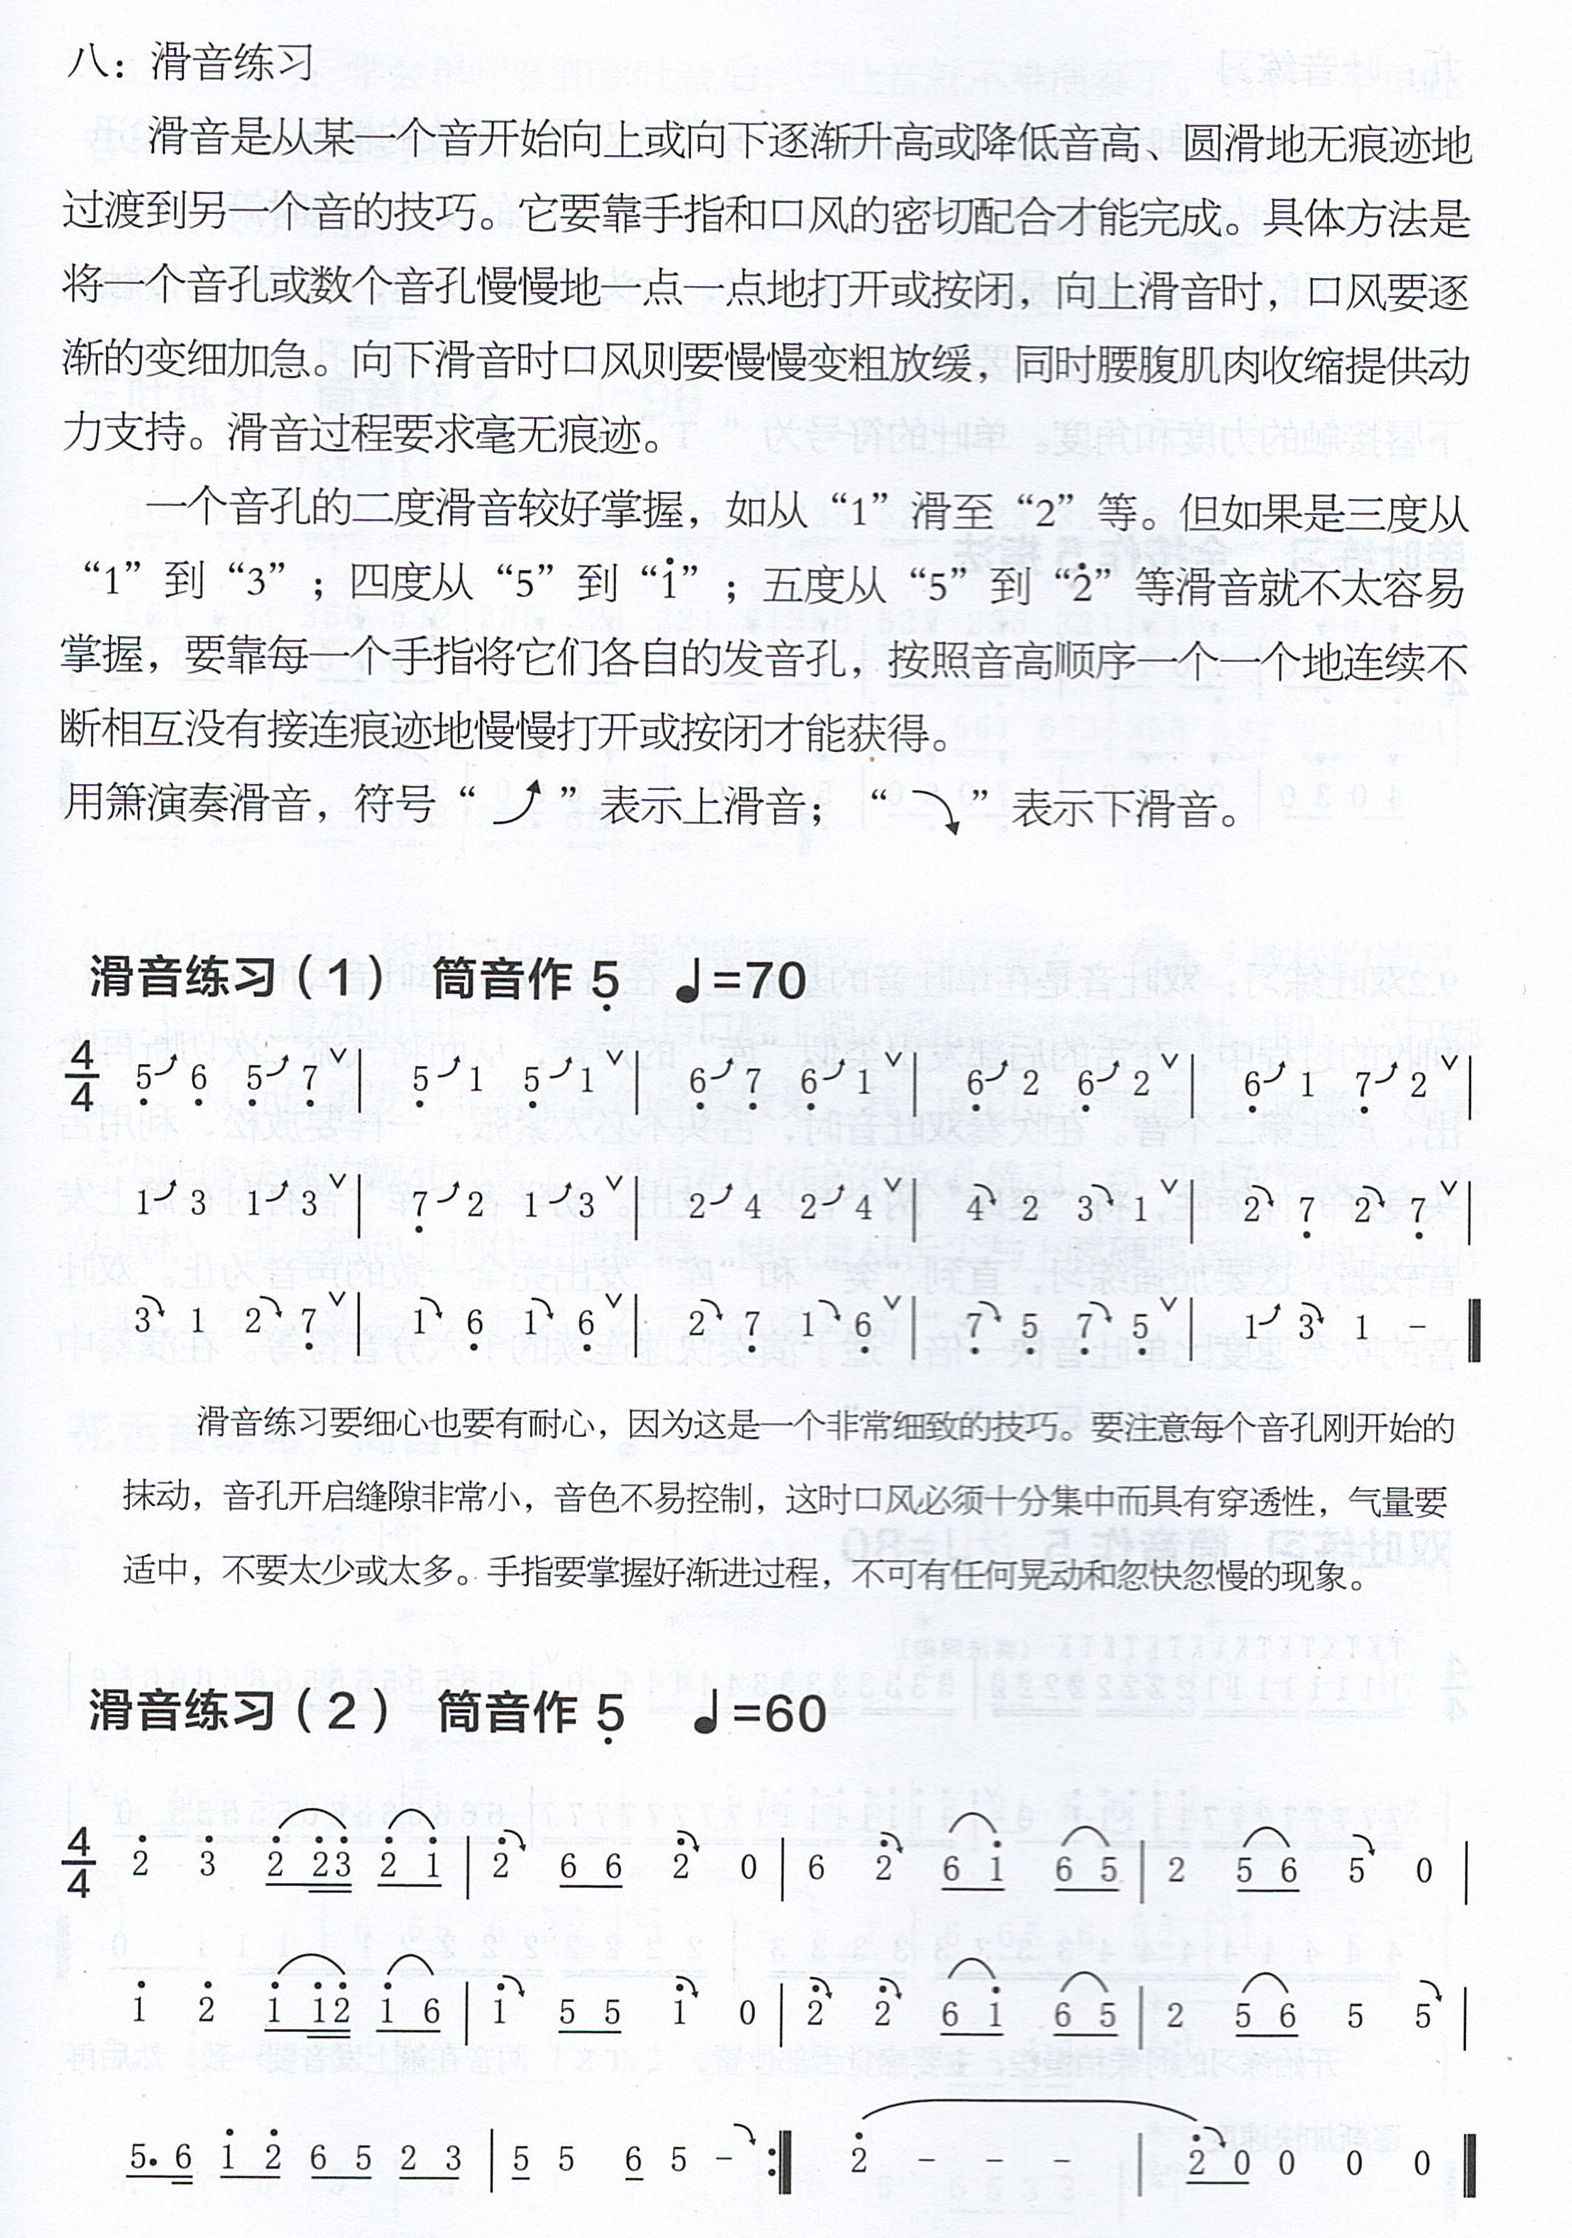
\includegraphics[height=\textheight]{dongxiao/Scan 14.jpeg}

\section{吐音练习(1单吐音 全按作低音5,2双吐音 全按作低音5)}
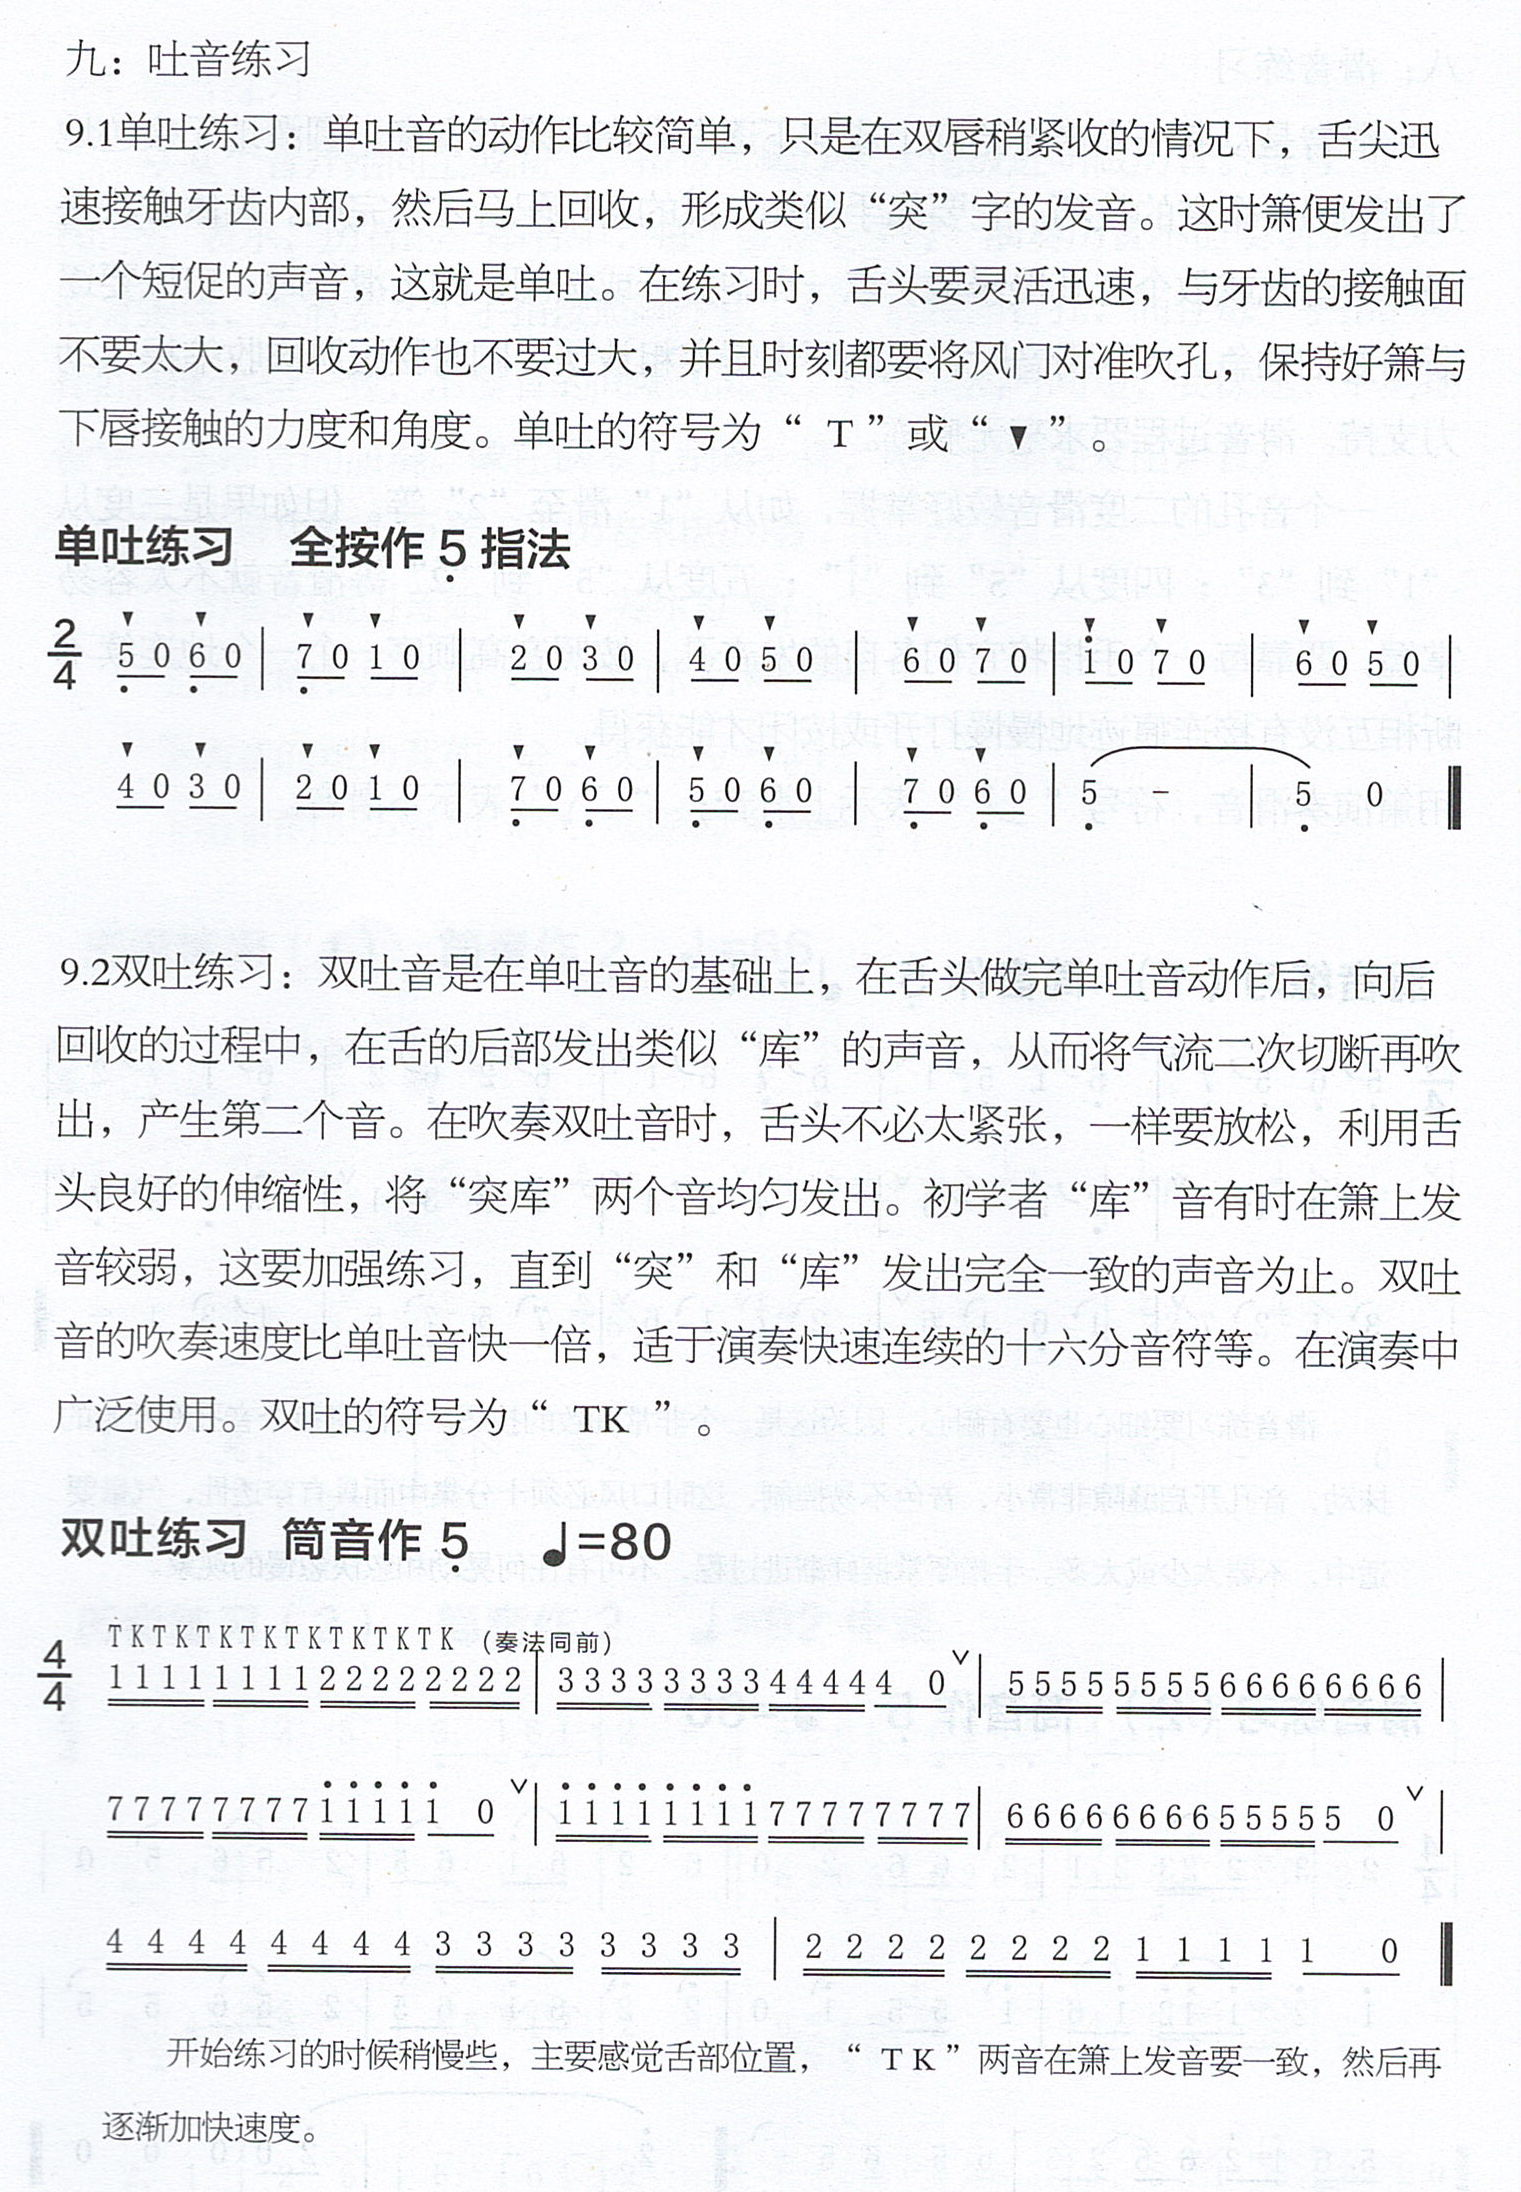
\includegraphics[height=\textheight]{dongxiao/Scan 15.jpeg}

\section{吐音练习(3三吐音 全按作低音2)}
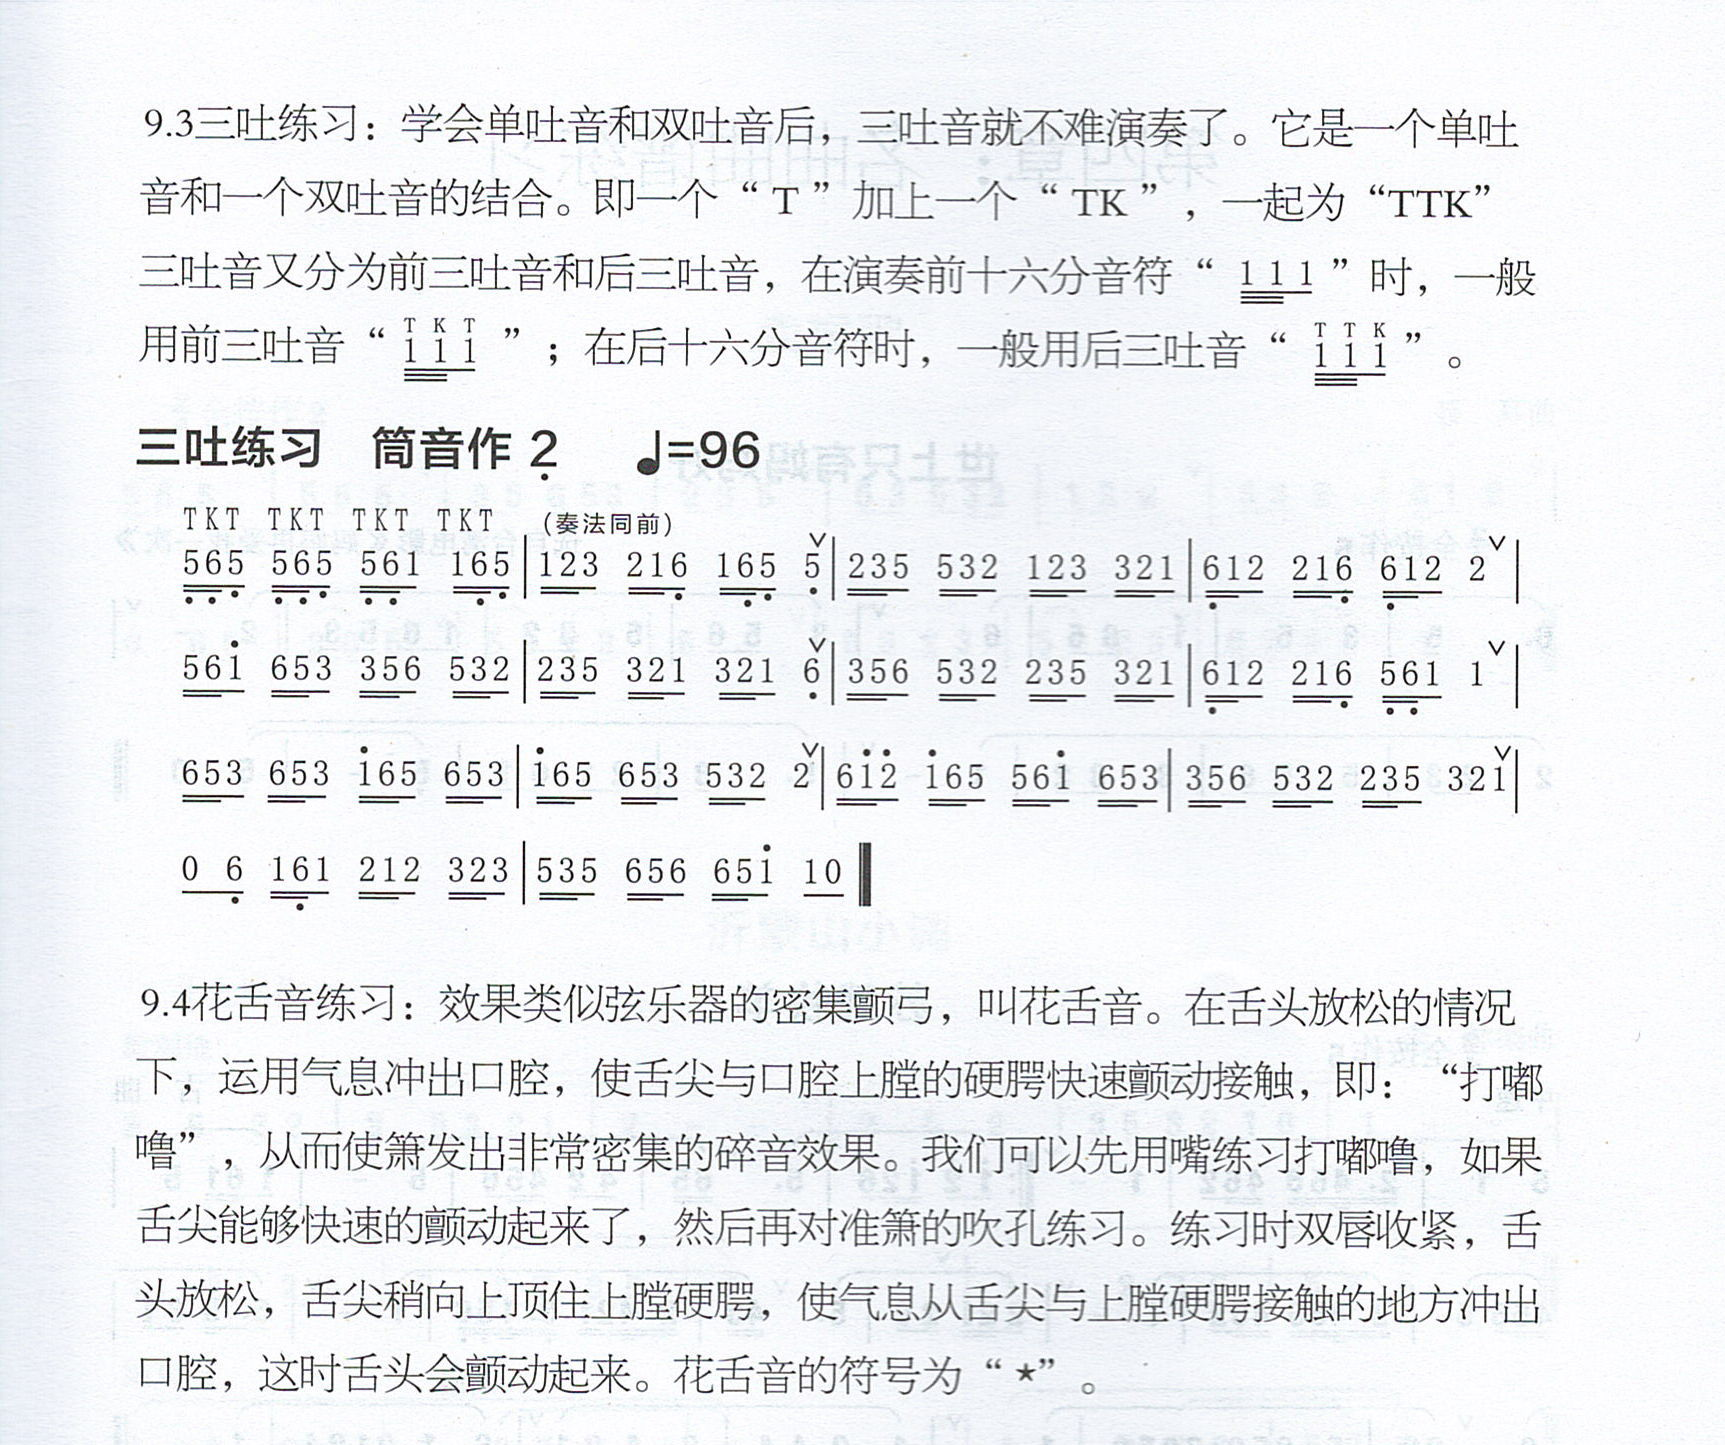
\includegraphics[width=\textwidth]{dongxiao/Scan 16-1.jpeg}
\section{花舌音练习(全按作低音5)}
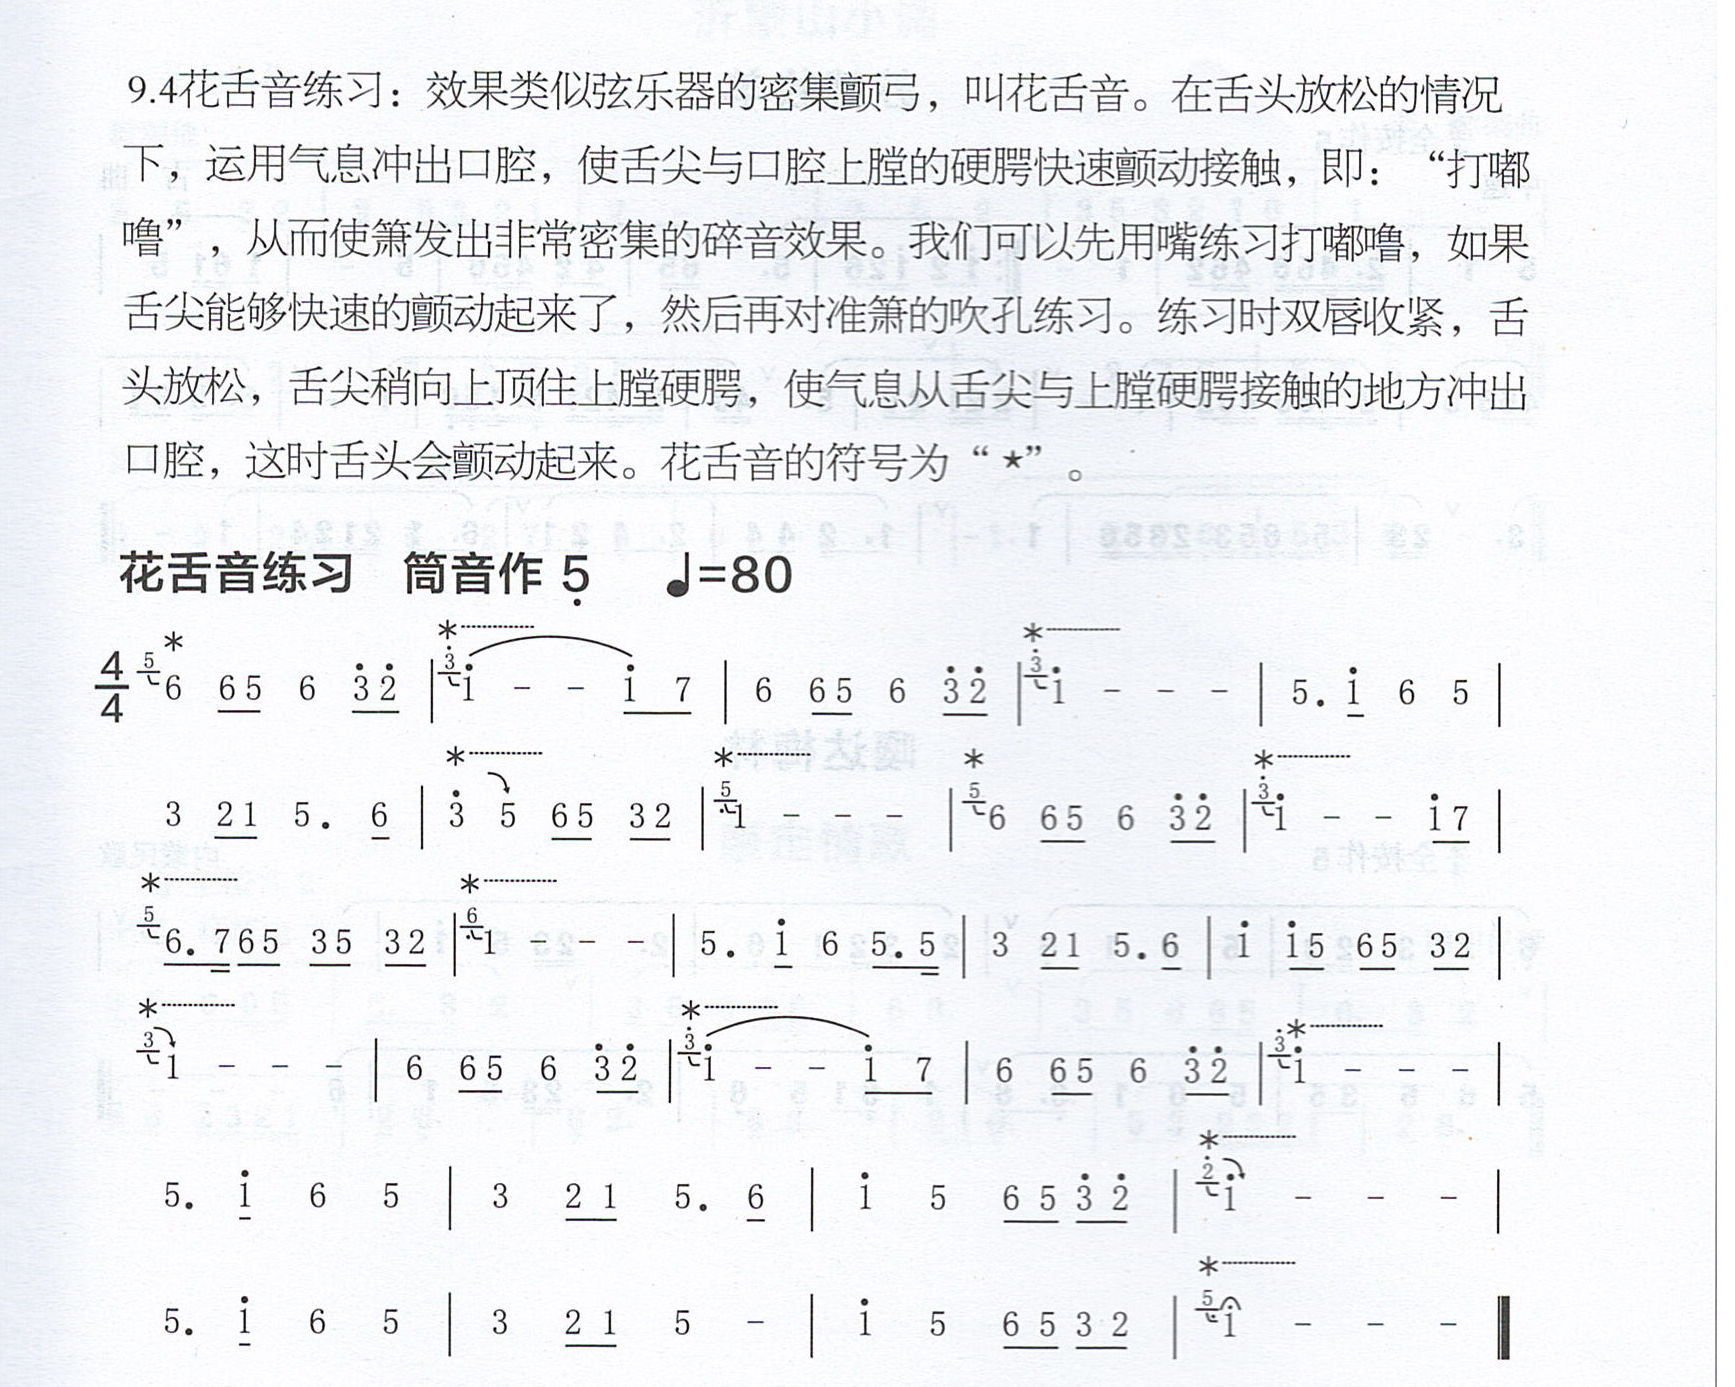
\includegraphics[width=\textwidth]{dongxiao/Scan 16-2.jpeg}

\chapter{曲谱练习}
\section{世上只有妈妈好}
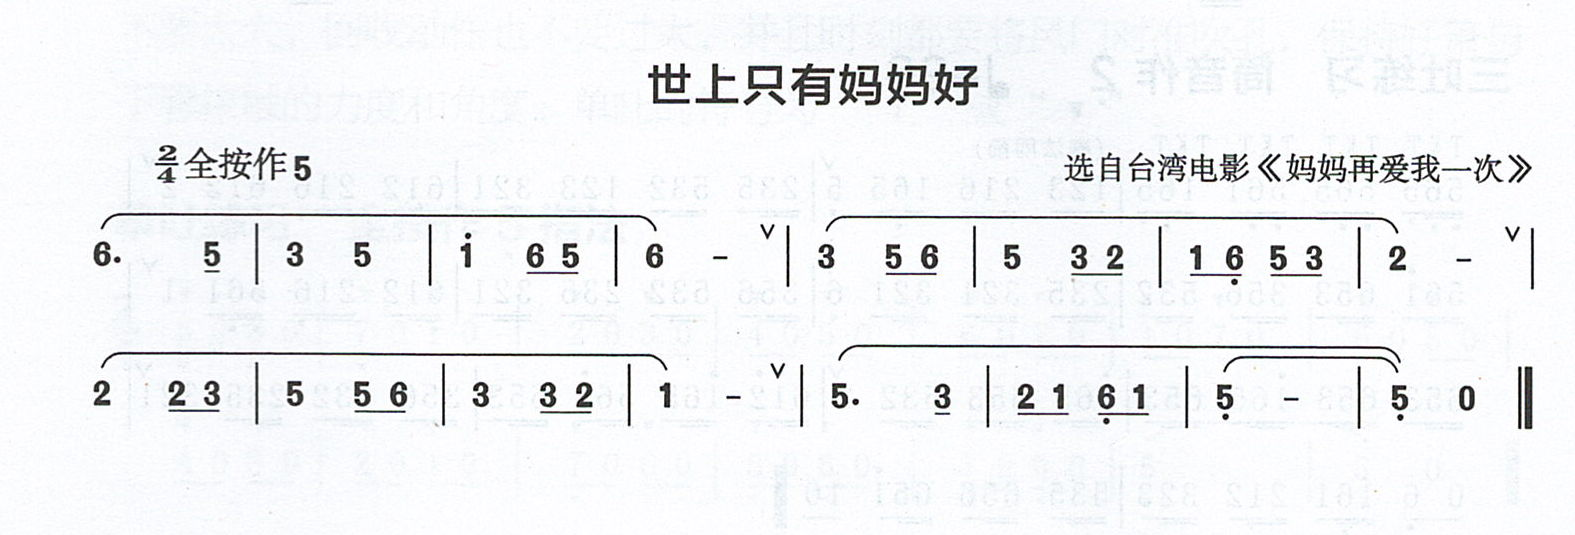
\includegraphics[width=\textwidth]{dongxiao/Scan 17-1.jpeg}
\section{苏武牧羊}
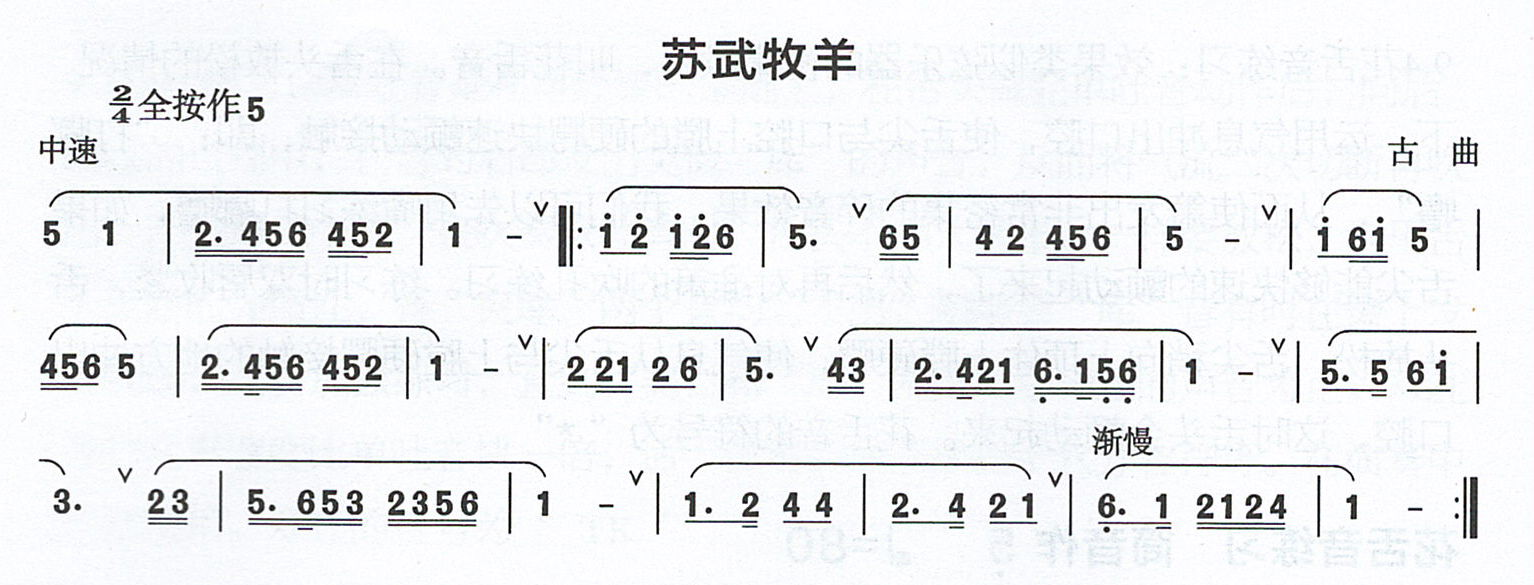
\includegraphics[width=\textwidth]{dongxiao/Scan 17-2.jpeg}
\section{嘎达梅林}
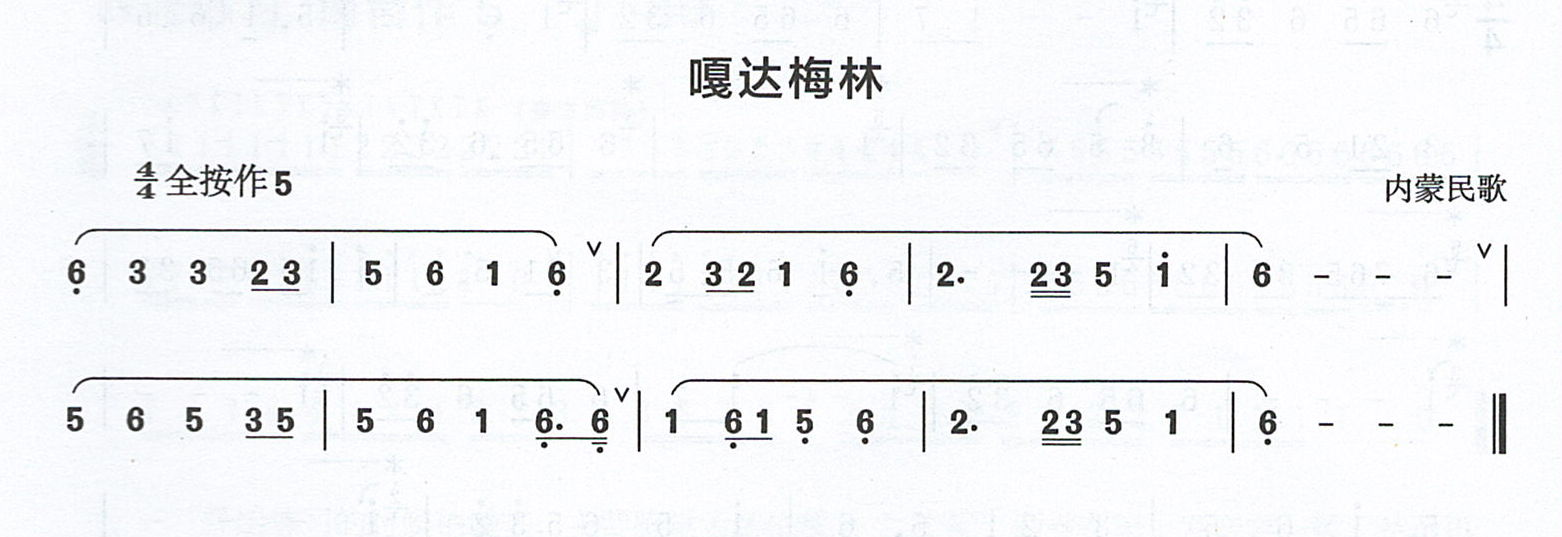
\includegraphics[width=\textwidth]{dongxiao/Scan 17-3.jpeg}

\section{卖报歌}
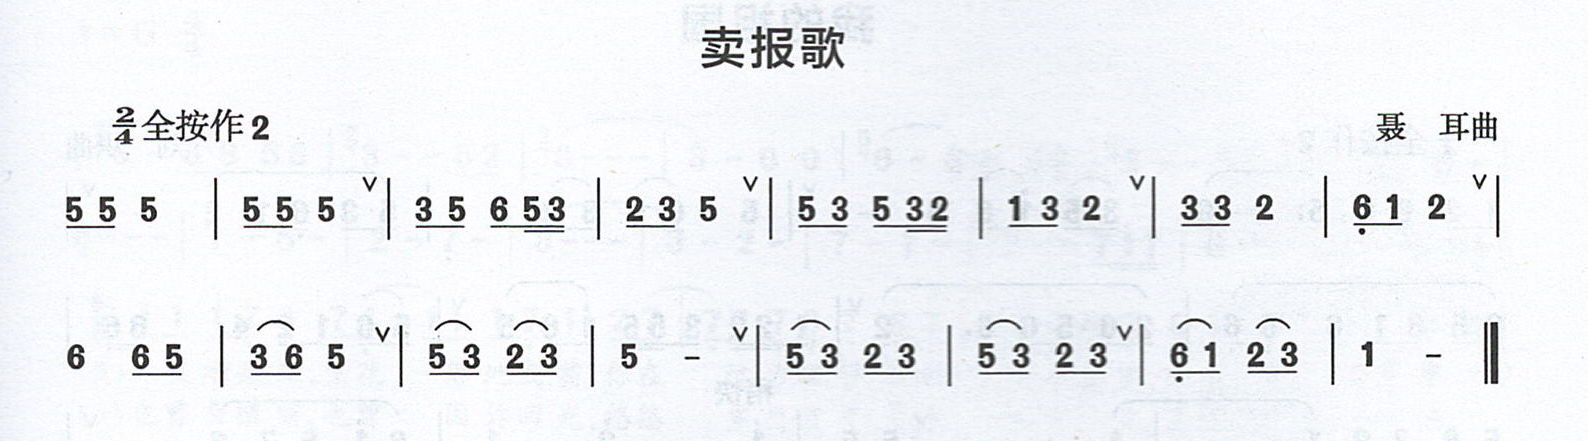
\includegraphics[width=\textwidth]{dongxiao/Scan 18-1.jpeg}
\section{沂蒙山小调}
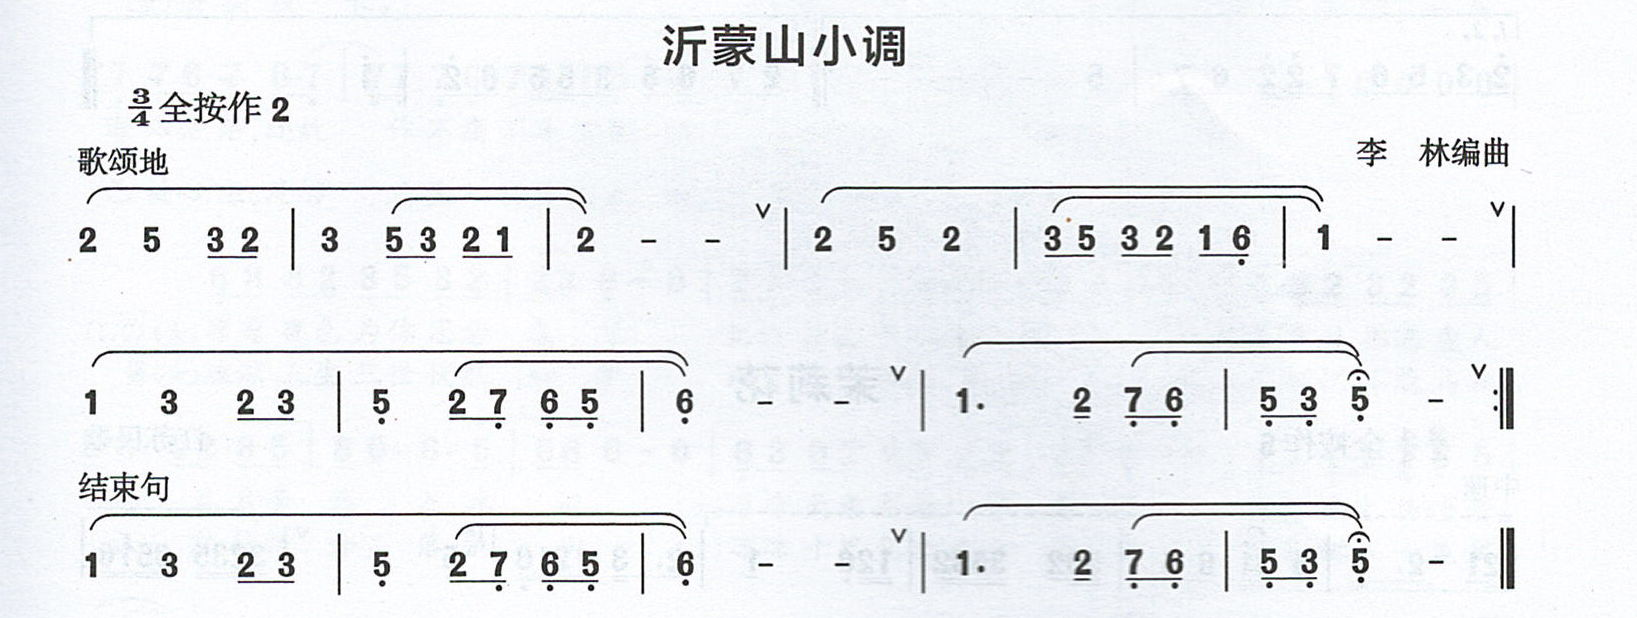
\includegraphics[width=\textwidth]{dongxiao/Scan 18-2.jpeg}
\section{康定情歌}
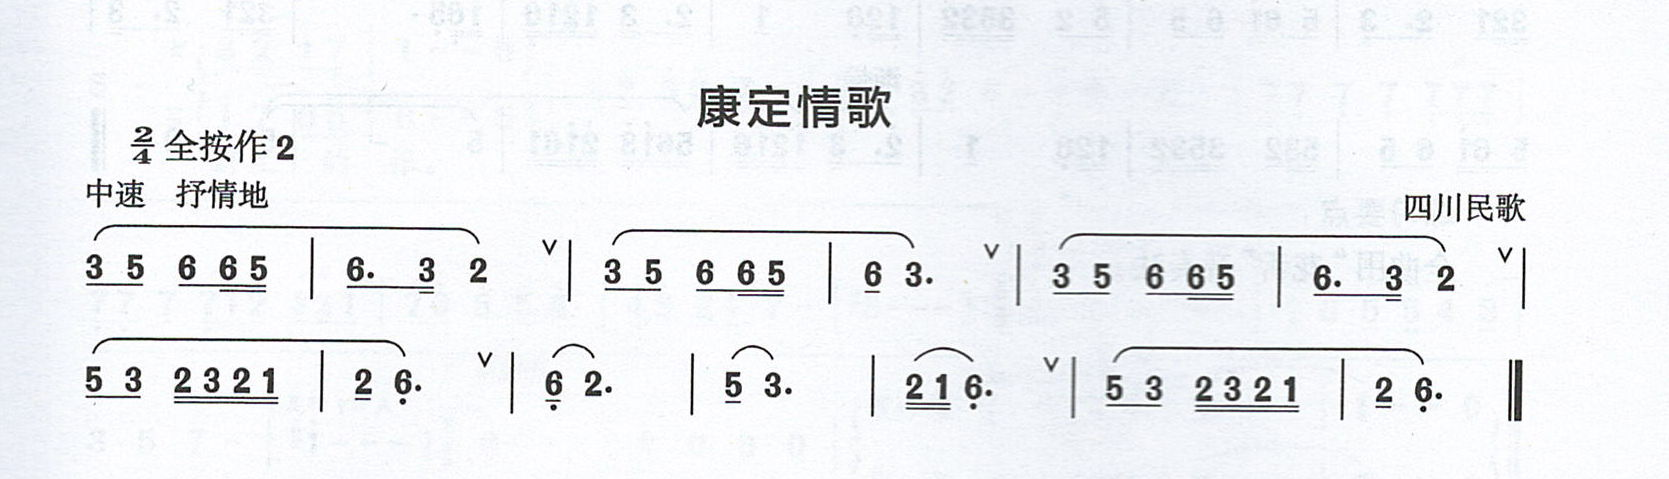
\includegraphics[width=\textwidth]{dongxiao/Scan 18-3.jpeg}

\section{我的祖国}
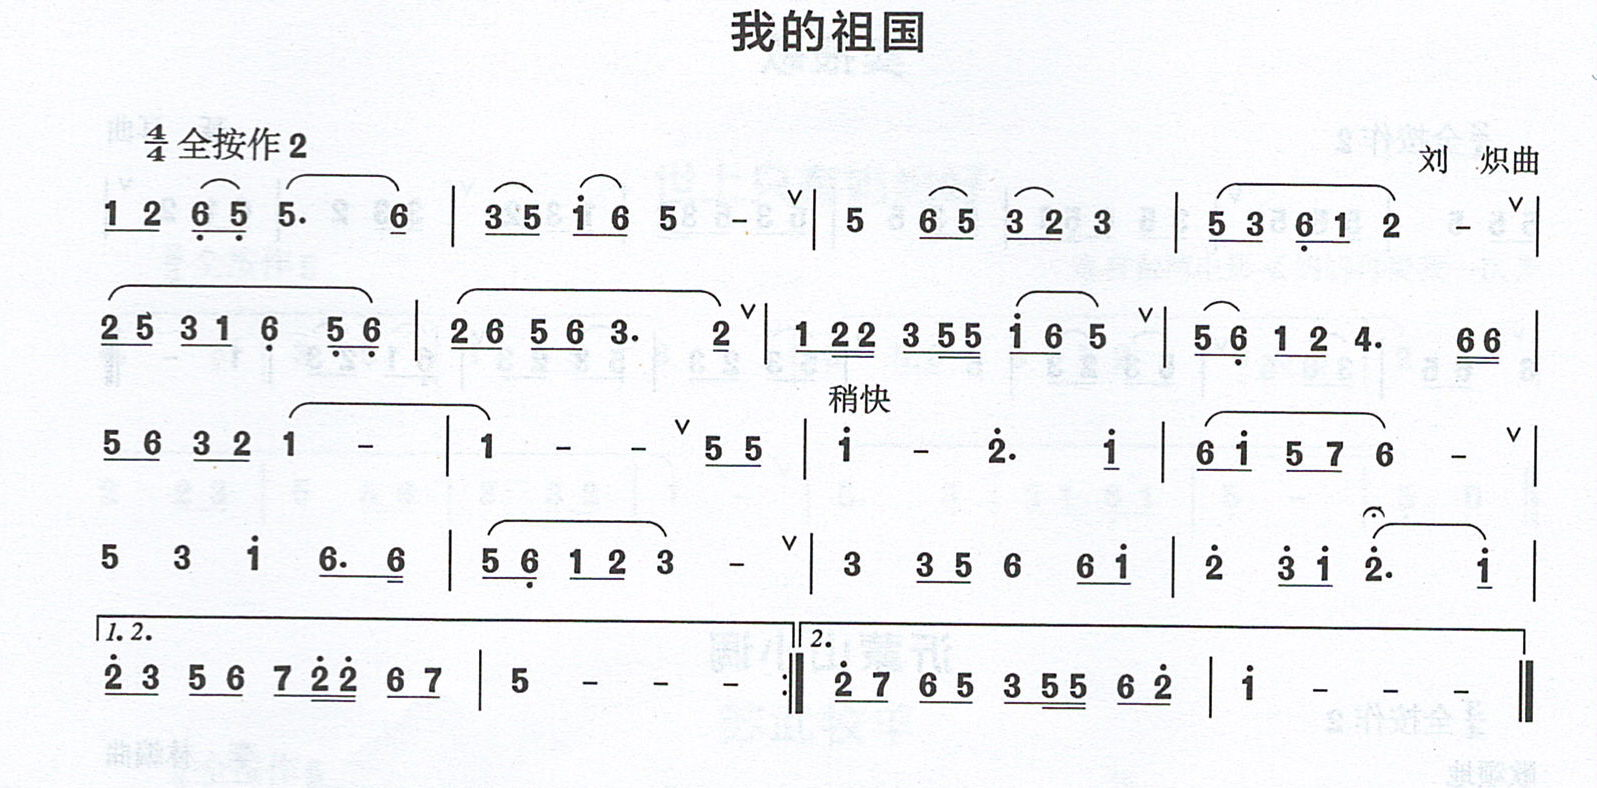
\includegraphics[width=\textwidth]{dongxiao/Scan 19-1.jpeg}
\section{茉莉花}
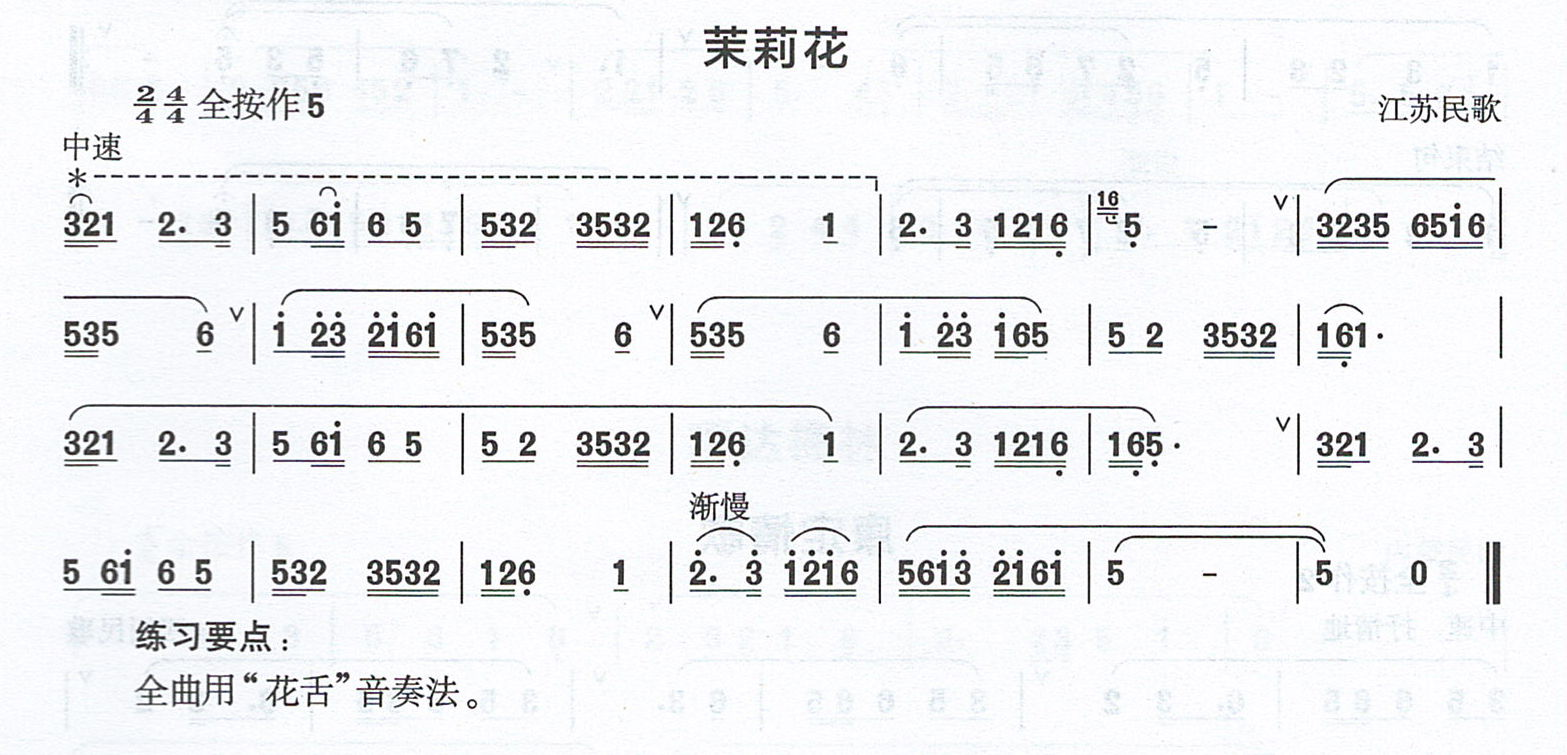
\includegraphics[width=\textwidth]{dongxiao/Scan 19-2.jpeg}

\section{小草}
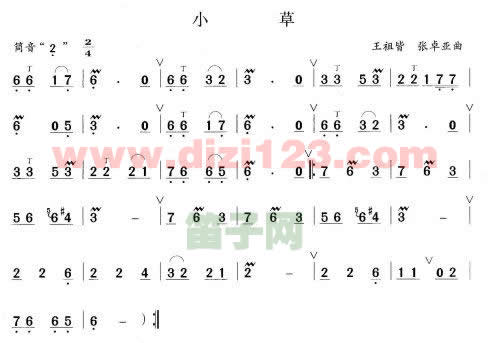
\includegraphics[width=\textwidth]{dongxiao/小草.jpg}
\section{思归乐}
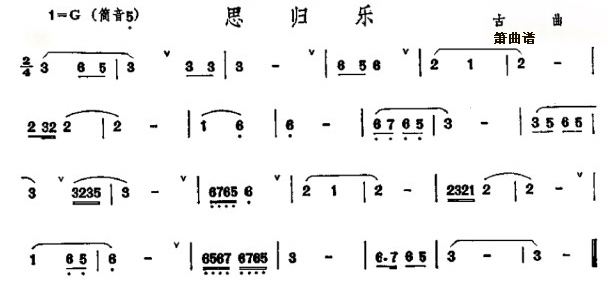
\includegraphics[width=\textwidth]{dongxiao/思归乐.jpg}
\section{一样的人}
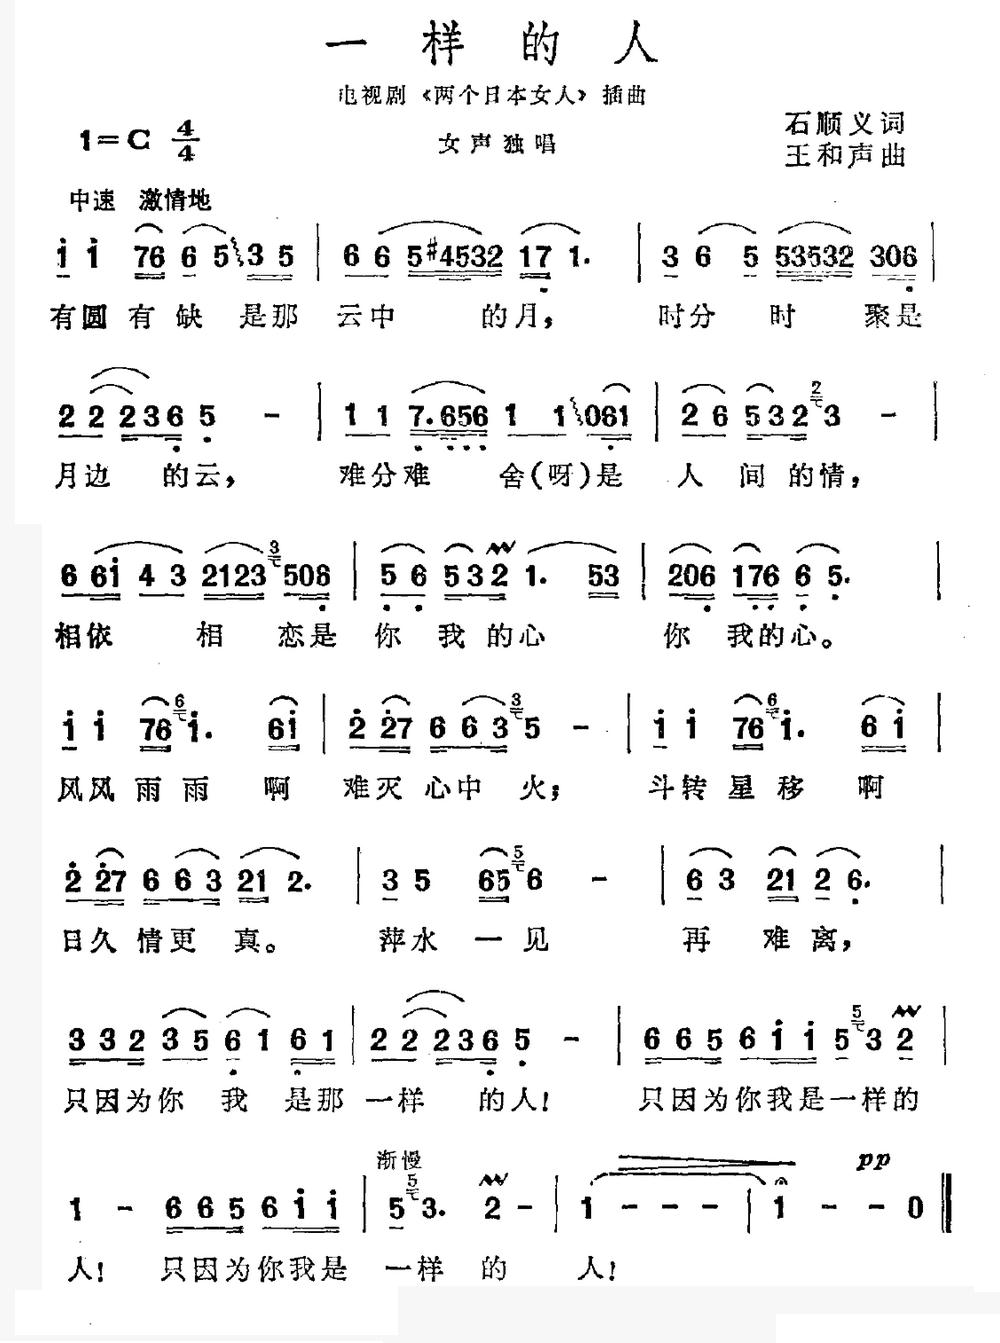
\includegraphics[height=\textheight]{dongxiao/日本-一样的人.jpg}
\section{八木调}
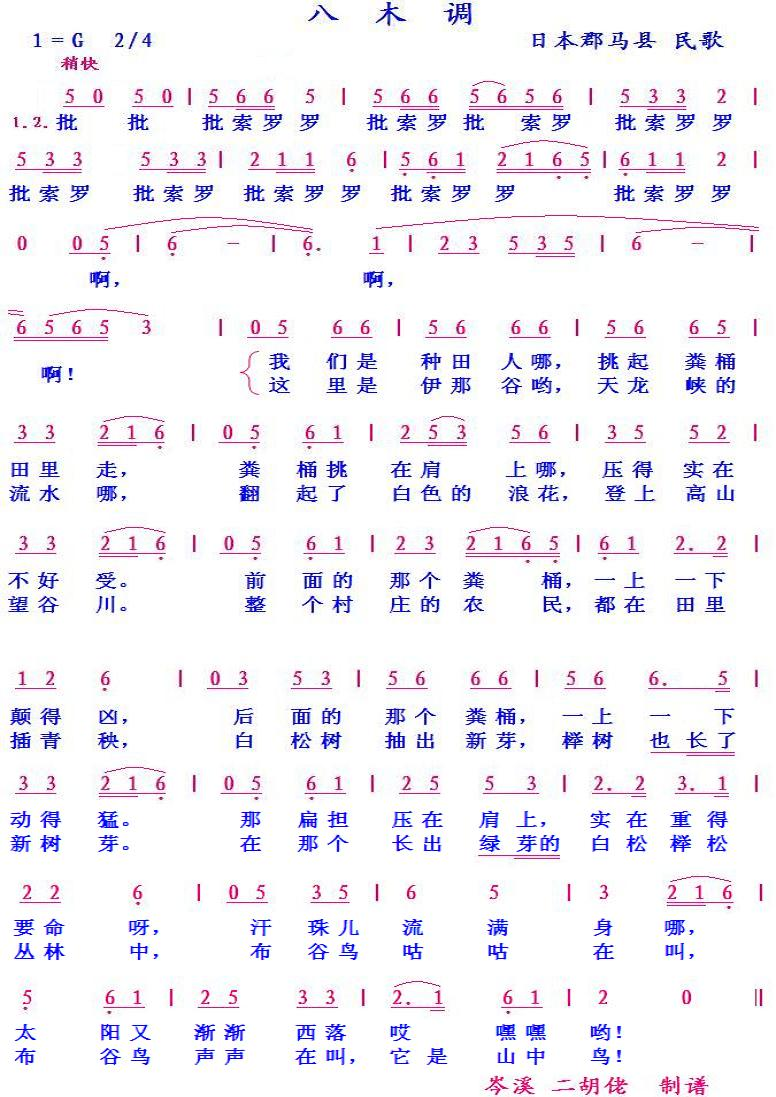
\includegraphics[height=\textheight]{dongxiao/日本-八木调.jpg}
\section{去野游}
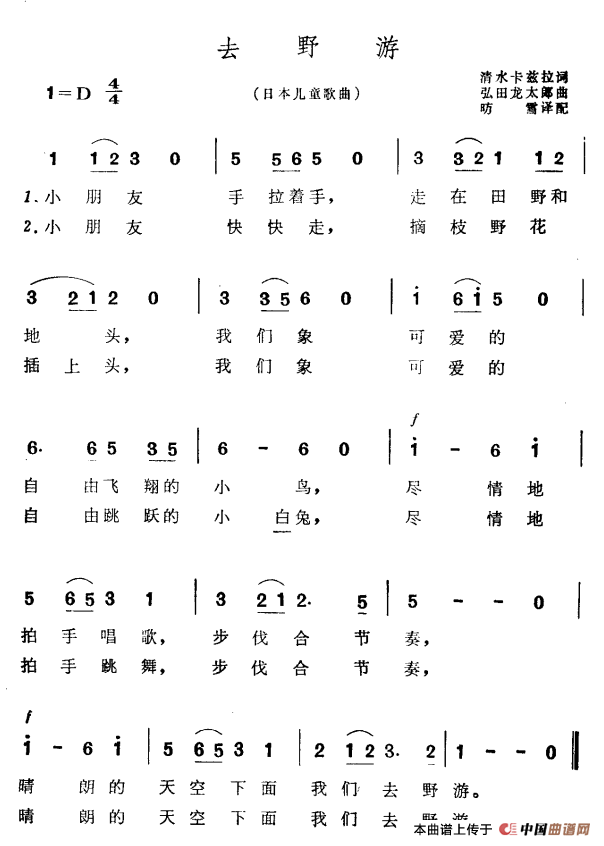
\includegraphics[height=\textheight]{dongxiao/日本-去野游.png}

\section{小路}
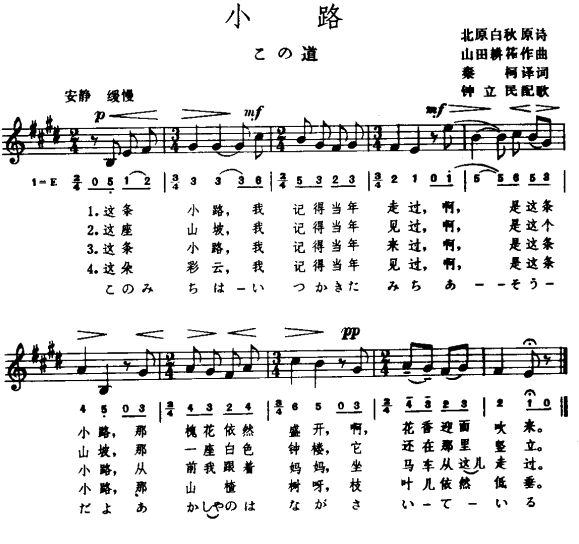
\includegraphics[width=\textwidth]{dongxiao/日本-小路.png}

\section{故乡}
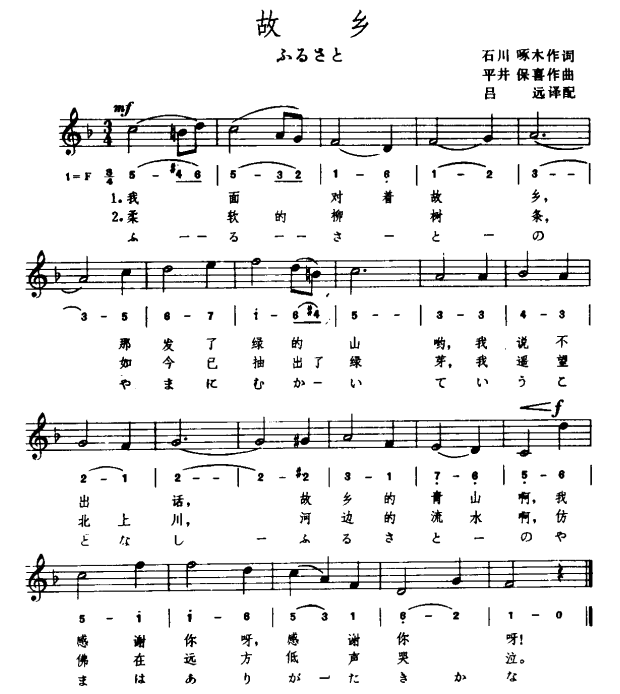
\includegraphics[width=\textwidth]{dongxiao/日本-故乡.png}

\section{春之歌}
    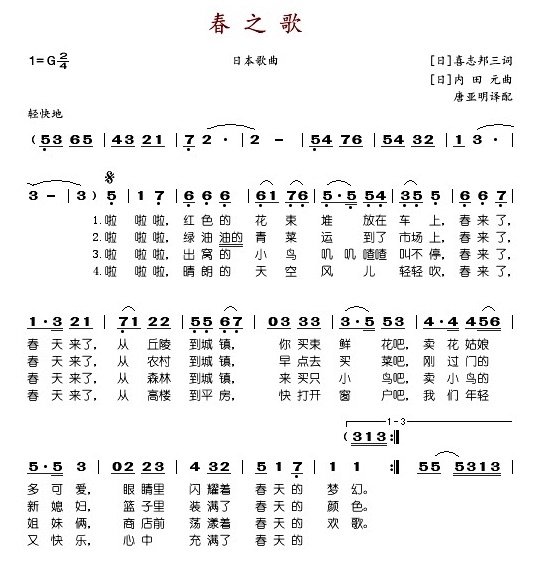
\includegraphics[height=\textheight]{dongxiao/日本-春之歌.jpg}

\section{樱花}
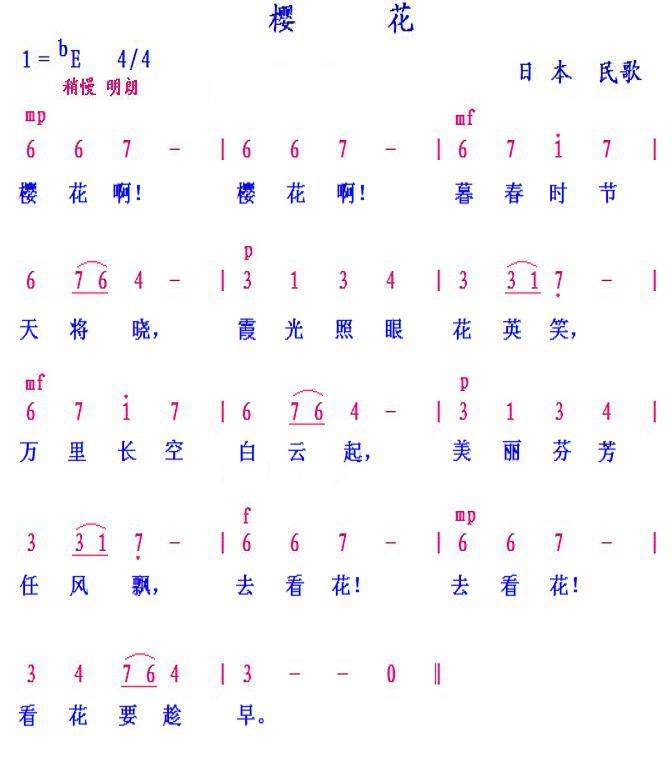
\includegraphics[width=\textwidth]{dongxiao/日本-樱花.jpg}

\section{母亲}
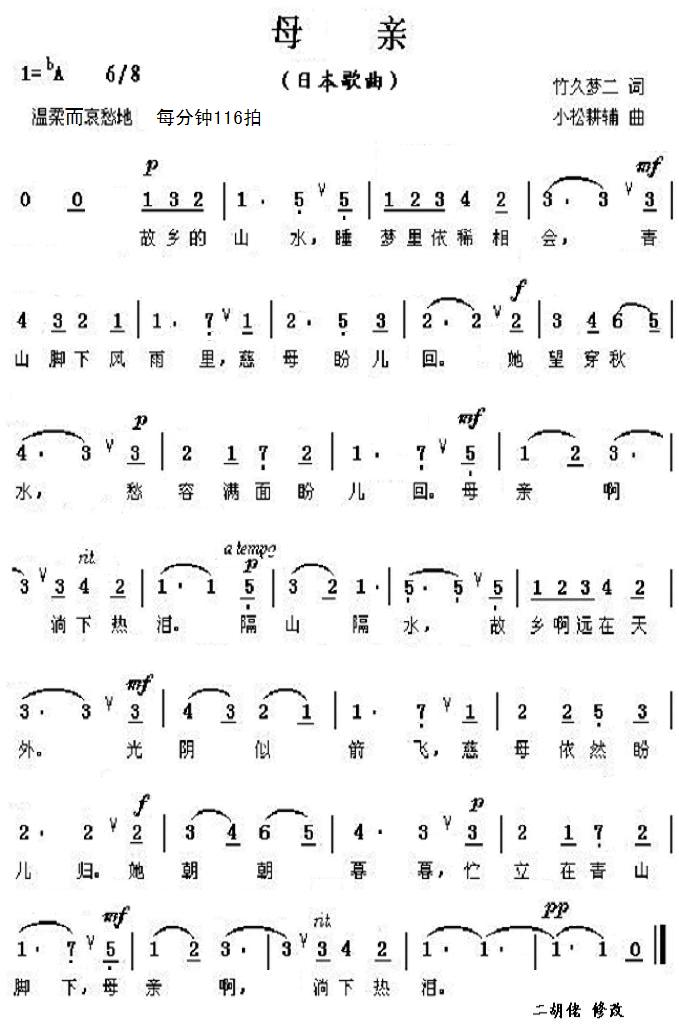
\includegraphics[height=\textheight]{dongxiao/日本-母亲.jpg}

\section{洁白的雪花}
    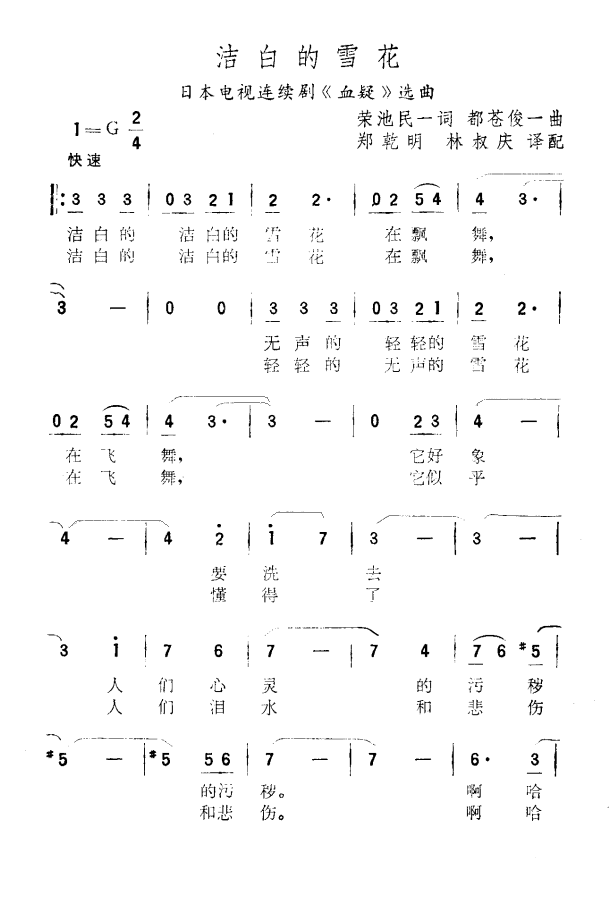
\includegraphics[height=\textheight]{dongxiao/日本-洁白的雪花.png}
\section{海边之歌}
    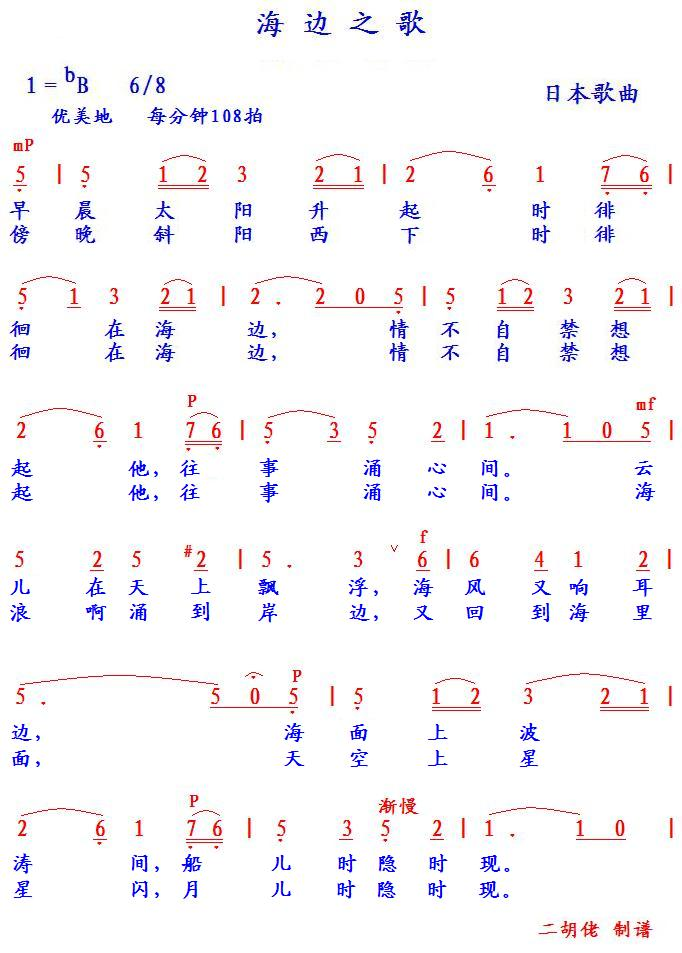
\includegraphics[height=\textheight]{dongxiao/日本-海边之歌.jpg}

\section{白云姑娘}
    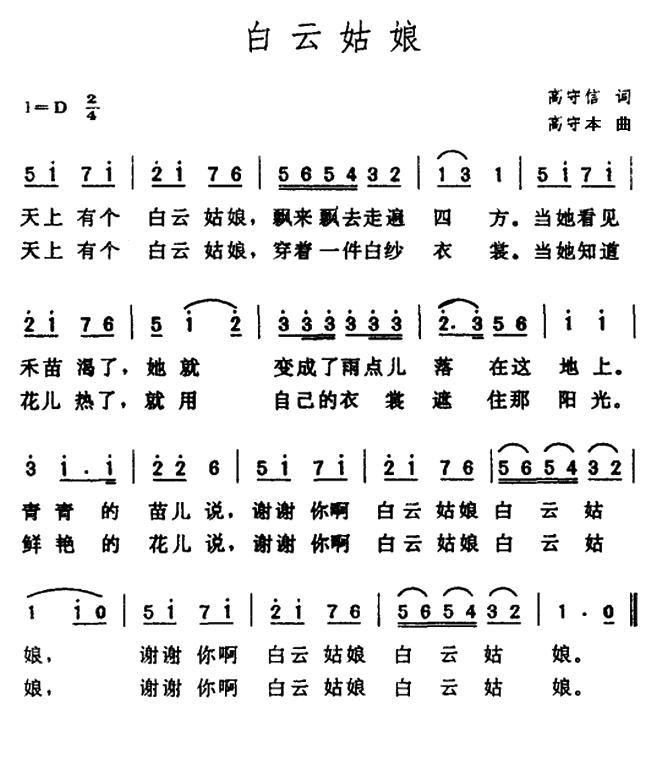
\includegraphics[width=\textwidth]{dongxiao/日本-白云姑娘.jpg}
\section{雨中岚山}
    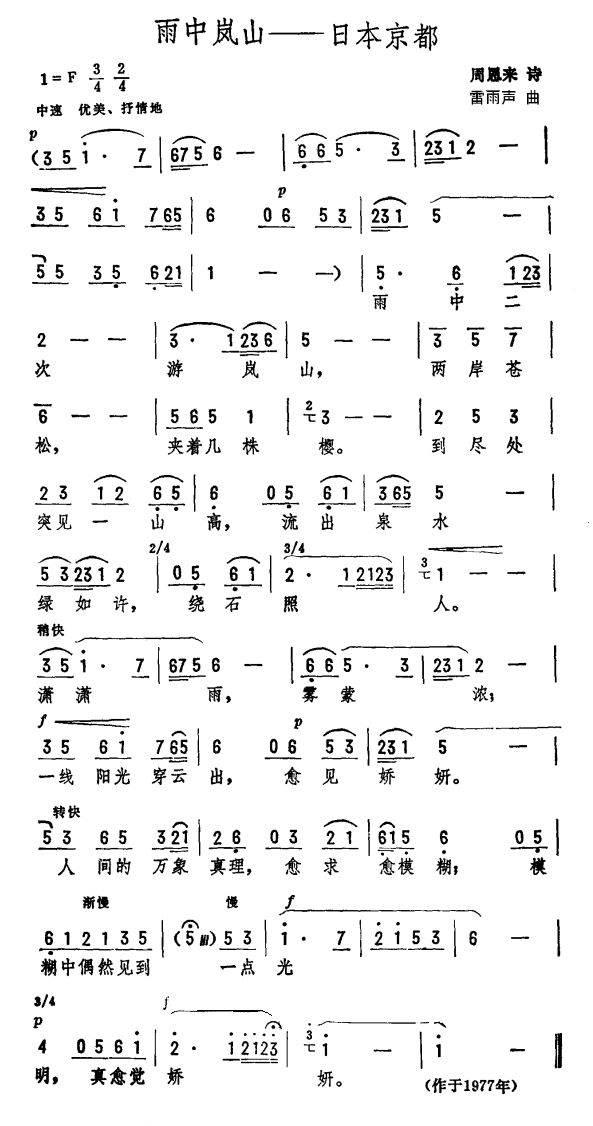
\includegraphics[height=\textheight]{dongxiao/日本-雨中岚山.png}
\section{鹰}
    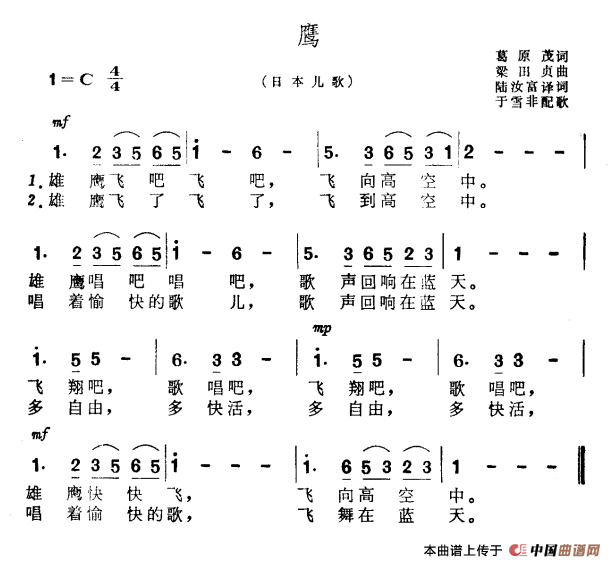
\includegraphics[width=\textwidth]{dongxiao/日本-鹰.png}
\section{洞箫悠悠}
    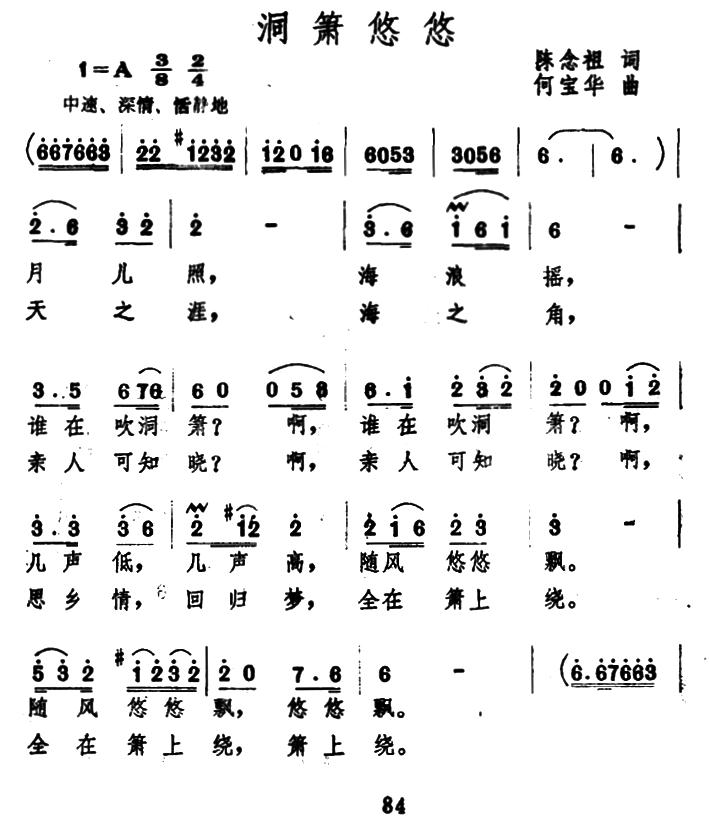
\includegraphics[width=\textwidth]{dongxiao/洞箫悠悠.jpg}

\section{秋窗风雨}
    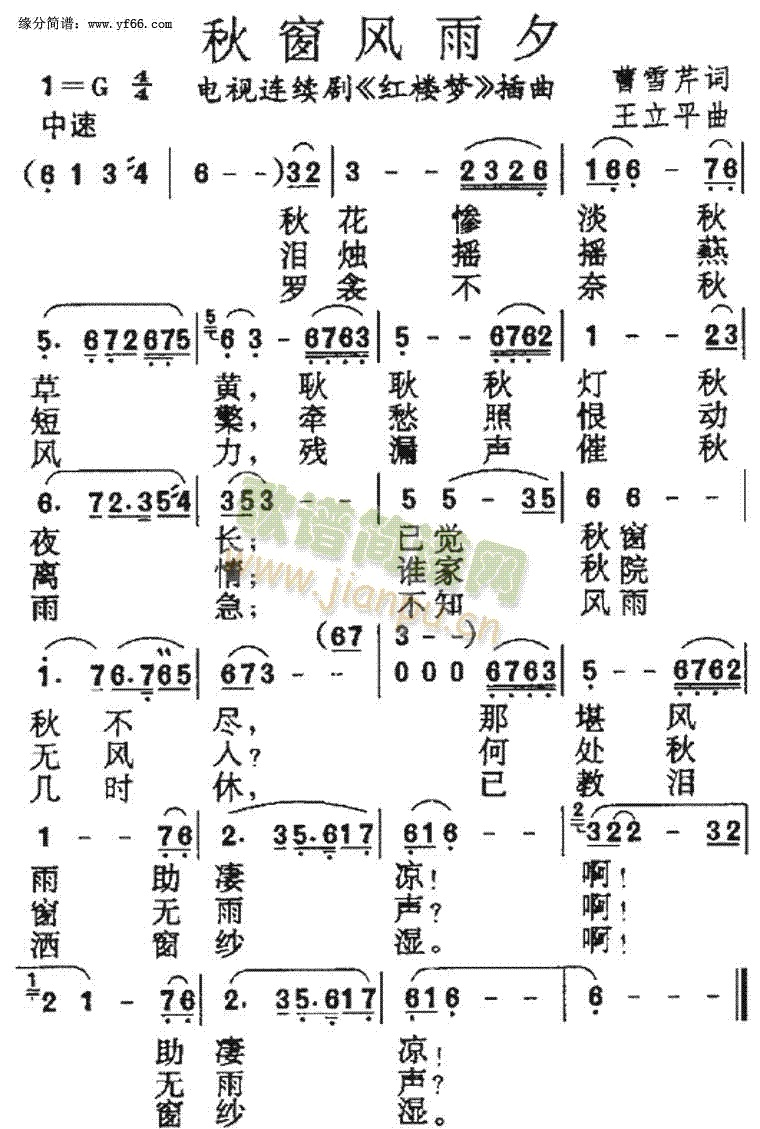
\includegraphics[width=\textwidth]{dongxiao/秋窗风雨.jpg}
\section{红楼梦引}
    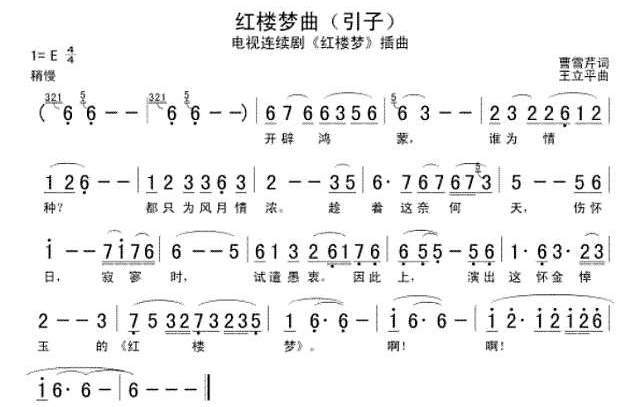
\includegraphics[width=\textwidth]{dongxiao/红楼梦引.jpg}
\section{红豆曲}
    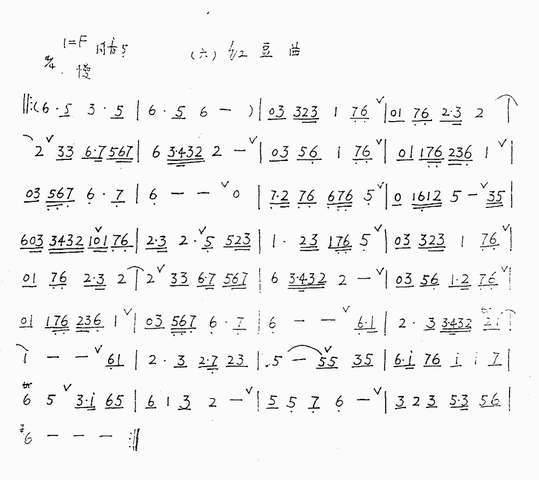
\includegraphics[width=\textwidth]{dongxiao/红豆曲.jpg}
\section{西湖春}
    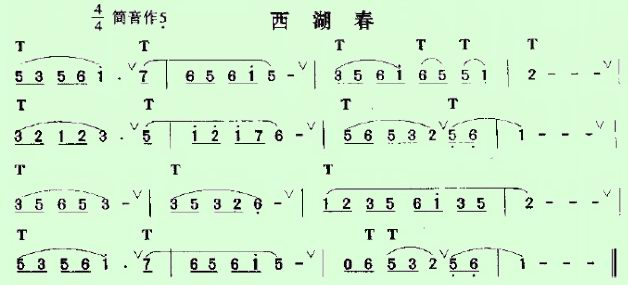
\includegraphics[width=\textwidth]{dongxiao/西湖春.jpg}
    
\section{孤星独吟}
    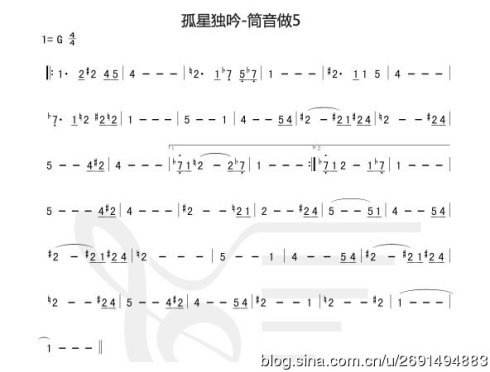
\includegraphics[width=\textwidth]{dongxiao/孤星独吟.jpg}
\section{雨醉江南}
    \includegraphics[width=\textwidth]{dongxiao/雨醉江南.jpg}
\section{枉凝眉}
    \includegraphics[width=\textwidth]{dongxiao/枉凝眉.jpg}
\section{月夜思念}
    \includegraphics[width=\textwidth]{dongxiao/月夜思念.jpg}
\section{特血丹心}
    \includegraphics[width=\textwidth]{dongxiao/铁血丹心.jpg}
    
\section{青玉按-元夕}
    \includegraphics[width=\textwidth]{dongxiao/202003231431青玉按.png}
\section{卷珠帘}
    \includegraphics[width=\textwidth]{dongxiao/202003231629卷珠帘.jpg}
\section{玉楼春}
    \includegraphics[width=\textwidth]{dongxiao/202003231632玉楼春.jpg}
\section{寒香}
    \includegraphics[width=\textwidth]{dongxiao/202003231845寒香.jpg}
    
\section{初见}
    \includegraphics[width=\textwidth]{dongxiao/2020323初见.jpg}
\section{白桦林}
    \includegraphics[width=\textwidth]{dongxiao/20200323白桦林.jpg}
\section{凤凰台上忆吹箫}
    \includegraphics[width=\textwidth]{dongxiao/202003231853凤凰台上忆吹箫.jpg}
\section{揽工调}
    \includegraphics[width=\textwidth]{dongxiao/202003231857揽工调.jpg}
    
\section{凄凉犯}
    \includegraphics[width=\textwidth]{dongxiao/202003231858凄凉犯.jpg}
\section{清官谣}
    \includegraphics[width=\textwidth]{dongxiao/202003231858清官谣.jpg}
\section{风留念}
    \includegraphics[width=\textwidth]{dongxiao/202003231859风留念.jpg}
\section{墨香-长安曲}
    \includegraphics[width=\textwidth]{dongxiao/202003231859墨香-长安曲.jpg}
\end{document}
